% ----------------------------------------------------------------------
%                   LATEX TEMPLATE FOR PhD THESIS
% ----------------------------------------------------------------------

% based on Harish Bhanderi's PhD/MPhil template, then Uni Cambridge
% http://www-h.eng.cam.ac.uk/help/tpl/textprocessing/ThesisStyle/
% corrected and extended in 2007 by Jakob Suckale, then MPI-CBG PhD programme
% and made available through OpenWetWare.org - the free biology wiki


%: Style file for Latex
% Most style definitions are in the external file PhDthesisPSnPDF.
% In this template package, it can be found in ./Latex/Classes/
%\documentclass[twoside,11pt]{Latex/Classes/PhDthesisPSnPDF}
\documentclass[twoside,12pt]{Latex/Classes/PhDthesisPSnPDF}
\usepackage{setspace}
\usepackage{placeins} 
\usepackage{xgreek}
%\doublespacing

%: Colore or not 
% Change comments accourtigly for B/W or Colored copies 
\newif\ifcolore
%\coloretrue
\colorefalse

%: Macro file for Latex
% Macros help you summarise frequently repeated Latex commands.
% Here, they are placed in an external file /Latex/Macros/MacroFile1.tex
% An macro that you may use frequently is the figuremacro (see introduction.tex)
% This file contains macros that can be called up from connected TeX files
% It helps to summarise repeated code, e.g. figure insertion (see below).

% insert a centered figure with caption and description
% parameters 1:filename, 2:title, 3:description and label
\newcommand{\figuremacro}[3]{
	\begin{figure}[htbp]
		\centering
		\includegraphics[width=1\textwidth]{#1}
		\caption[#2]{\textbf{#2} - #3}
		\label{#1}
	\end{figure}
}

% insert a centered figure with caption and description AND WIDTH
% parameters 1:filename, 2:title, 3:description and label, 4: textwidth
% textwidth 1 means as text, 0.5 means half the width of the text
\newcommand{\figuremacroW}[4]{
	\begin{figure}[htbp]
		\centering
		\includegraphics[width=#4\textwidth]{#1}
		\caption[#2]{\textbf{#2} - #3}
		\label{#1}
	\end{figure}
}

% inserts a figure with wrapped around text; only suitable for NARROW figs
% o is for outside on a double paged document; others: l, r, i(inside)
% text and figure will each be half of the document width
% note: long captions often crash with adjacent content; take care
% in general: above 2 macro produce more reliable layout
\newcommand{\figuremacroN}[3]{
	\begin{wrapfigure}{o}{0.5\textwidth}
		\centering
		\includegraphics[width=0.48\textwidth]{#1}
		\caption[#2]{{\small\textbf{#2} - #3}}
		\label{#1}
	\end{wrapfigure}
}

% predefined commands by Harish
\newcommand{\PdfPsText}[2]{
  \ifpdf
     #1
  \else
     #2
  \fi
}

\newcommand{\IncludeGraphicsH}[3]{
  \PdfPsText{\includegraphics[height=#2]{#1}}{\includegraphics[bb = #3, height=#2]{#1}}
}

\newcommand{\IncludeGraphicsW}[3]{
  \PdfPsText{\includegraphics[width=#2]{#1}}{\includegraphics[bb = #3, width=#2]{#1}}
}

\newcommand{\InsertFig}[3]{
  \begin{figure}[!htbp]
    \begin{center}
      \leavevmode
      #1
      \caption{#2}
      \label{#3}
    \end{center}
  \end{figure}
}


%%% Local Variables: 
%%% mode: latex
%%% TeX-master: "~/Documents/LaTeX/CUEDThesisPSnPDF/thesis"
%%% End: 

\usepackage{amsmath}
\usepackage{amssymb}
\usepackage{mathrsfs}
\selectlanguage{greek}
 

%: ----------------------------------------------------------------------
%:                  TITLE PAGE: name, degree,..
% ----------------------------------------------------------------------
% below is to generate the title page with crest and author name

%if output to PDF then put the following in PDF header
\ifpdf  
    \pdfinfo { /Title  (Evolutionary Algorithm-based Design-Optimization Methods in Turbomachinery)
               /Creator (Stylianos Kyriacou )
               /Producer (Stylianos Kyriacou )
               /Author (Stylianos Kyriacou stelios.kyriacou@gmail.com)
               /CreationDate (D:YYYYMMDDhhmmss)  %format D:YYYYMMDDhhmmss
               /ModDate (D:YYYYMMDDhhmm)
               /Subject (Evolutionary Algorithm-based Design-Optimization Methods in Turbomachinery)
               /Keywords (Optimization, Evolutionary Algorithms, Metamodels, Turbo-machinery) }
    \pdfcatalog { /PageMode (/UseOutlines)
                  /OpenAction (fitbh)  }
\fi


\title{Evolutionary Algorithm-based Design-Optimization Methods in Turbomachinery}



% ----------------------------------------------------------------------
% The section below defines www links/email for author and institutions
% They will appear on the title page of the PDF and can be clicked
\ifpdf
  \author{\href{mailto:stelios.kyriacou@gmail.com}{Stylianos Kyriacou}}
%  \cityofbirth{born in XYZ} % uncomment this if your university requires this
%  % If city of birth is required, also uncomment 2 sections in PhDthesisPSnPDF
%  % Just search for the "city" and you'll find them.
  \collegeordept{\href{http://www.ntua.gr}{Mechanical Engineering}}
  \university{\href{http://www.ntua.gr}{National Technical University of Athens}}

  % The crest is a graphics file of the logo of your research institution.
  % Place it in ./0_frontmatter/figures and specify the width
  \crest{\includegraphics[width=4cm]{pyrforos}}
  
% If you are not creating a PDF then use the following. The default is PDF.
\else
  \author{Stylianos Kyriacou}
%  \cityofbirth{born in XYZ}
  \collegeordept{Mechanical Engineering, Parallel CFD \& Optimization Unit.}
  \university{National Technical University of Athens.}
  \crest{\includegraphics[width=4cm]{pyrforos}}
\fi

%\renewcommand{\submittedtext}{change the default text here if needed}
\degree{Philosophi\ae Doctor (PhD)}
\degreedate{year month}


% ----------------------------------------------------------------------
       
% turn of those nasty overfull and underfull hboxes
\hbadness=10000
\hfuzz=50pt


%: --------------------------------------------------------------
%:                  FRONT MATTER: dedications, abstract,..
% --------------------------------------------------------------

\begin{document}

%\language{greek}

% sets line spacing
\renewcommand\baselinestretch{1.0}
\baselineskip=18pt plus1pt


%: ----------------------- generate cover page ------------------------

%\maketitle  % command to print the title page with above variables

%
\selectlanguage{greek}
\begin{titlepage}
\thispagestyle{empty}
%
%
%
\begin{flushleft}
\mbox{
\begin{minipage}[c]{0.2\textwidth}
%   \scalebox{.15}{\epsfig{file=pyrforos.eps}}
   \scalebox{.2}{\includegraphics{pyrforos}}
\end{minipage}
\begin{minipage}[c]{30em}
   \raggedright
   \sc \bf
   {\large Εθνικό Μετσόβιο Πολυτεχνείο} \\
   Σχολή Μηχανολόγων Μηχανικών \\
   Τομέας Ρευστών \\
   Εργαστήριο Θερμικών Στροβιλομηχανών\\
   Μονάδα Παράλληλης Υπολογιστικής Ρευστοδυναμικής \& Βελτιστοποίησης
\end{minipage}
}
\end{flushleft}

\vskip  3cm

\begin{center}
{\large \bf Μέθοδοι Σχεδιασμού-Βελτιστοποίησης στις Στροβιλομηχανές βασισμένες στους
Εξελικτικούς Αλγορίθμους}
\vskip  2cm
Διδακτορική Διατριβή
\vskip  1cm
{\bf Στυλιανός Α. Κυριάκου}
\vskip  1cm
%(Κείμενο υπό διόρθωση)

\vskip  4cm
Επιβλέπων : ΚΥΡΙΑΚΟΣ Χ. ΓΙΑΝΝΑΚΟΓΛΟΥ
\vskip .1cm
Καθηγητής ΕΜΠ

\vskip  2cm
 Αθήνα, 2013
\end{center}

\end{titlepage}


%: ----------------------- cover page back side ------------------------
% Your research institution may require reviewer names, etc.
% This cover back side is required by Dresden Med Fac; uncomment if needed.



%: ----------------------- abstract ------------------------

% Your institution may have specific regulations if you need an abstract and where it is to be placed in the document. The default here is just after title.

%
% Thesis Abstract -----------------------------------------------------


\begin{abstractslongGR}    %uncommenting this line, gives a different abstract heading
\selectlanguage{greek}
%\begin{abstracts}        %this creates the heading for the abstract page
Σκοπός της διδακτορικής διατριβής είναι να εμπλουτίσει/επεκτείνει υπάρχουσες μεθόδους (και λογισμικό) βελτιστοποίησης το οποίο βασίζεται στους εξελικτικούς αλγορίθμους (ΕΑ) ώστε, όταν χρησιμοποιείται σε πραγματικά, μεγάλης κλίμακας προβλήματα, να μειώνεται σημαντικά ο χρόνος αναμονής του σχεδιαστή, κάνοντας τη διαδικασία σχεδιασμού-βελτιστοποίησης «αποδεκτή» σε βιομηχανικό περιβάλλον. Οι προτεινόμενες μέθοδοι και το προγραμματιζόμενο λογισμικό εφαρμόζονται σε ευρύ φάσμα εφαρμογών σχεδιασμού-βελτιστοποίησης στις στροβιλομηχανές, θερμικές και υδροδυναμικές, βιομηχανικού ενδιαφέροντος.

Σε επίπεδο λογισμικού, οι προτεινόμενες μέθοδοι υλοποιούνται εντασσόμενες στο γενικής χρήσης λογισμικό βελτιστοποίησης \english{EASY (Evolutionary Algorithm System)} της ΜΠΥΡ\&Β/ΕΘΣ. Εκμεταλλεύονται τις προϋπάρχουσες δυνατότητες του λογισμικού \english{EASY}, στις οποίες συμπεριλαμβάνονται η «έξυπνη» χρήση τεχνητών νευρωνικών δικτύων (ως μεταπρότυπα, δηλαδή χαμηλού κόστους προσεγγιστικά πρότυπα αξιολόγησης, υποκατάστατα του λογισμικού υπολογιστικής ρευστοδυναμικής – αλγόριθμος \english{MAEA: Metamodel-assisted EA)}, σχήματα κατανεμημένης ανίχνευσης του χώρου των λύσεων \english{(DEA: Distributed EA)}, ιεραρχικά ή πολυεπίπεδα σχήματα βελτιστοποίησης, ο υβριδισμός με μεθόδους βελτιστοποίησης διαφορετικές των ΕΑ και, φυσικά, η χρήση πολυεπεξεργασίας. Καλύπτουν προβλήματα μονοκριτηριακής ή πολυκριτηριακής βελτιστοποίησης, με ή χωρίς περιορισμούς.

Η συνεισφορά της διατριβής, σε σχέση με την προαναφερθείσα υποδομή, εντοπίζεται κυρίως στα παρακάτω τρία σημεία:
	α) Προτείνεται και πιστοποιείται μια πρωτότυπη διαδικασία σχεδιασμού νέων προϊόντων (εδώ στροβιλομηχανών) που βασίζεται σε ένα μικρό αριθμό διαθέσιμων αρχειοθετημένων σχεδιασμών, οι οποίοι θεωρούνται βέλτιστοι ή, έστω, αποδεκτοί, για λειτουργία σε διαφορετικές συνθήκες. Η προτεινόμενη διαδικασία αποτελεί απάντηση στον ενδοιασμό των μηχανικών της βιομηχανίας για το αν κάθε νέος σχεδιασμός προϊόντος πρέπει να ξεκινά «από το μηδέν» ή μπορεί να στηριχθεί στην υπάρχουσα εμπειρία. Για την εφαρμογή της προτεινόμενης μεθόδου, πρέπει αρχικά να απομονωθεί ένα μικρό σύνολο «σχετικών» σχεδιασμών του παρελθόντος. Αν λ.χ. το τρέχον πρόβλημα αφορά το σχεδιασμό μιας στροβιλομηχανής σε συνθήκες «Α», με στόχους «Β» και περιορισμούς «Γ», το σύνολο αυτό μπορεί να αποτελείται από ένα μονοψήφιο αριθμό στροβιλομηχανών που έχουν σχεδιαστεί στο παρελθόν για λειτουργία σε συνθήκες διαφορετικές μεν, πλησίον δε των «Α», με ίδιους ή περίπου  ίδιους στόχους, με περισσότερους ή λιγότερους συναφείς περιορισμούς. Ο τρόπος επιλογής του συνόλου αυτών των «σχετικών» σχεδιασμών, οι οποίοι πλέον θα αποκαλούνται «σχεδιασμοί βάσης»,  δεν εμπίπτει στα ενδιαφέροντα της διατριβής. Επίσης, δεν εμπίπτει η διαδικασία κοινής παραμετροποίησής τους, για την περίπτωση που αυτή δεν υφίσταται, μιας και αυτό μπορεί να πραγματοποιηθεί με πολλούς τρόπους. Η διατριβή προτείνει ένα νέο μαθηματικό τρόπο έκφρασης κάθε νέου σχεδιασμού συναρτήσει των σχεδιασμών βάσης. Ο τρόπος αυτός παρακάμπτει ουσιαστικά την παραμετροποίηση της σχεδιαζόμενης γεωμετρίας, η οποία εκ των πραγμάτων μπορεί να εισάγει εκατοντάδες βαθμούς ελευθερίας, καθυστερώντας έτσι τη σύγκλιση της βασισμένης σε ΕΑ μεθόδου βελτιστοποίησης. Αντ’ αυτών, εισάγει ένα πραγματικά μικρό πλήθος νέων μεταβλητών σχεδιασμού αλλά και τον καθορισμό περιοχών  μεγαλύτερης σημαντικότητας, με όφελος τη σημαντική μείωση του χρόνου βελτιστοποίησης. Επιπλέον σημαντικό κέρδος από τη νέα παραμετροποίηση αποτελεί το ότι τα όρια των νέων μεταβλητών σχεδιασμού προκύπτουν εύκολα, ουσιαστικά «αυτόματα» και χωρίς παρέμβαση του χρήστη. Η προτεινόμενη μέθοδος προγραμματίστηκε συμπληρωματικά στον \english{EASY} και χρησιμοποιήθηκε για το σχεδιασμό θερμικών και υδροδυναμικών μηχανών με μιας τάξης μεγέθους κέρδος σε υπολογιστικό χρόνο, για την επίτευξη  παρόμοιας ποιότητας σχεδιασμών.       
               
	β)  Προτείνεται μέθοδος εντοπισμού και, κυρίως, χρήσης των όποιων συσχετίσεων μεταξύ των μεταβλητών σχεδιασμού για την περαιτέρω επιτάχυνση των κλασικών ΕΑ, επεμβαίνοντας στους τελεστές εξέλιξης  Αυτό επιτυγχάνεται μέσω της δυναμικά (δηλαδή σε κάθε γενιά) ανανεούμενης επαναδιατύπωσης του προβλήματος βελτιστοποίησης ώστε να χειρίζεται κατά το δυνατό μη-συσχετιζόμενες (διαχωρίσιμες) μεταβλητές σχεδιασμού. Ο λόγος που μια τέτοια αντιμετώπιση επιφέρει κέρδος στο χρόνο βελτιστοποίησης είναι ότι οι ΕΑ, εκ φύσεως, κερδίζουν σημαντικά σε ταχύτητα όταν χειρίζονται προβλήματα διαχωρίσιμων μεταβλητών σχεδιασμού. Υπενθυμίζεται ότι κάθε πρόβλημα ελαχιστοποίησης μιας συνάρτησης Ν διαχωρίσιμων μεταβλητών μπορεί να αντιμετωπιστεί ως Ν προβλήματα ελαχιστοποίησης μιας συνάρτησης μιας μεταβλητής, με συνολικά μικρότερο υπολογιστικό κόστος.  Αυτό εκμεταλλεύεται η προτεινόμενη μέθοδος. Προαπαίτηση για την υλοποίηση μιας τέτοιας μεθόδου είναι η αυτόματη μετατροπή του πραγματικού προβλήματος σε πρόβλημα διαχωρίσιμων μεταβλητών. Αυτό πραγματοποιείται με χρήση της μεθόδου ανάλυσης σε κύριες συνιστώσες (ΑσΚΣ, \english{Principal Component Analysis, PCA}). Σε προβλήματα πολυκριτηριακής βελτιστοποίησης, η ΑσΚΣ εφαρμόζεται στο σύνολο των επιλέκτων κάθε γενιάς και, ουσιαστικά, πραγματοποιεί κατάλληλη «στροφή» του χώρου σχεδιασμού. Η «στροφή» αυτή απαιτεί την επίλυση ενός προβλήματος ιδιοτιμών. Αποδεικνύεται ότι ο προκύπτων χώρος, ίδιας διάστασης με το χώρο σχεδιασμού, ο οποίος καθορίζεται με άξονες τα ιδιοδιανύσματα (τις λεγόμενες «κύριες συνιστώσες») που προκύπτουν από την διαδικασία ΑσΚΣ, έχει τις κατά το δυνατό μη-συσχετιζόμενες μεταβλητές σχεδιασμού. Οι τελεστές εξέλιξης (διασταύρωση, μετάλλαξη, κλπ) εφαρμόζονται στις νέες μεταβλητές σχεδιασμού, προκύπτουν οι νέοι απόγονοι, οι οποίοι τελικά επαναφέρονται (με «αντίθετη στροφή») στον αρχικό-πραγματικό χώρο σχεδιασμού. Η προτεινόμενη μέθοδος προγραμματίστηκε συμπληρωματικά στον \english{EASY} και αρχικά πιστοποιήθηκε σε μαθηματικές συναρτήσεις και ψευδο-μηχανολογικά προβλήματα της βιβλιογραφίας. Στη συνέχεια, χρησιμοποιήθηκε για το σχεδιασμό του δρομέα ενός υδροστροβίλου  \english{HYDROMATRIX\circledR} με κέρδος την αναπαραγωγή παρόμοιας ποιότητας σχεδιασμών στο μισό χρόνο (μισός αριθμός κλήσεων του λογισμικού αξιολόγησης) σε σχέση με τον κλασικό EA.  
 
	γ) Ως προς τον ΕΑ που υποβοηθείται από μεταπρότυπα (\english{MAEA}, στη λογική της προσεγγιστικής προ-αξιολόγησης – ΠΠΑ – των ατόμων κάθε γενιάς με τεχνητά νευρωνικά δίκτυα) προτείνεται και πιστοποιείται μέθοδος η οποία αντιμετωπίζει με επιτυχία ένα σημαντικό πρόβλημα τέτοιων μεθόδων όταν χρησιμοποιούνται σε προβλήματα μεγάλης διάστασης. Είναι γνωστό από τη μέχρι τώρα εμπειρία από τη χρήση \english{MAEA} ότι το κέρδος (συγκριτικά με τους κλασικούς ΕΑ) μειώνεται όταν η διάσταση του χώρου σχεδιασμού αυξάνει σημαντικά. Αυτή η συμπεριφορά οφείλεται (α) στο ότι η έναρξη χρήσης των τεχνητών νευρωνικών δικτύων καθυστερεί, αναμένοντας την καταγραφή επαρκών ήδη αξιολογημένων υποψηφίων λύσεων στη βάση δεδομένων από την οποία αντλούνται τα δείγματα εκπαίδευσης των μεταπροτύπων και (β) στο ότι η αξιοπιστία των νευρωνικών δικτύων φθίνει αυξάνοντας τον αριθμό εισόδων σε αυτά (πλήθος μεταβλητών σχεδιασμού). Η προτεινόμενη αντιμετώπιση αυτού του προβλήματος βασίζεται στην ελεγχόμενη μείωση των εισόδων (κρατώντας, ουσιαστικά, τις περισσότερο αντιπροσωπευτικές) του νευρωνικού δικτύου (εδώ, δικτύου ακτινικής βάσης, \english{radial basis function network, RBF}) που χρησιμοποιείται  ως μεταπρότυπο.  Χρησιμοποιώντας και πάλι ανάλυση σε κύριες συνιστώσες, στο ίδιο σύνολο δυναμικά ανανεούμενων επιλέκτων, πραγματοποιείται εκ νέου στροφή/ευθυγράμμιση του χώρου σχεδιασμού με τις κύριες συνιστώσες λαμβάνοντας υπόψη την σημαντικότητα της κάθε μεταβλητής. Η τελευταία είναι αντιστρόφως ανάλογη της τιμής της σχετικής ιδιοτιμής που προέκυψε από την ΑσΚΣ  που έγινε κατά τη διάρκεια της μεθόδου. Το επιπλέον στοιχείο, εδώ, είναι ότι στο «στραμμένο» πλέον χώρο σχεδιασμού, γίνεται αποκοπή και συγκρατείται μικρός αριθμός των πλέον σημαντικών «στραμμένων» μεταβλητών σχεδιασμού. Με τις τελευταίες, και μόνο αυτές, εκπαιδεύεται το δίκτυο \english{RBF}. Η τεχνική αυτή οδηγεί σε περαιτέρω μείωση του χρόνου βελτιστοποίησης αφού τα μεταπρότυπα παρέχουν προβλέψεις υψηλότερης αξιοπιστίας αλλά και μπορούν να  ξεκινήσουν να χρησιμοποιούνται νωρίτερα κατά τη διαδικασία βελτιστοποίησης. Η μέθοδος χρησιμοποιήθηκε, με ή χωρίς την επικουρική χρήση της μεθόδου (α) και σε συνδυασμό με τη μέθοδο (β) στο σχεδιασμό-βελτιστοποίηση 2Δ και 3Δ πτερύγωσης συμπιεστή με κέρδος τη μείωση του χρόνου βελτιστοποίησης στο 1/3 του χρόνου ενός κλασικού \english{MAEA}.        

Οι τεχνικές που αναπτύχθηκαν στην παρούσα διδακτορική εργασία χρησιμοποιήθηκαν στο σχεδιασμό και βελτιστοποίηση ενός καινοτόμου τύπου υδροστροβίλου “\english{HYDROMATRIX\circledR}” ιδανικού για τοποθεσίες μικρού ύψους (\english{H=5-10m, Q$>$60m3/s}). Οι υδροστρόβιλοι “\english{HYDROMATRIX\circledR}”, πατενταρισμένοι από την εταιρία \english{Andritz-Hydro} συνδυάζουν τη υψηλή αποδοτικότητα (10\% υψηλότερη από άλλους τύπους υδροστροβίλων χαμηλού ύψους) με το χαμηλό κόστος εγκατάστασης, με περιβαλλοντικά και οικονομικά οφέλη. Κάνοντας χρήση των τεχνικών που αναπτύχθηκαν στην παρούσα διδακτορική διατριβή, επιτεύχθηκε μείωση του συνολικού χρόνου σχεδιασμού (όχι μόνο της διαδικασίας βελτιστοποίησης) σε ποσοστό μεγαλύτερο του 50\% από 120-140 μέρες σε μόλις 50.  Η προαναφερθείσα μείωση του συνολικού χρόνου σχεδιασμού και η συνεπαγόμενη μείωση του κόστους σχεδιασμού μετατρέπουν σε οικονομικά επικερδή τη χρήση “\english{HYDROMATRIX\circledR}” σε ακόμη μικρότερα ύψη, \english{H=2-5m}, και παροχές μικρότερες των \english{60m3/s}. Αξίζει να σημειωθεί ότι η διαθεσιμότητα τοποθεσιών με αυτά τα χαρακτηριστικά, μόνο στην Ευρώπη, είναι της τάξης των \english{6000 GWh/year} με ότι αυτό συνεπάγεται τόσο σε οικονομικά οφέλη όσο και σε περιβαλλοντολογικά λόγω της αντίστοιχης μείωσης των εκπομπών \english{CO2}. 

Στο πλαίσιο συνεργασιών με την εταιρία \english{Andritz-Hydro}, η οποία χρηματοδότησε τμήμα της  παρούσας διατριβής, οι αναπτυχθείσες τεχνικές εφαρμόστηκαν και σε μια σειρά άλλων σχεδιασμών υδροδυναμικών μηχανών ή συνιστωσών τους. Περισσότερο αναλυτικά, με βάση τις τεχνικές αυτές οργανώθηκαν διαδικασίες σχεδιασμού δρομέων όλων των κλασικών τύπων υδροδυναμικών στροβιλομηχανών αντίδρασης τόσο αξονικής όσο και μικτής ροής (\english{Francis, Kaplan, Bulb, Pump} και \english{Pump-Turbines}), με στόχο τόσο την αύξηση της απόδοσής τους όσο και τη βέλτιστη συνεργασία τους με τα υπόλοιπά μέρη της εγκατάστασης. Επίσης σχεδιάστηκαν σταθερές συνιστώσες υδροδυναμικών μηχανών όπως αγωγοί απαγωγής (\english{draft tubes}), με στόχο τη μέγιστη ανάκτηση πίεσης με τις ελάχιστες απώλειες και τμήματα αγωγών εισόδου υδροστροβίλων δράσης διανομείς-\english{distributors}), με στόχο την ελαχιστοποίηση του κόστους κατασκευής και απωλειών με παράλληλη αύξηση της ποιότητας της δέσμης ρευστού μετά το ακροφύσιο. Επιλεγμένο τμήμα των παραπάνω σχεδιασμών παρουσιάζεται στο κείμενο της διδακτορικής διατριβής. 

Το έργο με τίτλο «\english{HYDROACTION – Development and laboratory testing of improved action and Matrix hydro turbines designed by advanced analysis and optimization tools» (Project Number 211983)}, το οποίο χρηματοδότησε η Ευρωπαϊκή Ένωση, υποστήριξε το υπόλοιπο τμήμα της διατριβής. Το ΕΜΠ και η \english{Andritz-Hydro} υπήρξαν εταίροι στο έργο αυτό. Οι βιομηχανικής κλίμακας υπολογισμοί, στις προαναφερθείσες εφαρμογές θερμικών και υδροδυναμικών στροβιλομηχανών, πραγματοποιήθηκαν, εκ των πραγμάτων, σε πολυεπεξεργαστικά συστήματα. Ως τέτοια χρησιμοποιήθηκαν τα πολυεπεξεργαστικά συστήματα της ΜΠΥΡ\&Β/ΕΘΣ (Αθήνα) και της \english{Andritz-Hydro (Linz, Graz \& Vevey)}, ενίοτε και συνεργατικά μέσω τεχνικών \english{Grid Computing}, τις οποίες υποστηρίζει το λογισμικό \english{EASY}. 
%\end{abstracts}

\end{abstractslongGR}

% ---------------------------------------------------------------------- 


% The original template provides and abstractseparate environment, if your institution requires them to be separate. I think it's easier to print the abstract from the complete thesis by restricting printing to the relevant page.
% \begin{abstractseparate}
%   \cleardoublepage %put on right page
% Thesis Abstract -----------------------------------------------------
\begin{abstractslong}    %uncommenting this line, gives a different abstract heading
%\begin{abstracts}        %this creates the heading for the abstract page

The scope of this PhD is to propose a set of improvements to existing shape design-optimization methods in fluid dynamics based on Evolutionary Algorithms (EAs) and demonstrate their efficiency in real-world applications. Though the proposed method and the developed EA based software are both generic, this thesis focuses on applications in the fields of hydraulic and thermal turbomachines. With the proposed algorithmic variants, the optimization turn-around time is noticeably reduced with respect to that of the conventional (reference, background) methods. Though the conventional methods are computationally expensive, with the proposed add-ons, they become affordable even for large-scale industrial applications. The background design-optimization methods are based on EAs enhanced by the use of artificial neural networks, acting as surrogate evaluation models or metamodels. The design process is coupled with the necessary Computational Fluid Dynamic (CFD) software. Parallelization, in the form of concurrent evaluations of the candidate solutions within each generation of the EA, is absolutely necessary, given the high CPU cost per CFD-based evaluation. All computations were performed on the multi-processor platform of the Parallel CFD \& Optimization Unit (PCOpt) of the National Technical University of Athens (NTUA). Using the proposed optimization methods several turbomachinery design optimization problems are solved; these include the design-optimization of traditional hydraulic turbines (such as Francis turbine) and a new/innovative variation of bulb turbines, the so-called ``Hydromatrix$\circledR$", suitable for low head hydropower sites. These computations were performed in close collaboration with a major hydraulic turbine manufacturer (Andritz Hydro).  Furthermore, the compressor cascade installed at the Lab of Thermal Turbomachines of NTUA (LTT/NTUA) is optimized. This thesis presents also the application of the proposed methods and tools on a number of mathematical optimization problems, since these allow a great number of test runs to be performed at negligible CPU cost.

The most important contributions of this thesis are listed below:
	
a)	 A new design method, which fully exploits archived designs with good performance in ``similar" conditions, is proposed. In this method, EAs (either in their conventional form or in enhanced variants assisted by metamodels) solve a reformulated optimization problem, instead of the high dimensional real problem . The new unknowns are used to non-linearly weight the archived designs so as to create candidate solutions to the problem in hand; it is a great advantage of the proposed method that, by doing so, the EA avoids handling the, otherwise, great number of variables parameterizing the complex shape to be designed. Gains from the reduction of the design variables are evident. An extra gain in CPU cost arises from the statistical analysis of the archived designs that helps identifying the most important design space regions, where greater probabilities of accommodating new offspring are given. The proposed method has the additional advantage of allowing the automatic definition of the new variables upper and lower bounds.
	            
b)	 The use of principal component analysis (PCA) as a means to reveal the topological characteristics of the current generation elite set is proposed. The principal directions on the design space, as computed via PCA in each generation, are used for the rotation of the design variable coordinate system before the application of the evolution operators. This rotation suffices to transform an ill-posed optimization problem into a better-posed one. Through the proposed PCA-driven evolution operators, offspring generations of higher quality are created and, this certainly reduces the number of generations required to get the optimal solution(s). Note that this is done without truncating the design variables, as a few other method are doing.           

c)	 The same PCA technique, along with the information about the design variable importance is used to enchance the inexact pre-evaluation (IPE) phase in metamodel-assisted EAs (MAEAs). This is, herein, applied in MAEAs incorporating radial basis function (RBF) networks as metamodels, in either single- or multi-objective optimization problems. The proposed method aims at obtaining more relevant predictions of the objective function values by the online trained metamodels. To this end, the PCA-driven rotation of the design variables followed by an appropriate truncation of the less-significant among them allow the use of metamodels trained on patterns of smaller dimension. Consequently, the training can rely on a smaller number of patterns and predictions made by the RBF network are much better. The EA based search is, thus, better driven and this leads to lower CPU costs.

The gain from the use of the proposed methods, either separately or in combination, is quantified in a few mathematical test cases and, then, in real-world applications. These were solved both by the proposed method and the background optimization method. In more detail, the gain from the use of KBD is demonstrated by solving the design problem of a 3D Francis hydraulic-turbine  and that of a 2D compressor cascade. The use of an EA with PCA driven evolution operators is shown in the design-optimization of a ``Hydromatrix$\circledR$". The use of PCA to enhance the performance of metamodels in MAEAs is demonstrated in the design of a 2D compressor cascade and the optimization of the blade shape of a peripheral compressor cascade installed and measured at LTT/NTUA. 

%\end{abstracts}
\end{abstractslong}

% ---------------------------------------------------------------------- 

% \end{abstractseparate}


%: ----------------------- tie in front matter ------------------------

%\frontmatter
%Nomenclature
\thispagestyle{empty}
%
%
%
\selectlanguage{english}
{\bf Nomeclature}
\begin{table}[h!]
\begin{tabular}{ ll }
\textbf{EA} &  \greek{Εξελικτικός Αλγόριθμος}\\
\textbf{EA} & Evolutionary Algorithm \\
\\
\textbf{\greek{ΠΠΑ}} & \greek{Προσεγγιστική Προ-Αξιολόγηση}\\
\textbf{IPE} & Inexact Pre-Evaluation \\
\\
\textbf{\greek{ΥΡΔ}} & \greek{Υπολογιστική Ρευστοδυναμική}\\
\textbf{CFD} & Computational Fluid Dynamics\\
\\
\textbf{\greek{ΑσΚΣ}} & \greek{Ανάλυση σε Κύριες Συνιστώσες}\\
\textbf{PCA} & Principal Component Analysis\\
\\
\textbf{\greek{ΜΦ}} & \greek{Μερικό Φορτίο}\\
\textbf{PL}       & Part Load\\
\\
\textbf{\greek{ΠΦ}} & \greek{Πλήρες Φορτίο}\\
\textbf{FL}       & Full Load\\
\\
\textbf{\greek{ΜΑ}} & \greek{Μέγιστη Απόδοση}\\
\textbf{BE}       & Best Efficiency\\
\\
\textbf{HEA} & Hierarchical Evolutionary Algorithm \\
\\
\textbf{KBD} & Knowledge Based Design\\
\\
\textbf{MAEA} & Metamodel-Assisted Evolutionary Algorithm \\
\\
\textbf{MAEA(PCA)} & MAEA with PCA-Driven Evolution Operators\\
\\
\textbf{M(PCA)AEA(PCA)} & MAEA(PCA) with PCA-Driven Metamodels\\
\\
\textbf{TE}       & Trailing Edge\\
\\
\textbf{LE}       & Leading Edge\\
\end{tabular}
\end{table}
\selectlanguage{greek}
%% Thesis Acknowledgements ------------------------------------------------


%\begin{acknowledgementslong} %uncommenting this line, gives a different acknowledgements heading
\begin{acknowledgements}      %this creates the heading for the acknowlegments
%This thesis was performed in close collaboration with ANDRITZ HYDRO GmbH based on their experience and tools.
I would like to express my deep and sincere gratitude to my supervisor, Professor Kyriakos Giannakoglou, Lab of Thermal Turbomachines and Head of the Parallel CFD \& Optimization Unit, School of Mechanical Engineering, National Technical University of Athens. His wide knowledge and structured way of thinking have been of great value for me. His understanding, encouraging and personal guidance have provided a good basis for the present thesis.

I also would like to thank Professor K. Mathioudakis and Associate Professor J. Anagnostopoulos for their valuable comments and participation in the advisory committee of my PhD thesis.

I am deeply grateful to Erwin Oberbichler, Simon Weissenberger and Peter Grafenberger (Andritz Hydro Linz) for guiding me into the inner workings of hydraulic turbines and, above all, sharing their experience and knowledge on what the optimal turbine should really look like. I also wish to thank all of my colleges in Andritz Hydro Linz for their detailed and constructive comments, and for their important support throughout this work. 

I wish to express my warm and sincere thanks to Arno Gehrer (Andritz Hydro Graz) for sharing his ideas and concepts on optimization regarding hydraulic pumps and pump-turbines and Irida Skouteropoulou (Andritz Hydro Graz) and Kostas Tsiakas (ex Andritz Hydro Graz and, currently PhD student at NTUA) for implementing and testing them in collaboration with the optimization methods developed in this PhD thesis. Furthermore I would like to thank Etienne Parkinson and  Florent Champet (Andritz Hydro Vevey) for their ideas concerning optimization of pelton distributors. 

My warm thanks are due to Paul Pieringer and Livia Koch for providing the parameterization, grid generation and flow solver tools used for the industrial-scale hydraulic turbine optimization problems solved in this thesis.      

I warmly thank Dr. Ioannis Kampolis for laying the stable foundations on which this thesis was built upon and guiding me during my early research years. Also, I would like to thank Dr. Varvara Asouti for her valuable help in the field of Evolutionary Algorithms.

During this PhD thesis, I have collaborated with many colleagues, from the PCOpt/NTUA, for whom I have great regard. Without exception, all new ideas/methods presented in this thesis have their roots in constructive conversations with them and for that I warmly thank them.   

Also, I would like to thank Peter Kunz, Christian Fuereder, Gabriele Humer and Markus Oswald for the construction and experimental validation of the Hydromatrix$\circledR$ turbine presented in Appendix 2.

Last but not least, I owe my loving thanks to my family, Antonis, Anna and Nektaria Kyriacou.  Without their encouragement and understanding, it would have been impossible for me to finish this PhD thesis. 

The financial support of Andritz Hydro and the EU project named ``HYDROACTION-Development and laboratory testing of improved action and Matrix hydro turbines designed by advanced analysis and optimization tools" (PROJECT NUMBER : 211983) is gratefully acknowledged.

\end{acknowledgements}
%\end{acknowledgmentslong}

% ------------------------------------------------------------------------





%: ----------------------- contents ------------------------

\setcounter{secnumdepth}{3} % organisational level that receives a numbers
\setcounter{tocdepth}{3}    % print table of contents for level 3
\tableofcontents            % print the table of contents
% levels are: 0 - chapter, 1 - section, 2 - subsection, 3 - subsection


%: ----------------------- list of figures/tables ------------------------

%\listoffigures	% print list of figures

%\listoftables  % print list of tables


%: ----------------------- glossary ------------------------

% Tie in external source file for definitions: /0_frontmatter/glossary.tex
% Glossary entries can also be defined in the main text. See glossary.tex
%% this file is called up by thesis.tex
% content in this file will be fed into the main document

% Glossary entries are defined with the command \nomenclature{1}{2}
% 1 = Entry name, e.g. abbreviation; 2 = Explanation
% You can place all explanations in this separate file or declare them in the middle of the text. Either way they will be collected in the glossary.

% required to print nomenclature name to page header
\markboth{\MakeUppercase{\nomname}}{\MakeUppercase{\nomname}}


% ----------------------- contents from here ------------------------

% chemicals
\nomenclature{DAPI}{4',6-diamidino-2-phenylindole; a fluorescent stain that binds strongly to DNA and serves to marks the nucleus in fluorescence microscopy} 
\nomenclature{DEPC}{diethyl-pyro-carbonate; used to remove RNA-degrading enzymes (RNAases) from water and laboratory utensils}
\nomenclature{DMSO}{dimethyl sulfoxide; organic solvent, readily passes through skin, cryoprotectant in cell culture}
\nomenclature{EDTA}{Ethylene-diamine-tetraacetic acid; a chelating (two-pronged) molecule used to sequester most divalent (or trivalent) metal ions, such as calcium (Ca$^{2+}$) and magnesium (Mg$^{2+}$), copper (Cu$^{2+}$), or iron (Fe$^{2+}$ / Fe$^{3+}$)}



 

\begin{multicols}{2} % \begin{multicols}{#columns}[header text][space]
\begin{footnotesize} % scriptsize(7) < footnotesize(8) < small (9) < normal (10)

\printnomenclature[1.5cm] % [] = distance between entry and description
\label{nom} % target name for links to glossary

\end{footnotesize}
\end{multicols}



%: --------------------------------------------------------------
%:                  MAIN DOCUMENT SECTION
% --------------------------------------------------------------

% the main text starts here with the introduction, 1st chapter,...
\mainmatter

\renewcommand{\chaptername}{} % uncomment to print only "1" not "Chapter 1"


%: ----------------------- subdocuments ------------------------

% Parts of the thesis are included below. Rename the files as required.
% But take care that the paths match. You can also change the order of appearance by moving the include commands.


% this file is called up by thesis.tex
% content in this file will be fed into the main document

%: ----------------------- introduction file header -----------------------
\selectlanguage{greek}
\chapter{Εισαγωγή}
\ifpdf
    \graphicspath{{1_introduction/figures/PNG/}{1_introduction/figures/PDF/}{1_introduction/figures/}}
\else
    \graphicspath{{1_introduction/figures/EPS/}{1_introduction/figures/}}
\fi
Σκοπός της διδακτορικής διατριβής είναι να εμπλουτίσει και να επεκτείνει υπάρχουσες μεθόδους (και λογισμικό) βελτιστοποίησης το οποίο βασίζεται στους εξελικτικούς αλγορίθμους (ΕΑ). Στόχος του νέου λογισμικού είναι, όταν αυτό χρησιμοποιείται σε πραγματικά μεγάλης κλίμακας προβλήματα της βιομηχανίας, να μειώνεται σημαντικά ο χρόνος ολοκλήρωσης του έργου, κάνοντας τη διαδικασία σχεδιασμού-βελτιστοποίησης ελκυστική για χρήση σε βιομηχανικό περιβάλλον. Οι προτεινόμενες μέθοδοι και το προγραμματισθέν λογισμικό εφαρμόζονται σε ένα φάσμα εφαρμογών σχεδιασμού-βελτιστοποίησης στις στροβιλομηχανές, θερμικές και υδροδυναμικές, οι περισσότερες από τις οποίες είναι βιομηχανικού ενδιαφέροντος.

Σε επίπεδο λογισμικού, οι προτεινόμενες μέθοδοι υλοποιούνται εντασσόμενες στο γενικής χρήσης λογισμικό βελτιστοποίησης \english{EASY (Evolutionary Algorithm SYstem)}, της Μονάδας Παράλληλης Υπολογιστικής Ρευστοδυναμικής \& Βελτιστοποίησης του Εργαστηρίου Θερμικών Στροβιλομηχανών του ΕΜΠ (ΜΠΥΡ\&Β/ΕΘΣ), \cite{phd_Giotis,phd_Karakasis,phd_Kampolis,EASYsite}. Εκμεταλλεύονται προϋπάρχουσες δυνατότητες του λογισμικού \english{EASY}, στις οποίες συμπεριλαμβάνονται η «έξυπνη» χρήση τεχνητών νευρωνικών δικτύων (ως μεταπρoτύπων, δηλαδή προσεγγιστικών προτύπων αξιολόγησης χαμηλού κόστους, υποκατάστατων του ακριβούς αλλά και ακριβού λογισμικού υπολογιστικής ρευστοδυναμικής, ΥΡΔ – αλγόριθμος \english{MAEA: Metamodel-Assisted EA)}, σχήματα κατανεμημένης ανίχνευσης του χώρου των λύσεων μέσω ΕΑ \english{(DEA: Distributed EA)}, ιεραρχικά ή πολυεπίπεδα σχήματα βελτιστοποίησης, υβριδισμός με μεθόδους βελτιστοποίησης διαφορετικές των ΕΑ αλλά και η χρήση πολυεπεξεργασίας. Καλύπτουν δε προβλήματα μονοκριτηριακής ή πολυκριτηριακής βελτιστοποίησης, με ή χωρίς περιορισμούς.

\section{Συνεισφορά της διατριβής}
Σε σχέση με την προαναφερθείσα υποδομή, η συνεισφορά της διατριβής εντοπίζεται κυρίως στα παρακάτω τρία σημεία:

	α) Προτείνεται και πιστοποιείται μια πρωτότυπη διαδικασία σχεδιασμού στροβιλομηχανών ή συνιστωσών αυτών, η οποία βασίζεται σε ένα μικρό αριθμό διαθέσιμων αρχειοθετημένων παρόμοιων σχεδιασμών υψηλής ποιότητας. Οι τελευταίοι θεωρείται ότι αποτελούν δοκιμασμένες υπάρχουσες λύσεις σε συναφή προβλήματα τα οποία, συνήθως, αφορούν λειτουργία σε λίγο διαφορετικές συνθήκες. Πάντως, ουδόλως υπονοείται ότι οι χρησιμοποιούμενοι αρχειοθετημένοι σχεδιασμοί, για τις δικές τους συνθήκες λειτουργίας, είναι βέλτιστοι (με την αυστηρή έννοια του όρου). Η προτεινόμενη διαδικασία θα αναφέρεται ως \english{Knowledge Based Design} ή \english{KBD}. Η διαδικασία \english{KBD} επιχειρεί να δώσει απάντηση στον ενδοιασμό των μηχανικών της βιομηχανίας για το αν κάθε νέος σχεδιασμός πρέπει να ξεκινά «από το μηδέν» ή μπορεί να στη-ριχθεί στην υπάρχουσα εμπειρία. Για την εφαρμογή της μεθόδου \english{KBD}, πρέπει αρ-χικά να απομονωθεί ένα μικρό σύνολο «συναφών» σχεδιασμών του παρελθόντος. Αν λ.χ. το τρέχον πρόβλημα αφορά στο σχεδιασμό μιας στροβιλομηχανής σε συνθήκες «Α», με στόχους «Β» και περιορισμούς «Γ», το σύνολο αυτό μπορεί να αποτελείται από ένα (συνήθως μονοψήφιο) αριθμό στροβιλομηχανών που έχουν σχεδιαστεί στο παρελθόν και ήδη λειτουργούν με καλή απόδοση σε συνθήκες διαφορετικές μεν, πλησίον δε των «Α», για ίδια ή περίπου ίδια με τα «Β» κριτήρια απόδοσης («στόχους» στην ορολογία των μεθόδων βελτιστοποίησης) και ικανοποιούν περιορισμούς περισσότερο ή λιγότερο συναφείς με τους «Γ». Ο τρόπος επιλογής του συνόλου των απαραίτητων «συναφών» σχεδιασμών, οι οποίοι πλέον θα αποκαλούνται «σχεδιασμοί βάσης»,  δεν εμπίπτει στα ενδιαφέροντα της διατριβής. Επίσης, σε αυτά δεν εμπίπτει η διαδικασία ενιαίας παραμετροποίησης των σχεδιασμών βάσης σε τρόπο συμβατό με το προς υλοποίηση πρόβλημα σχεδιασμού. Για την περίπτωση που αυτή δεν υφίσταται, επισημαίνεται ότι αυτή μπορεί να υλοποιηθεί με πολλούς τρόπους. Η διατριβή προτείνει ένα νέο μαθηματικό τρόπο διατύπωσης του προβλήματος του  νέου σχεδιασμού συναρτήσει των σχεδιασμών βάσης. Ο τρόπος αυτός παρακάμπτει ουσιαστικά την παραμετροποίηση της σχεδιαζόμενης γεωμετρίας, η οποία εκ των πραγμάτων μπορεί να εισάγει εκατοντάδες βαθμούς ελευθερίας, με αποτέλεσμα να καθυστερεί η σύγκλιση της βασισμένης στους ΕΑ μεθόδου βελτιστοποίησης. Αντ’ αυτών, εισάγεται ένα μικρό πλήθος νέων μεταβλητών σχεδιασμού (θα ονομάζονται μεταβλητές βελτιστοποίησης ώστε να υπάρχει διάκριση με τις προηγούμενες) και καθορίζονται περιοχές  μεγαλύτερης σημαντικότητας, με όφελος την αισθητή μείωση του χρόνου βελτιστοποίησης. Επιπλέον σημαντικό κέρδος από τη νέα παραμε-τροποίηση αποτελεί το ότι τα όρια των νέων μεταβλητών σχεδιασμού προκύπτουν εύκολα, ουσιαστικά «αυτόματα» και χωρίς παρέμβαση του χρήστη. Η προτεινόμενη μέθοδος, αφού προγραμματίστηκε και εντάχθηκε στο λογισμικό \english{EASY}, χρησιμοποιήθηκε για το σχεδιασμό στροβιλομηχανών επιφέροντας κέρδος μιας τάξης μεγέθους σε υπολογιστικό χρόνο για την επίτευξη  παρόμοιας ποιότητας σχεδιασμών.       
               
	β)  Προτείνεται μέθοδος επίλυσης προβλημάτων βελτιστοποίησης που χαρακτηρίζονται απο μη-διαχωρίσιμες (ως προς τις μεταβλητές σχεδιασμού) συναρτήσεις κόστους ή καταλληλότητας, με μεγάλο αριθμό μεταβλητών σχεδιασμού. Αυτά θα ονομάζονται «κακώς-τοποθετημένα» προβλήματα βελτιστοποίησης και η αντιμετώπιση τους μέσω ΕΑ οδηγεί, σχεδόν πάντα, σε πολύ χρονοβόρους υπολογισμούς. Η προτεινόμενη μέθοδος υλοποιείται επεμβαίνοντας κατάλληλα στον τρόπο που εφαρμόζονται οι τελεστές εξέλιξης.  Αυτό επιτυγχάνεται μέσω της δυναμικά (δηλαδή, σε κάθε γενιά) ανανεούμενης επαναδιατύπωσης του προβλήματος βελτιστοποίησης, ώστε ο ΕΑ να χειρίζεται, κατά το δυνατό, προβλήματα των οποίων η συνάρτηση-στόχος να είναι διαχωρίσιμη ως προς τις μεταβλητές σχεδιασμού. Ο λόγος που μια τέτοια αντιμετώπιση επιφέρει μείωση στο χρόνο επίλυσης ενός προβλήματος βελτιστοποίησης είναι ότι οι ΕΑ, εκ φύσεως, κερδίζουν σημαντικά σε ταχύτητα όταν χειρίζονται προβλήματα ελαχιστοποίησης διαχωρίσιμων συναρτήσεων-στόχων. Αυτό οφείλεται στο ότι κάθε πρόβλημα ελαχιστοποίησης μιας διαχωρίσιμης συνάρτησης (Ν σε πλήθος μεταβλητών) μπορεί ιδεατά να αντιμετωπιστεί ως Ν διακριτά προβλήματα ελαχιστοποίησης κατάλληλων συναρτήσεων μιας μεταβλητής, με συνολικά μικρότερο υπολογιστικό κόστος.  Αυτό εκμεταλλεύεται η προτεινόμενη μέθοδος. Προαπαίτηση για την υλοποίησή της είναι η αυτόματη μετατροπή του πραγματικού προβλήματος σε πρόβλημα διαχωρίσιμων μεταβλητών, στο βαθμό που αυτό είναι εφικτό. Αυτό πραγματοποιείται με τη μέθοδο Ανάλυσης σε Κύριες Συνιστώσες \cite{Haykin,Jolliffe_2002} (ΑσΚΣ, \english{Principal Component Analysis, PCA}). Σε προβλήματα πολυκριτηριακής βελτιστοποίησης, η ΑσΚΣ εφαρμόζεται στο σύνολο των επιλέκτων κάθε γενιάς και, ουσιαστικά, πραγματοποιεί κατάλληλη «στροφή» του χώρου σχεδιασμού. Η «στροφή» αυτή απαιτεί την επίλυση ενός προβλήματος ιδιοτιμών με ασήμαντο υπολογιστικό κόστος. Αποδεικνύεται ότι ο προκύπτων χώρος, ίδιας διάστασης με το χώρο σχεδιασμού, ο οποίος καθορίζεται με άξονες τα ιδιοδιανύσματα (τις λεγόμενες «κύριες συνιστώσες») που προκύπτουν από την ΑσΚΣ, έχει τις προαναφερθείσες ιδιότητες διαχωρισιμότητας. Οι τελεστές εξέλιξης (διασταύρωση, μετάλλαξη, κλπ) εφαρμόζονται στις νέες μεταβλητές σχεδιασμού και, έτσι, προκύπτουν νέοι απόγονοι, οι οποίοι τελικά επαναφέρονται (με «αντίθετη στροφή») στον αρχικό-πραγματικό χώρο σχεδιασμού. Η προτεινόμενη μέθοδος θα αναφέρεται ως \english{EA(PCA)} ή \english{MAEA(PCA)}, τονίζοντας έτσι ότι η χρήση \english{PCA} ή ΑσΚΣ αφορά στους ΕΑ και όχι στα μεταπρότυπα. Η εναλλακτική επιλογή παρουσιάζεται στο (γ) και προγραμματίστηκε συμπληρωματικά στον \english{EASY}. Αρχικά, πιστοποιήθηκε σε μαθηματικές συναρτήσεις και ψευδο-μηχανολογικά προβλήματα χαμηλού κόστους της βιβλιογραφίας. Στη συνέχεια, χρησιμοποιήθηκε για το σχεδιασμό του δρομέα ενός υδροστροβίλου  \english{Hydromatrix\circledR} με κέρδος την αναπαραγωγή παρόμοιας ποιότητας σχεδιασμών στο μισό περίπου χρόνο (μισός αριθμός κλήσεων του λογισμικού ΥΡΔ, το οποίο χρησιμοποιείται για την αξιολόγηση των υποψήφιων λύσεων) σε σχέση με τον κλασικό EA.  
 
	γ) Ως προς τον ΕΑ που υποβοηθείται από μεταπρότυπα (\english{MAEA}, στη λογική της προσεγγιστικής προ-αξιολόγησης – ΠΠΑ – των ατόμων κάθε γενιάς με τεχνητά νευρωνικά δίκτυα \cite{LTT_2_018,LTT_2_020,LTT_2_029}) προτείνεται και πιστοποιείται μέθοδος η οποία αντιμετωπίζει με επιτυχία ένα σημαντικό πρόβλημα το οποίο ανακύπτει όταν αυτές χρησιμοποιούνται σε προβλήματα μεγάλης διάστασης. Από τη μέχρι σήμερα εμπειρία από τη χρήση \english{MAEA}, είναι γνωστό ότι το κέρδος (συγκριτικά με τους κλασικούς ΕΑ) μειώνεται όταν η διάσταση του χώρου σχεδιασμού αυξάνει σημαντικά. Αυτή η συμπεριφορά οφείλεται (\english{i}) στο ότι η έναρξη χρήσης των τεχνητών νευρωνικών δικτύων καθυστερεί, αναμένοντας την καταγραφή επαρκούς πλήθους ήδη αξιολογημένων υποψηφίων λύσεων στη βάση δεδομένων από την οποία αντλούνται τα δείγματα εκπαίδευσης των μεταπροτύπων και (\english{ii}) στο ότι η αξιοπιστία των νευρωνικών δικτύων φθίνει καθώς αυξάνει ο αριθμός εισόδων σε αυτά, άρα το πλήθος μεταβλητών σχεδιασμού. Η προτεινόμενη αντιμετώπιση αυτού του προβλήματος βασίζεται στην ελεγχόμενη μείωση των εισόδων (κρατώντας, ουσιαστικά, τις περισσότερο αντι-προσωπευτικές) του νευρωνικού δικτύου. Εδώ, χρησιμοποιούνται δίκτυα ακτινικών συναρτήσεων βάσης, \english{Radial Basis Function network, RBF}\cite{Haykin}) που χρησιμοποι-ούνται  ως μεταπρότυπα.  Μέσω ΑσΚΣ, εφαρμοζόμενης στο σύνολο των δυναμικά ανανεούμενων επιλέκτων, πραγματοποιείται εκ νέου στροφή/ευθυγράμμιση του χώρου σχεδιασμού με τις κύριες συνιστώσες λαμβάνοντας υπόψη τη σημαντικότητα κάθε μεταβλητής. Η τελευταία είναι αντιστρόφως ανάλογη της τιμής της σχετικής ιδιοτιμής που προέκυψε από την ΑσΚΣ. Εδώ, επιπλέον στοιχείο είναι ότι στο «στραμμένο» χώρο σχεδιασμού, γίνεται αποκοπή και κρατείται μικρός αριθμός των πλέον σημαντικών «στραμμένων» μεταβλητών σχεδιασμού. Με τις τελευταίες και μόνο αυτές, εκπαιδεύεται το δίκτυο \english{RBF}. Η τεχνική αυτή θα αναφέρεται ως \english{M(PCA)AEA}, υποδηλώνοντας τη χρήση της ΑσΚΣ κατά την εκπαίδευση των μεταπροτύπων. Η \english{M(PCA)AEA} οδηγεί σε περαιτέρω μείωση του χρόνου βελτιστοποίησης αφού τα μεταπρότυπα παρέχουν προβλέψεις υψηλότερης αξιοπιστίας αλλά, επίσης, μπορούν να  ξεκινήσουν να χρησιμοποιούνται νωρίτερα κατά τη διαδικασία βελτιστοποίησης. Η \english{M(PCA)AEA} χρησιμοποιήθηκε, με ή χωρίς την επικουρική χρήση της μεθόδου (α) και σε συνδυασμό με τη μέθοδο (β), στο σχεδιασμό-βελτιστοποίηση 2Δ και 3Δ πτερύγωσης συμπιεστή, με κέρδος τη μείωση του χρόνου βελτιστοποίησης στο 1/3 του χρόνου του προϋπάρχοντος  \english{MAEA}. Η πλέον ενισχυμένη παραλλαγή θα αναφέρεται ως \english{M(PCA)AEA(PCA)}.
	       
\section{Μελετούμενες Εφαρμογές}
Οι τεχνικές που αναπτύχθηκαν στην παρούσα διδακτορική εργασία χρησιμοποιήθηκαν στο σχεδιασμό-βελτιστοποίηση ενός καινοτόμου τύπου υδροστροβίλου, του  \english{Hydromatrix\circledR}, ιδανικού για τοποθεσίες μικρού ύψους και μικρών παροχών. Οι υδροστρόβιλοι \english{Hydromatrix\circledR}, πατενταρισμένοι από την εταιρία \english{Andritz-Hydro}, έχουν υψηλότερη αποδοτικότητα από άλλους τύπους υδροστροβίλων χαμηλού ύψους, χαμηλό κόστος εγκατάστασης και περιβαλλοντικά και οικονομικά οφέλη. Κάνοντας χρήση των τεχνικών που αναπτύχθηκαν στην παρούσα διατριβή, επιτεύχθηκε μείωση του συνολικού χρόνου σχεδιασμού τους άνω του 50\%.  Η μείωση του συνολικού χρόνου σχεδιασμού και του κόστους μετατρέπουν σε οικονομικά επικερδή τη χρήση \english{Hydromatrix\circledR} σε ακόμη μικρότερα ύψη και παροχές μικρότερες. 

Σε συνεργασία με την εταιρία \english{Andritz-Hydro}, η οποία χρηματοδότησε τμήμα της  παρούσας διατριβής, οι αναπτυχθείσες τεχνικές εφαρμόστηκαν και σε μια σειρά άλλων σχεδιασμών υδροδυναμικών μηχανών ή συνιστωσών τους. Περισσότερο αναλυτικά, με βάση τις τεχνικές αυτές οργανώθηκαν διαδικασίες σχεδιασμού δρομέων όλων των κλασικών τύπων υδροδυναμικών στροβιλομηχανών αντίδρασης τόσο αξονικής όσο και μικτής ροής (\english{Francis, Kaplan, Bulb, Pump} και \english{Pump-Turbines}), με στόχο τόσο την αύξηση της απόδοσής τους όσο και τη βέλτιστη συνεργασία τους με τα υπόλοιπα μέρη της εγκατάστασης. Επίσης, σχεδιάστηκαν σταθερές συνιστώσες υδροδυναμικών μηχανών όπως αγωγοί απαγωγής (\english{draft tubes}), με στόχο τη μέγιστη ανάκτηση πίεσης με τις ελάχιστες απώλειες, αλλά και τμήματα αγωγών εισόδου υδροστροβίλων δράσης (διανομείς-\english{distributors}), με στόχο την ελαχιστοποίηση του κόστους κατασκευής και των απωλειών και με παράλληλη αύξηση της ποιότητας της δέσμης ρευστού μετά το ακροφύσιο. Επιλεγμένο τμήμα των παραπάνω σχεδιασμών παρουσιάζεται στο πλήρες κείμενο της διατριβής. 
		
Το ερευνητικό  έργο με τίτλο «\english{HYDROACTION – Development and Laboratory Testing of Improved Action and Matrix Hydro Turbines Designed by Advanced Analysis and Optimization Tools» (FP7: Project Number 211983)}, το οποίο χρηματοδότησε η Ευρωπαϊκή Ένωση, υποστήριξε το υπόλοιπο τμήμα της διατριβής. Το ΕΜΠ και η \english{Andritz-Hydro} υπήρξαν εταίροι στο έργο αυτό. Οι βιομηχανικής κλίμακας υπολογισμοί στις προαναφερθείσες εφαρμογές  στροβιλομηχανών πραγματοποιήθηκαν, εκ των πραγμάτων, σε πολυεπεξεργαστικά συστήματα. Ως τέτοια χρησιμοποιήθηκαν τα πολυεπεξεργαστικά συστήματα της ΜΠΥΡ\&Β/ΕΘΣ (ΕΜΠ, Αθήνα) και της \english{Andritz-Hydro (\greek{στις εγκαταστάσεις της εταιρίας στις πόλεις} Linz, Graz \greek{και} Vevey)}, ενίοτε και συνεργατικά μέσω τεχνικών \english{Grid Computing} \cite{phd_Liakopoulos}, τις οποίες υποστηρίζει το λογισμικό \english{EASY}. 

\section{Βιβλιογραφική επισκόπηση}
Η βιβλιογραφική επισκόπηση ως προς τη χρήση μεθόδων σχεδιασμού και βελ-τιστοποίησης στις θερμικές αλλά και υδροδυναμικές μηχανές αναδεικνύει ότι τέτοιες εφαρμογές υπάρχουν πολλές. Στις περισσότερες περιπτώσεις, οι σχεδιαστές επωφελούνται της «με ελάχιστο κόπο» υλοποίησης της βελτιστοποίησης μέσω ΕΑ, όταν είναι διαθέσιμο το λογισμικό ΥΡΔ και αυτό της παραμετροποίησης της γεωμετρίας τους. Στις περισσότερες περιπτώσεις, δεν δίνεται έμφαση στο υπολογιστικό κόστος αλλά, κυρίως, στις νέες βέλτιστες λύσεις που αναδεικνύουν οι ΕΑ. Την τελευταί-α δεκαετία, όλα τα γνωστά επιστημονικά συνέδρια στην περιοχή των στροβιλομηχανών έχουν ιδιαίτερες συνεδρίες σε θέματα βελτιστοποίησης, με τους ΕΑ να διεκδικούν συνήθως σημαντικό μερίδιο στις εκεί παρουσιαζόμενες εργασίες. Εφαρμογές στις θερμικές στροβιλομηχανές συναντώνται σε αριθμό δημοσιεύσεων της ΜΠΥΡ\&Β/ΕΘΣ \cite{LTT_2_018,LTT_2_020,LTT_2_023,LTT_2_026,LTT_2_031,LTT_2_040, LTT_2_045}.
Με την εφαρμογή ΕΑ στις υδροδυναμικές μηχανές ασχολείται και το Εργαστήριο Υδροδυναμικών Μηχανών του ΕΜΠ. Το έργο του εκτείνεται από το σχεδιασμό βέλτιστων υδροδυναμικών μηχανών και συνιστωσών αυτών \cite{Anagno4} μέχρι τη βελτιστοποίηση ολοκληρωμένων υδροηλεκτρικών σταθμών και σταθμών αποθήκευσης ενέργειας σε συνεργασία με άλλες μορφές ανανεώσιμων πηγών ενέργειας \cite{Anagno3,Anagno5}.             


 
\section{Δομή της Διατριβής} % section headings are printed smaller than chapter names

Το Κεφάλαιο $2$ παρουσιάζει, σε συντομία, τους ΕΑ στους οποίους βασίστηκε αλλά και επέκτεινε η παρούσα διατριβή με όσα προαναφέρθηκαν. Παρουσιάζεται ο γενικευμένος ΕΑ και η σύζευξή του με τα μεταπρότυπα.

Το Κεφάλαιο $3$ παρουσιάζει την προτεινόμενη μέθοδο σχεδιασμού στη βάση αρχειοθετημένης γνώσης (τεχνική \english{KBD}) και αποτιμά την επιτάχυνση της διαδικασίας σχεδιασμού-βελτιστοποίησης μέσω της εκμετάλλευσης αρχειοθετημένων σχεδιασμών, που επιταχύνεται μέσω του υβριδισμού των ΕΑ με συστήματα που βασίζο-νται στη γνώση \english{(Knowledge Based Systems)}.  


Το Κεφάλαιο $4$ ασχολείται με την έννοια των «κακώς-τοποθετημένων» (\english{ill-posed}) προβλημάτων βελτιστοποίησης και τη βέλτιστη αντιμετώπιση τους μέσω ΕΑ.
\newline
Ορίζονται ισότροπες και διαχωρίσιμες συναρτήσεις-στόχοι και προσδιορίζονται τα λεγόμενα «κακώς τοποθετημένα» προβλήματα βελτιστοποίησης και τρόποι αντιμετώπισής τους.  Εξετάζεται η επίδρασή τους στην απόδοση των ΕΑ και προτείνεται η χρήση της ΑσΚΣ για τον εντοπισμό τους καθώς και η εισαγωγή νέων τελεστών εξέλιξης για την αντιμετώπιση τους.  Ακόμη, προτείνεται η χρήση των ιδιοτιμών που προκύπτουν από την ΑσΚΣ για τη βελτίωση της απόδοσης των τοπικών μεταπροτύπων που χρησιμοποιούνται στους ΜΑΕΑ. Το κέρδος από τη χρήση της προτεινόμενης μεθόδου ποσοτικοποιείται κατά το σχεδιασμό-βελτιστοποίηση μιας 2Δ πτερύγωσης συμπιεστή.  

Στο Κεφάλαιο $5$ πιστοποιούνται οι προτεινόμενες στα Κεφάλαια 3 και 4 μέθοδοι στο σχεδιασμό-βελτιστοποίηση υδροδυναμικών μηχανών.  Αρχικά παρουσιάζονται τα «υπολογιστικά εργαλεία»,  δηλαδή η παραμετροποίηση των προς σχεδιασμό μορφών, η διαδικασία γένεσης υπολογιστικού πλέγματος και ο επιλύτης των εξισώσεων της ροής.  Στη συνέχεια, παρουσιάζονται οι μετρικές ποιότητας που χαρακτηρίζουν την απόδοση κάθε υποψήφιας λύσης. Αυτές, καθεμιά ξεχωριστά ή σε γραμμικούς συνδυασμούς με κατάλληλους συντελεστές βαρύτητας, αποτελούν τους στόχους των προβλημάτων βελτιστοποίησης.    Η προτεινόμενη μέθοδος \english{KBD} χρησιμοποιείται στο σχεδιασμό-βελτιστοποίηση ενός υδροστροβίλου τύπου \english{Francis} και η \english{MAEA(PCA)} στο σχεδιασμό ενός υδροστροβίλου τύπου \english{Hydromatrix\circledR}.   


Το Κεφάλαιο $6$ αναφέρεται στη βελτιστοποίηση μορφής των πτερυγίων της πτερύγωσης συμπιεστή η οποία είναι εγκατεστημένη στο ΕΘΣ/ΕΜΠ. Για τη διαδικασία βελτιστοποίησης εφαρμόζεται η μέθοδος \english{M(PCA)AEA(PCA)}. Πρόκειται για εφαρμογή στην περιοχή της αεροδυναμικής υψηλών ταχυτήτων, σε αντίθεση με τις εφαρμογές ασυμπίεστων ροών του Κεφαλαίου 5. 

Τέλος, στο Κεφάλαιο $7^o$ παρουσιάζονται τα συμπεράσματα που προέκυψαν από την ανάπτυξη μεθόδων βελτιστοποίησης και τις εφαρμογές που πραγματοποιήθηκαν.

Τα κεφάλαια, όπως αριθμούνται στην εκτενή περίληψη στην Ελληνική γλώσσα, αντιστοιχούν σε αυτά του πλήρους κειμένου της διατριβής στην Αγγλική γλώσσα. Γενικά, όμως, ενδέχεται οι ενότητες των κεφαλαίων να αριθμούνται διαφορετικά. 
%: ----------------------- HELP: latex document organisation
% the commands below help you to subdiv, γενide and organise your thesis
%    \chapter{}       = level 1, top level
%    \section{}       = level 2
%    \subsection{}    = level 3
%    \subsubsection{} = level 4
% note that everything after the percentage sign is hidden from output

%: ----------------------- HELP: references
% References can be links to figures, tables, sections, or references.
% For figures, tables, and text you define the target of the link with \label{XYZ}. Then you call cross-link with the command \ref{XYZ}, as above
% Citations are bound in a very similar way with \cite{XYZ}. You store your references in a BibTex file with a programme like BibDesk.


%%%%%%%% template for figures
%see fig \ref{A common glucose polymers}
%\figuremacro{EAvsPCA_zdt3}{A common glucose polymers}{The figure shows starch granules in potato cells, %taken from \href{http://molecularexpressions.com/micro/gallery/burgersnfries/burgersnfries4.html}{Molecular %Expressions}.}

%%: ----------------------- HELP: adding figures with macros
%% This template provides a very convenient way to add figures with minimal code.
%% \figuremacro{1}{2}{3}{4} calls up a series of commands formating your image.
%% 1 = name of the file without extension; PNG, JPEG is ok; GIF doesn't work
%% 2 = title of the figure AND the name of the label for cross-linking
%% 3 = caption text for the figure

%%: ----------------------- HELP: www links
%% You can also see above how, www links are placed
%% \href{http://www.something.net}{link text}

%\figuremacroW{EAvsPCA_zdt3}{Title}{Caption}{0.8}
%% variation of the above macro with a width setting
%% \figuremacroW{1}{2}{3}{4}
%% 1-3 as above
%% There you go. You already know the most important things.



	% background information
\chapter{Εξελικτικοί Αλγόριθμοι} % top level followed by section, subsection

%: ----------------------- paths to graphics ------------------------

% change according to folder and file names
\ifpdf
    \graphicspath{{2/figures/PNG/}{2/figures/PDF/}{2/figures/}}
\else
    \graphicspath{{2/figures/EPS/}{2/figures/}}
\fi

%: ----------------------- contents from here ------------------------

%\begin{flushright}
%Life results from the non-random survival 
%\linebreak
%of randomly varying replicators.
%\linebreak
%Richard Dawkins 
%\end{flushright}
\section{Εισαγωγή}
Στόχος αυτού του κεφαλαίου είναι η παρουσίαση της προϋπάρχουσας υποδομής,  όπως αυτή διαμορφώθηκε στο πλαίσιο προηγούμενων διατριβών στη ΜΠΥΡ\&Β/ΕΘΣ του ΕΜΠ, σχετικής με την ανάπτυξη αποδοτικών μεθόδων βελτιστοποίησης βασισμένων στους ΕΑ \cite{phd_Giotis,phd_Karakasis,phd_Kampolis,phd_Vera,phd_Chara,phd_eugene}.  Η υποδομή αυτή \cite{EASYsite} χρησιμοποιήθηκε ως αλγοριθμική βάση στην παρούσα διδακτορική διατριβή και εμπλουτίστηκε με νέες μεθόδους που παρουσιάζονται αναλυτικά στα επόμενα κεφάλαια, αυξάνοντας ακόμη περισσότερο την ήδη υψηλή απόδοση αυτών. 

Οι EA ανήκουν στην κατηγορία των στοχαστικών, πληθυσμιακών μεθόδων βελτιστοποίησης και μιμούνται τη θεωρία εξέλιξης των ειδών του Δαρβίνου \cite{Darwin}.  Οι πρώτες προσπάθειες χρήσης ΕΑ για την επίλυση προβλημάτων βελτιστοποίησης ξεκίνησαν σχεδόν ταυτόχρονα κατά τα μέσα της δεκαετίας του $1950$, από τους \english{Friedberg} \cite{Friedberg:1958:LMP:1662346.1662347, Friedberg:1959:LMP:1661923.1661930}, \english{Bremermann} \cite{Bremermann_62} και \english{Box} \cite{Box57a}. Στις αρχές της δεκαετίας του $1960$, είχαν διαμορφωθεί οι τρεις κύριες μορφές των ΕΑ οι οποίες, στη συνέχεια, κυριάρχησαν: ο Εξελικτικός Προγραμματισμός (\english{Evolutionary Programming, EP}) από τον \english{Fogel} \cite{fogel62}, οι Στρατηγικές Εξέλιξης (\english{Evolutionary Strategies, ES}) από τον \english{Rechenberg} \cite{rech65} και οι Γενετικοί Αλγόριθμοι (\english{Genetic Algorithms, GA}) από τον \english{Holland} \cite{Holland:1962:OLT:321127.321128}.

Το λογισμικό βελτιστοποίησης \english{EASY (Evolutionary Algorithm System)} της ΜΠΥΡ\&Β/ΕΘΣ κάνει χρήση του προτεινόμενου στην \cite{phd_Giotis} γενικευμένου $(\mu,\lambda)EA$ ο οποίος μπορεί να μετατραπεί, με κατάλληλες ρυθμίσεις, τόσο σε \english{GA} όσο και σε \english{ES}. Οι ακέραιες ποσότητες μ και λ αναφέρονται στο πλήθος των γονέων και απογόνων κάθε γενιάς, αντίστοιχα. Ο $(\mu,\lambda)EA$ χρησιμοποιεί τους τελεστές εξέλιξης (επιλογής γονέων, διασταύρωσης, μετάλλαξης, ελιτισμού) για τη δημιουργία του πληθυσμού των απογόνων.

Τα κύρια πλεονεκτήματα των ΕΑ που τους μετατρέπουν σε ελκυστικά, για τη βιομηχανία, εργαλεία σχεδιασμού-βελτιστοποίησης είναι: α) η ικανότητά τους να εντοπίζουν το καθολικό βέλτιστο, αποφεύγοντας τα τοπικά ακρότατα και β) η ικανότητα τους να χρησιμοποιούν οποιοδήποτε λογισμικό αξιολόγησης χωρίς ανάγκη πρόσβασης στον πηγαίο κώδικα αυτού. Προαπαιτούμενα για την πραγματοποίηση μιας βελτιστοποίησης με χρήση ΕΑ είναι η διαθεσιμότητα λογισμικού αξιολόγησης ικανού να αναλύει κάθε υποψήφια λύση και να ποσοτικοποιήσει την απόδοση/ποιότητά της με βάση τα τεθέντα κριτήρια και την ικανοποίηση των τεθέντων περιορισμών (αν και εφόσον αυτοί υπάρχουν), ο καθορισμός των μεταβλητών σχεδιασμού (και των ορίων τους) και των συναρτήσεων κόστους. 

Η ανάγκη αξιολόγησης όλων των υποψηφίων λύσεων που δημιουργούνται κατά τη διαδικασία της εξέλιξης, ώστε να αποδοθούν σε αυτές οι τιμές των συναρτήσεων κόστους, είναι το αδύνατο σημείο των ΕΑ. Το πρόβλημα γίνεται σημαντικό σε περιπτώσεις όπου το λογισμικό αξιολόγησης έχει υψηλό υπολογιστικό κόστος. Η βελτιστοποίηση μορφής, τόσο στην αεροδυναμική όσο και στην υδροδυναμική, ανήκει σε αυτήν την κατηγορία λόγω της χρήσης κωδίκων ΥΡΔ ως λογισμικού αξιολόγησης. Αυτό αυξάνει αισθητά το χρόνο ολοκλήρωσης της διαδικασίας βελτιστοποίησης. Για να αντιμετωπισθεί η προαναφερθείσα αδυναμία, έχουν αναπτυχθεί τρόποι που α) ελαχιστοποιούν τον αριθμό κλήσεων στο λογισμικό αξιολόγησης, μειώνοντας με αυτόν τον τρόπο το συνολικό υπολογιστικό κόστος της βελτιστοποίησης και β) εκμεταλλεύονται τη διαθεσιμότητα πολυεπεξεργαστικών συστημάτων, αξιολογώντας ταυτοχρόνως πολλές υποψήφιες λύσεις και, έτσι, μειώνοντας το συνολικό χρόνο της αναμονής του σχεδιαστή. Οι δύο αυτές τεχνικές, στις διάφορες παραλλαγές τους, εντάχθηκαν στο λογισμικό \english{EASY} από παλαιότερες διδακτορικές διατριβές της ερευνητικής ομάδας της ΜΠΥΡ\&Β/ΕΘΣ του ΕΜΠ \cite{phd_Giotis,phd_Karakasis,phd_Kampolis,phd_Vera} και μπορούν να χρησιμοποιηθούν σε συνδυασμό με τις προτεινόμενες, σε αυτήν τη διατριβή, μεθόδους. Σχετικές είναι και οι εργασίες \citep{LTT_2_026,LTT_2_045,LTT_2_031,LTT_2_018,LTT_2_020, LTT_2_023, LTT_2_027,LTT_2_029,LTT_2_031, LTT_3_092, LTT_2_053,LTT_2_043} από την ερευνητική ομάδα της ΜΠΥΡ\&Β/ΕΘΣ.               



\section{Βασικές Έννοιες}
Τα προβλήματα βελτιστοποίησης που επιλύονται σε αυτήν τη διατριβή διατυπώνονται γενικά ως προβλήματα ελαχιστοποίησης Μ στόχων και Κ περιορισμών. Μια γενική διατύπωσή τους είναι η  
\label{OPt_def}
\begin{align} 
   &min ~ \vec{F}(\vec{x})=(f_1(\vec{x}),f_2(\vec{x}),...,f_M(\vec{x}))\in \Re^{M} \nonumber \\
   &\mbox{υπό τους περιορισμούς} ~ c_k(\vec{x})\leq d_k, ~~~~~ k =1,K
\label{OptimIN}
\end{align}
όπου $\vec{x}\in X \!\leq\! \Re^{N}$ είναι το διάνυσμα των μεταβλητών σχεδιασμού και $X$ ο χώρος σχεδιασμού. Περιορισμοί ισότητας της μορφής $c^*\left( \vec{x} \right)=d^*$ καλύπτονται από τη διατύπωση \ref{OptimIN} αν γραφούν ως $c\left( \vec{x} \right)= \left|c^*\left( \vec{x} \right) -d^*\right|\!<\!d$, όπου $d\in\mathcal{R}^K$ ένας απειροστά μικρός αριθμός. 



Ο γενικευμένος EA, \cite{phd_Giotis}, που χρησιμοποιήθηκε ως λογισμικό βάσης στην παρούσα διδακτορική διατριβή διαχειρίζεται, σε κάθε γενιά ($g$), τρεις πληθυσμούς: τον πληθυσμό $P_{\lambda}^g$ των $\lambda$ απογόνων, τον $P_{\mu}^g$ των μ γονέων και τον $P_{e}^g$ των $e$ επιλέκτων της γενιάς $g$. Η πιθανότητα επιλογής μίας υποψήφιας λύσης ως γονέα είναι αντιστρόφως ανάλογη της τιμής της προς ελαχιστοποίηση βαθμωτής συνάρτησης κόστους $\Phi$. Η συνάρτηση $\Phi$ ορίζεται στη συνέχεια. Το σύνολο $P_{e}^g$ εμπεριέχει τις καλύτερες, μέχρι στιγμής, λύσεις που ανέδειξε η εξέλιξη.  Ακολουθεί ο αλγόριθμος του γενικευμένου ΕΑ \cite{phd_Giotis}, στη μορφή που καλύπτει τόσο μονοκριτηριακή και πολυκριτηριακή βελτιστοποίηση.  

\begin{itemize}

\item[]{\bf Βήμα 1:} (Αρχικοποίηση) Τίθεται $g\!=\!0$, $P_{e}^{g-1}= \emptyset$ και $P_{\mu}^{g-1}= \emptyset$.
	Κάθε μέλος του συνόλου των απογόνων $P_{\lambda}^g$
	αρχικοποιείται μέσω μίας ομοιόμορφης
	γεννήτριας ψευδοτυχαίων αριθμών\footnote{
	\english{Pseudo Random Number Generator, PRNG.}}	λαμβάνοντας υπόψη τα τεθέντα άνω
	και κάτω όρια των μεταβλητών σχεδιασμού. Ένα, συνήθως μικρό, υποσύνολο του $P_{\lambda}^g$ μπορεί να επιβληθεί εξωτερικά από το χρήστη. Τέτοια άτομα συνήθως αποτελούν βέλτιστες λύσεις παρόμοιων προβλημάτων ή άλλες λύσεις που σέβονται όμως τους περιορισμούς.      

\item[]{\bf Βήμα 2:} (Αξιολόγηση) Κάθε μέλος του συνόλου απογόνων αξιολογείται χρησιμοποιώντας
	το πρότυπο αξιολόγησης, υπολογίζεται δηλαδή το διάνυσμα τιμών
	$\vec{F}(\vec{x}) \in \Re^{M}$, για κάθε $\vec{x} \in P_{\lambda}^g$.
\item[]{\bf Βήμα 3:} (Απόδοση βαθμωτού κόστους) Για κάθε $\vec{x} \in P_{\lambda}^g \cup P_{\mu}^g \cup P_{e}^{g-1}$, υπολογίζεται μια βαθμωτή τιμή κόστους $\Phi(\vec{x})$ συναρτήσει του $\vec{F}(\vec{x})$. Για προβλήματα ενός στόχου $\Phi(\vec{x}) \equiv F(\vec{x})$.
\item[]{\bf Βήμα 4:} (Ανανέωση επιλέκτων) Τα $e^*$ καλύτερα μέλη του $P_{\lambda}^g \cup P_{e}^{g-1}$ επιλέγονται ως μέλη του $P_e^g$. Αν $e^*\!>\!e$, εφαρμόζεται τελεστής αραίωσης \cite{phd_Giotis} για να αφαιρεθούν τα επιπλέον $e^*\!-\!e$ άτομα.     
\item[]{\bf Βήμα 5:} (Ελιτισμός) Μικρός αριθμός επιλέκτων, ο οποίος επιλέγεται τυχαία από το $P_e^g$, αντικαθιστά τα χειρότερα μέλη του $P_{\lambda}^g$.     
\item[]{\bf Βήμα 6:} (Επιλογή γονέων) Τα μέλη του $P_{\mu}^g$ επιλέγονται από το $P_{\lambda}^g \cup P_{\mu}^{g-1}$ λαμβάνοντας υπόψη το επιτρεπόμενο όριο ζωής $\kappa$ (εκφρασμένο σε αριθμό γενιών) κάθε γονέα και απογόνου. Σε συμβολική γραφή, $P_{\mu}^{g}=S(P_{\mu}^{g-1},P_{\lambda}^g,\kappa)$.  
\item[]{\bf Βήμα 7:} (Διασταύρωση \& μετάλλαξη) Η επόμενη γενιά απογόνων $P_{\lambda}^{g+1}$ διαμορφώνεται από το $P_{\mu}^{g}$ κάνοντας χρήση των τελεστών, διασταύρωσης ($\mathcal{R}$) και μετάλλαξης ($\mathcal{M}$). Σε συμβολική γραφή, $P_{\lambda}^{g+1} =\mathcal{M}(\mathcal{R}(P_{\mu}^{g}))$.
\item[]{\bf Βήμα 8:} (Έλεγχος τερματισμού) Αν ικανοποιείται κάποιο από τα τεθέντα κριτήρια σύγκλισης του ΕΑ ο αλγόριθμος τερματίζεται, αλλιώς $g\leftarrow g+1$ και επιστροφή στο βήμα 2.

\end{itemize}

Οι βασικοί ορισμοί συμβόλων που χρησιμοποιούνται στο (μ,λ)ΕΑ παρέχονται στον πίνακα \ref{GEA nomenclature}.

\subsection{Πολυκριτηριακή Βελτιστοποίηση}
\label{MOOini}
Αν $M\!>\!1$, το πρόβλημα (\ref{OptimIN}) είναι ένα πρόβλημα ελαχιστοποίησης πολλών στόχων. Στην περίπτωση που υπάρχει μία λύση $\vec{x}^*$, η οποία συγχρόνως ελαχιστοποιεί όλους τους στόχους, αυτή αποτελεί την καθολικά βέλτιστη λύση του προβλήματος. Στη συνήθη περίπτωση όπου οι στόχοι είναι αντικρουόμενοι, χρησιμοποιείται η έννοια της κυριαρχίας κατά \english{Pareto}, όπως αυτή ορίζεται στη συνέχεια.

Για να γίνει δυνατή η χρήση ενός ΕΑ στην πολυκριτηριακή βελτιστοποίηση είναι απαραίτητη μία εμβόλιμη τεχνική που θα μετατρέπει το διάνυσμα $\vec{F}(\vec{x})$ σε βαθμωτό $\Phi(\vec{x})$. Με τον τρόπο αυτό, όλες οι τεχνικές που αναπτύσσονται για μονοκριτηριακή βελτιστοποίηση εφαρμόζονται και στην πολυκριτηριακή. Στην παρούσα διατριβή, αυτό επιτυγχάνεται κάνοντας χρήση της τεχνικής \english{SPEA2}, \cite{Zitz02,Zitz01}, η οποία βασίζεται στην έννοια της κυριαρχίας κατά \english{Pareto}. Ακολουθούν οι ορισμοί της κυριαρχίας και της βέλτιστης λύσης κατά \english{Pareto}:    

\paragraph{Κυριαρχία κατά \english{Pareto}:} 
     Η λύση $\vec{x}_1\!\in\!X$ κυριαρχεί κατά \english{Pareto} της $\vec{x}_2\!\in\!X$ ($\vec{x}_1\prec\vec{x}_2$) αν και μόνο αν δεν παρουσιάζει χειρότερη (μεγαλύτερη, σε πρόβλημα ελαχιστοποίησης) τιμή για όλες τις συναρτήσεις κόστους, ενώ τουλάχιστον μια από αυτές παρουσιάζει καλύτερη (χαμηλότερη σε πρόβλημα ελαχιστοποίησης) τιμή ως προς την αντίστοιχη της	λύσης $\vec{x}_2$, \cite{Gold89}. Μαθηματικά διατυπωμένο: 
\begin{equation}
    \vec{x}_1\prec\vec{x}_2 \Leftrightarrow (\forall i \in[1,M] :  f_i(\vec{x}_1) \leq f_i(\vec{x}_2))\wedge (\exists _i : f_i(\vec{x}_1) < f_i(\vec{x}_2))
    \label{pareto_eq} 
\end{equation}

\paragraph{Βέλτιστη κατά \english{Pareto} λύση:} 
Μια λύση $\vec{x}_1\!\in\!X$ ($X$ είναι το σύνολο των αποδεκτών λύσεων) είναι βέλτιστη κατά \english{Pareto} αν και μόνο αν δεν κυριαρχείται κατά \english{Pareto} από καμία άλλη λύση $\vec{x}\!\in\!X$, δηλαδή αν και μόνο αν, \cite{Gold89},

\begin{eqnarray}
    \nexists\vec{x}:\vec{x}\prec\vec{x}_1, ~~~~ \vec{x},\vec{x}_1\in X \!\subseteq\! \Re^{N}
\end{eqnarray}


\begin{figure}[h!]
\begin{minipage}[b]{1\linewidth}
 \centering
 \resizebox*{!}{8 cm}{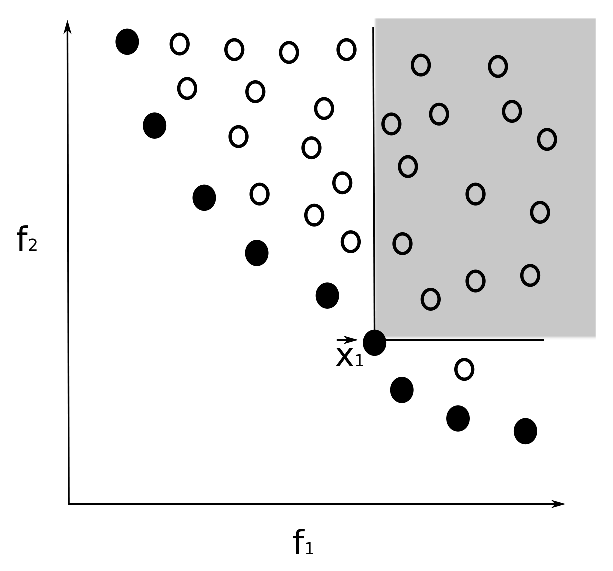
\includegraphics{Pareto2.eps}}
\end{minipage}
\caption{Σχηματική απεικόνιση της κυριαρχίας κατά \english{Pareto} σε πρόβλημα ελαχιστοποίησης δύο στόχων (Μ=2). Η λύση $\vec{x}_1$ είναι βέλτιστη κατά \english{Pareto} καθώς δεν κυριαρχείται από οποιαδήποτε άλλη λύση. Η λύση $\vec{x}_1$, αυτή καθαυτή, κυριαρχεί σε όλες τις λύσεις που υπάρχουν στη σκιασμένη περιοχή. Το μέτωπο των κατά \english{Pareto} βέλτιστων λύσεων, το οποίο εδώ απεικονίζεται με μαύρους κύκλους, δεν είναι υποχρεωτικά συνεχές.} 
\label{Pareto2}
\end{figure}

Ακολουθεί η παρουσίαση της τεχνικής $SPEA2$, \cite{Zitz02,Zitz01}, που χρησιμοποιείται για να μετατρέψει τα διανύσματα τιμών $F$ των μελών του τρέχοντος πληθυσμού σε βαθμωτές τιμές $\Phi$, με βάση την έννοια της κυριαρχίας κατά \english{Pareto}. Η $SPEA2$ αποδίδει σε κάθε άτομο μια βαθμωτή τιμή αντιπροσωπευτική της αλληλοκυριαρχίας των ατόμων της ένωσης των συνόλων $P_{\lambda}^g$, $P_{\mu}^g$ και $P_{e}^{g-1}$.   

\begin{itemize}
\item[]{\bf Βήμα 1:}  (Υπολογισμός δύναμης) Για κάθε μέλος ($i$) του πληθυσμού 
\newline
	$P=P_{\lambda}^g \cup P_{\mu}^g \cup P_{e}^{g-1}$
	υπολογίζεται η τιμή της δύναμης
		$S_i = \frac{\sum(j : j \in P \wedge i \prec j)} {\sum P}$. Σύμφωνα με τη σχέση αυτή, η δύναμη ενός μέλους $i$ ορίζεται ως το πλήθος των μελών του πληθυσμού στα οποία κυριαρχεί, διαιρεμένο με το συνολικό μέγεθος του πληθυσμού $P$.     

\item[]{\bf Βήμα 2:}  (Υπολογισμός πυκνότητας) Για κάθε μέλος $i$
	του πληθυσμού υπολογίζεται η τιμή πυκνότητας $D_i = \frac{1} {a_i+2}$, ως συνάρτηση της απόστασής του $a_i= min (\parallel \vec{F_i} - \vec{F_k} \parallel)$ από το κοντινότερο μέλος του πληθυσμού. 
	
\item[]{\bf Βήμα 3:}  (Υπολογισμός $\Phi$) 
Η βαθμωτή τιμή κόστους υπολογίζεται για κάθε άτομο του πληθυσμού και ορίζεται ως το άθροισμα
	$\Phi_i = R_i+D_i$
όπου 
\newline
$R_i=\sum _{j \in P \wedge i \prec j}|S_j|$ είναι μια βοηθητική ποσότητα (\english{raw fitness}) 
ίση με το άθροισμα της δύναμης των ατόμων από τα οποία κυριαρχείται το υπόψη άτομο. Μεγάλες τιμές της ποσότητας $R_i$ υποδηλώνουν ότι το άτομο κυριαρχείται από πολλά άλλα άτομα. Τα μέλη του μετώπου \english{Pareto} λαμβάνουν εξ ορισμού μηδενική τιμή ($R_i=0$).
\end{itemize}


\subsection{Βελτιστοποίηση με Περιορισμούς}
\label{COPini}
Στην πλειονότητα τους, τα προβλήματα βελτιστοποίησης, κυρίως αυτά που αφορούν σε βιομηχανικές εφαρμογές, πρέπει να ικανοποιούν και ένα σύνολο περιορισμών. Οι περιορισμοί μπορεί να σχετίζονται με γεωμετρικά χαρακτηριστικά ή λειτουργικές επιδόσεις λ.χ. της σχεδιαζόμενης στροβιλομηχανής.  Σε αυτήν τη διατριβή, οι 
ΕΑ 
\newline
αντιμετωπίζουν τα προβλήματα με περιορισμούς κάνοντας χρήση συναρτήσεων ποινής (\english{penalty functions} \cite{Deb00,morales98}).   

Οι όροι ποινής είναι ανάλογοι του κατά πόσο παραβιάζεται ο κάθε περιορισμός και προστίθενται στην $\Phi$. Για κάθε περιορισμό, εκτός της τιμής του κατωφλίου $d_k$ της σχέσης \ref{OptimIN}, ορίζεται επιπλέον και μια «χαλαρωμένη» τιμή $d_k^*\!>\!d_k$. Στην περίπτωση που το άτομο υπερβεί το «χαλαρωμένο» κατώφλι $d_k^*$, τότε αυτομάτως αποδίδεται «ποινή θανάτου» (\english{death penalty}), η οποία πρακτικά ισοδυναμεί με «άπειρη» τιμή της ποσότητας $\Phi$. Στην περίπτωση που κανένας περιορισμός δεν υπερβαίνει το «χαλαρωμένο» όριο, η τιμή της $\Phi$ υπολογίζεται από τη σχέση:
     
\begin{eqnarray}
	\Phi(\vec{x})=\Phi(\vec{x})+ \prod _{k=1}^K{\left\{ 				\begin{array}{ll}
    exp(a_k\frac{c_k(x)-d_k}{d_k^* -d_k}) & ~~,c_k(x)>d_k\\
    1 & ~~,c_k(x)\leq d_k\end{array} \right. }
    \label{penal2}
\end{eqnarray}
όπου οι συντελεστές $a_k$ καθορίζονται από το χρήστη και ρυθμίζουν τη σημαντικότητα κάθε περιορισμού.


\begin{table}[htdp]
\centering
\begin{tabular}{lr} 
\hline
\hline
Πλήθος μεταβλητών σχεδιασμού & N\\
Πλήθος στόχων & M\\
Πλήθος περιορισμών   & K\\
\hline
Υποψήφια λύση, διάνυσμα μεταβλητών σχεδιασμού   & $\vec{x}=(x_1,...,x_N)$\\
Συνάρτηση-στόχος &$f_i(\vec{x})$ \\
Διάνυσμα στόχων (αν Μ$>\!1$)  &$\vec{F}=(f_1(\vec{x}),...,f_M(\vec{x}))$\\
Συνάρτηση-περιορισμός &$c_i(\vec{x})$ \\
Διάνυσμα περιορισμών  & $\vec{C}=(c_1(\vec{x}),...,c_K(\vec{x}))$\\
Βαθμωτή συνάρτηση κόστους & $\Phi$ \\
\hline
Πλήθος απογόνων ανά γενιά &   $\lambda$ 			\\
Πλήθος γονέων ανά γενιά&  $\mu$ 				\\
Πλήθος επιλέκτων ανά γενιά&  $e$			\\
Διάρκεια ζωής ατόμου (μετρούμενη σε γενιές)&  $\kappa$			\\
Πλήθος γονέων που σχηματίζουν έναν απόγονο &  $\rho$			\\
\hline
\hline
\end{tabular}
\caption{Γενικευμένος Εξελικτικός Αλγόριθμος $(\mu,\lambda)$EA: Βασικοί Συμβολισμοί.}
\label{GEA nomenclature} 
\end{table}



\section{ΕΑ Υποβοηθούμενοι από Μεταπρότυπα}
Η αντικατάσταση του ακριβούς προτύπου αξιολόγησης (λ.χ. του κώδικα ΥΡΔ στις εφαρμογές αερο- ή υδροδυναμικής) με κάποιο άλλο πρότυπο αξιολόγησης  (μεταπρότυπο/\english{metamodel}), το οποίο έχει αρκετά μικρότερο υπολογιστικό κόστος και, συνήθως, είναι μια γενική μέθοδος παρεμβολής ή προσέγγισης, είναι η βασική ιδέα των υποβοηθούμενων από μεταπρότυπα ΕΑ (\english{Metamodel-Assisted Evolutionary Algorithms} ή ΜΑΕΑ).

Σε αυτήν τη διατριβή χρησιμοποιούνται ΕΑ με μεταπρότυπα συνδεόμενα με την εξέλιξη μέσω της τεχνικής της προσεγγιστικής προ-αξιολόγησης (ΠΠΑ), \english{Inexact Pre--Evaluation (IPE)}, \cite{phd_Giotis,phd_Karakasis,phd_Kampolis,phd_Vera,LTT_2_018,LTT_2_044}. Η φάση της ΠΠΑ ξεκινά όταν στη βάση δεδομένων του ΕΑ έχει αρχειοθετηθεί ένας ελάχιστος αριθμός (ορίζεται από το χρήστη) αξιολογημένων υποψήφιων λύσεων.  Κατά τη φάση της ΠΠΑ, εκπαιδεύ-ονται $(\lambda\!-\!\lambda^*)$ μεταπρότυπα, όπου $\lambda^*$ ο αριθμός των ατόμων του τρέχοντος πληθυσμού που υπάρχουν ήδη στη βάση δεδομένων. Ασφαλώς,  αυτά τα $\lambda^*$ άτομα δεν χρειάζεται να αξιολογηθούν, για την απόδοση προσεγγιστικής τιμής κόστους $\Phi^*$ στις $(\lambda\!-\!\lambda^*)$ υποψήφιες λύσεις. Κάθε μεταπρότυπο δίνει μια εκτίμηση της τιμής της συνάρτησης-στόχου του αντίστοιχου ατόμου. Με αυτήν την έννοια, τα μεταπρότυπα χαρακτηρίζονται ως «τοπικά» (\english{local metamodels}). Τέλος, τα $\lambda_e$ καλύτερα άτομα του πληθυσμού, με βάση τις αποδοθείσες τιμές  $\Phi^*$, προκρίνονται για αξιολόγηση με το ακριβές πρότυπο, εδώ το λογισμικό ΥΡΔ. Λεπτομερέστερη περιγραφή της τεχνικής ΠΠΑ βρίσκεται στο Κεφάλαιο $2$ του πλήρους κειμένου. Το σχήμα \ref{MAEA} σκιαγραφεί ένα ΜΑΕΑ. 

\begin{figure}[h!]
\centering
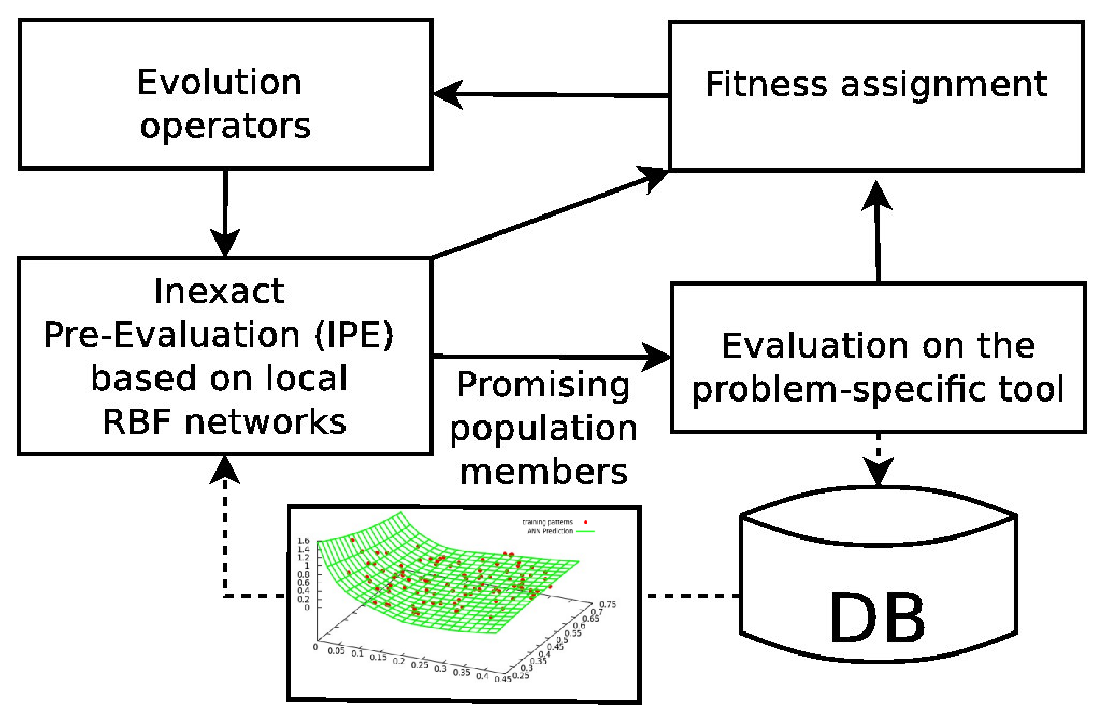
\includegraphics[width=100mm]{MAEA.eps} 
\caption{Ο ΜΑΕΑ με μεταπρότυπα συνδεδεμένα με την εξέλιξη μέσω της τεχνικής της προσεγγιστικής προ-αξιολόγησης (ΠΠΑ).}
\label{MAEA}
\end{figure}

Στην παρούσα διατριβή, ως μεταπρότυπα χρησιμοποιούνται τεχνητά νευρωνικά δίκτυα (ΤΝΔ, \english{Artificial Neural Networks, ANN)} και, συγκεκριμένα, Δίκτυα Συναρτήσεων Ακτινικής Βάσης \english{(Radial Basis Function networks, RBF)} \cite{Haykin}.

Ένα τυπικό δίκτυο \english{RBF}, με Ν εισόδους και μία έξοδο, κατάλληλο για την πρόβλεψη τιμής μιας συνάρτησης κόστους φαίνεται στο σχήμα \ref{rbf1}. Η συνάρτηση ενεργοποίησης που χρησιμοποιήθηκε είναι η $
	G(u,r)=exp(\frac{-u^2}{r^2})$  
όπου  $u=\Vert \vec{x}-\vec{c}_l \Vert_2$ είναι η απόσταση από το $l^{o}$ κέντρο $\vec{c}_l$ της συνάρτησης ακτινικής βάσης.

\begin{figure}[h!]
\centering
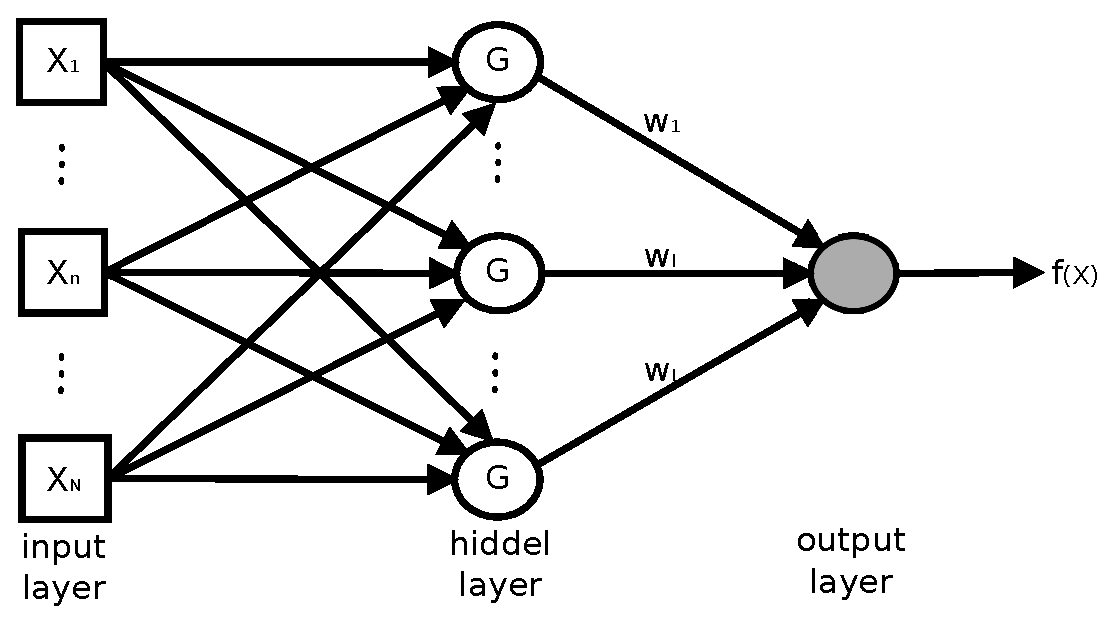
\includegraphics[width=100mm]{RBF.eps} 
\caption{Δίκτυο συναρτήσεων ακτινικής βάσης Ν εισόδων και μίας εξόδου, το οποίο χρησιμοποιείται ως μεταπρότυπο του ΜΑΕΑ της παρούσας διατριβής.}
\label{rbf1}
\end{figure}

%Η έξοδος του ΔΑΒ υπολογίζεται απο:
%\begin{eqnarray}
%	f(x)=\sum _1^K w_i*G(u(x_i),r)
%\label{response}
%\end{eqnarray}         
%\label{MAEApar}
%\newpage
\section{Ιεραρχική-Πολυεπίπεδη Βελτιστοποίηση} 

Η επίλυση ενός προβλήματος βελτιστοποίησης σε έναν αριθμό «επιπέδων βελτιστοποίησης», χρησιμοποιώντας στο κάθε επίπεδο: α) υπολογιστικά εργαλεία αξιολόγησης των υποψήφιων λύσεων διαφορετικού κόστους και ακρίβειας, β) μεθόδους ανίχνευσης διαφορετικού τύπου, ενδεχομένως στοχαστικές σε κάποια επίπεδα και αιτιοκρατικές σε άλλα, γ) παραμετροποίηση της προς σχεδιασμό μορφής με διαφορετικούς βαθμούς ελευθερίας,  αποτελεί τη βασική ιδέα της ιεραρχικής (\english{Hierarchical EA, HEA}) ή πολυεπίπεδης βελτιστοποίησης, \cite{phd_Kampolis,LTT_2_031,LTT_2_044,LTT_3_094,LTT_3_095}. 


Οι προαναφερθείσες μορφές ιεραρχικής-πολυεπίπεδης βελτιστοποίησης (σχήμα \ref{allheas}) μπορούν να χρησιμοποιηθούν ανεξάρτητα ή σε συνδυασμό, χρησιμοποιώντας δύο ή περισσότερα επίπεδα. 


\begin{figure}[h!]
    \centering
    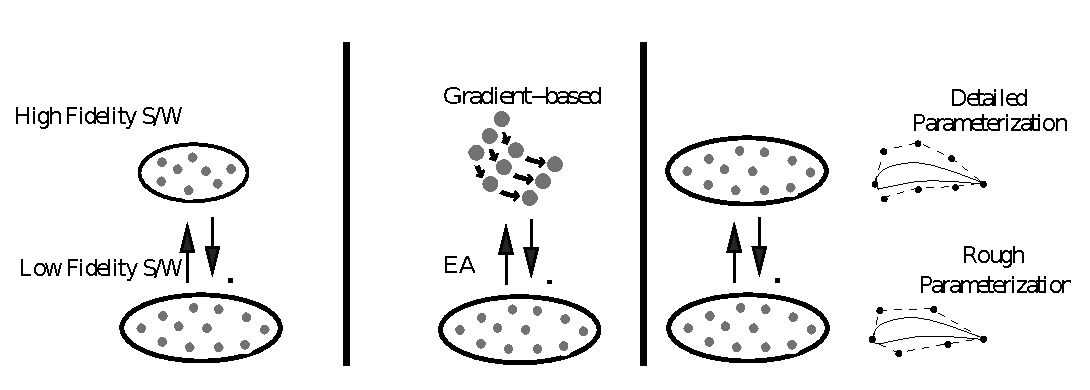
\includegraphics[scale=0.8]{multimodes.eps}
    \caption{Σχηματική απεικόνιση των τριών τύπων ιεραρχικής-πολυεπίπεδης βελτιστοποίησης. Παρουσιάζεται η πλέον συνηθισμένη διεπίπεδη μορφή του προαναφερθέντος γενικού τρόπου σε τρεις εναλλακτικές διατυπώσεις, \cite{phd_Kampolis}.}
    \label{allheas}
\end{figure}      

Στο σχήμα \ref{allheas}, αριστερά, απεικονίζεται ο πολυεπίπεδος (διεπίπεδος ΕΑ) με ιεραρχική αξιολόγηση (\english{Hierarchical Evaluation}). Χρησιμοποιεί λογισμικό χαμηλού υπολογιστικού κόστους και πιστότητας στο χαμηλό επίπεδο και λογισμικό υψηλού κόστους και πιστότητας στο υψηλό επίπεδο, το οποίο χειρίζεται μικρότερο πληθυσμό. Στο μέσο, απεικονίζεται παραλλαγή βασισμένη στην ιεραρχική ανίχνευση (\english{Hierarchical Search}) που υλοποιείται συνήθως εφαρμόζοντας ΕΑ στο χαμηλό επίπεδο και αιτιοκρατικές μεθόδους βελτιστοποίησης στο υψηλό επίπεδο. Τέλος, δεξιά, απεικονίζεται μια τρίτη παραλλαγή που βασίζεται στην ιεραρχική παραμετροποίηση (\english{Hierarchical Parameterization}). Αυτή συνδυάζει την αδρή παραμετροποίηση της προς σχεδιασμό μορφής με λίγες μεταβλητές σχεδιασμού στο χαμηλό επίπεδο με τη λεπτομερή παραμετροποίησή της, με όλους τους βαθμούς ελευθερίας, στο υψηλό επίπεδο.

Η ιεραρχική βελτιστοποίηση δεν χρησιμοποιείται στις εφαρμογές που παρουσιάζει η διατριβή αυτή. Η χρήση των εδώ προτεινόμενων τεχνικών μείωσης του υπολογιστικού κόστους είναι, όμως, άμεσα επεκτάσιμη και στην περίπτωση που χρησιμοποιείται ιεραρχικός ΕΑ. Το κέρδος από τις νέες μεθόδους αναμένεται να υπερτίθεται σε αυτό των ιεραρχικών ΕΑ.



%--------------------------------------------------------------------------
% ----------------------- end of thesis sub-document ------------------------
% ---------------------------------------------------------------------------					% EAs
% this file is called up by thesis.tex
% content in this file will be fed into the main document
\chapter{Σχεδιασμός στη Βάση Αρχειοθετημένης Γνώσης} % top level followed by section, subsection
%: ----------------------- paths to graphics ------------------------

% change according to folder and file names
\ifpdf
    \graphicspath{{3/figures/PNG/}{3/figures/PDF/}{2.5/figures/}}
\else
    \graphicspath{{3/figures/EPS/}{3/figures/}}
\fi

%: ----------------------- contents from here ------------------------
Σε αυτό το κεφαλαίο προτείνεται, υλοποιείται και αξιολογείται μια πρωτότυπη διαδικασία σχεδιασμού στροβιλομηχανών η οποία εκμεταλλεύεται τη διαθεσιμότητα  παλαιότερων αρχειοθετημένων σχεδιασμών. Οι τελευταίοι θεωρούνται βέλτιστοι ή πολύ ικανοποιητικοί για λειτουργία σε διαφορετικές μεν, αλλά «συναφείς» συνθήκες. Αυτή η διαδικασία θα ονομάζεται σχεδιασμός στη βάση αρχειοθετημένης γνώσης ή \english{Knowledge Based Design (KBD),} \cite{Kyriacou2010}. Αν και  το υλικό που παρουσιάζεται περιορίζεται σε περιπτώσεις στροβιλομηχανών, η μέθοδος είναι γενική και άμεσα εφαρμόσιμη σε οποιαδήποτε άλλη επιστημονική περιοχή.    

Η προτεινόμενη διαδικασία σχεδιασμού αποτελεί ένα πρωτότυπο συνδυασμό της γενικότερης μεθόδου «Αιτιολογίας Κατά Περίπτωση» \english{(Case Based Reasoning, CBR)}, \cite{kolodner_1991,slade_1991,riesbeck_1989}, που εντάσσεται στην κατηγορία «Συστημάτων Αρχειοθετημένης Γνώσης» \english{(Knowledge Based Systems, KBS)} και των ΕΑ. Η προτεινόμενη \english{KBD} αποτελεί μία εντελώς αυτοματοποιημένη διαδικασία, από τη στιγμή που έχουν επιλεγεί οι αρχειοθετημένοι σχεδιασμοί (σχεδιασμοί βάσης) και δεν απαιτεί παρέμβαση του χρήστη κατά τη διαδικασία αναθεώρησης της προτεινόμενης λύσης, όπως αυτό συμβαίνει στη συμβατική \english{CBR}. 
Το επιδιωκόμενο αποτέλεσμα θα μπορούσε, εν μέρει, να επιτευχθεί με απλή ένταξη των αρχειοθετημένων σχεδιασμών στην πρώτη γενιά του ΕΑ, μαζί με κατάλληλο καθορισμό των ορίων των μεταβλητών σχεδιασμού. Αντ' \newline αυτού, στην προτεινόμενη διαδικασία, χρησιμοποιούνται τεχνικές στατιστικής ανάλυσης έτσι ώστε να επιτευχθεί περαιτέρω επιτάχυνση του ΕΑ. Η προτεινόμενη διαδικασία \english{KBD} επιτυγχάνει:           

\begin{description}
  \item[α)] Αισθητή μείωση των μεταβλητών σχεδιασμού που χειρίζεται ο ΕΑ, επιφέροντας σημαντική επιτάχυνση της βελτιστοποίησης. Ουσιαστικά, επιτυγχάνει τον ε-ντοπισμό της/των βέλτιστης/ων λύσης/εων με μικρότερο αριθμό κλήσεων του λογισμικού αξιολόγησης. Επιπλέον, προκαλεί ακόμη μεγαλύτερη επιτάχυνση λόγω της αύξησης του κέρδους από τη χρήση μεταπροτύπων. Στην προτεινόμενη μέθοδο, τα μεταπρότυπα εκπαιδεύονται αποκτώντας μεγαλύτερη ακρίβεια πρόβλεψης ενώ η διαδικασία της ΠΠΑ μπορεί να εκκινεί νωρίτερα, με αρκετά λιγότερα πιθανά δείγματα εκπαίδευσης στη βάση δεδομένων την οποία διατηρεί και ανανεώνει ο ΕΑ, κατά την εξέλιξή του.   
  \item[β)] Τον αυτόματο/άκοπο καθορισμό των ορίων των μεταβλητών σχεδιασμού, απαλλάσσοντας έτσι το σχεδιαστή από τη διαδικασία επιλογής τους και εξαλείφο-ντας παράλληλα τον κίνδυνο λάθους (η βέλτιστη λύση να βρίσκεται έξω από τα όρια των μεταβλητών σχεδιασμού). Υπενθυμίζεται ότι η βελτιστοποίηση μέσω ΕΑ προαπαιτεί τον καθορισμό άνω και κάτω ορίων τιμών για κάθε μεταβλητή. 
    \item[γ)] Τη δυνατότητα αντιστοίχισης τιμών σημαντικότητας στις περιοχές του χώρου σχεδιασμού, όπως αυτές υπολογίζονται από τη στατιστική ανάλυση των αρχειοθετημένων σχεδιασμών. Η απόδοση υψηλής σημαντικότητας σε μια υποπεριοχή του χώρου σχεδιασμού μετουσιώνεται σε μεγαλύτερη πιθανότητα δημιουργίας απογόνων σε αυτήν, κατά τη διαδικασία της εξέλιξης.
\end{description}

Οι προαναφερθείσες ιδιότητες της \english{KBD} επιτρέπουν την αποδοτική ανίχνευση μεγάλων χώρων σχεδιασμού, τόσο ως πρός το πλήθος των μεταβλητών σχεδιασμού όσο και ως προς το εύρος αυτών,  εκμεταλλευόμενη την πληροφορία/γνώση που ενυπάρχει στους αρχειοθετημένους σχεδιασμούς.  


\section{Διατύπωση Νέου Σχεδιασμού}
Στην προτεινόμενη μέθοδο, ο τρόπος διατύπωσης κάθε νέου σχεδιασμού είναι άρρηκτα συνδεδεμένος με την εισαγωγή των λεγόμενων μεταβλητών βελτιστοποίησης (\english{optimization variables}). Οι μεταβλητές βελτιστοποίησης αποτελούν ένα διαφορετικό σύνολο μεταβλητών σχεδιασμού, μικρότερης κατά κανόνα διάστασης από αυτό που προκύπτει από την κλασική παραμετροποίηση μορφής. Στη μέθοδο \english{KBD}, οι άγνωστοι του προβλήματος θα ονομάζονται σκόπιμα «μεταβλητές βελτιστοποίησης»  για να υπάρξει αντιδιαστολή ως προς τις «μεταβλητές σχεδιασμού» που αντιστοιχούν στην κλασική παραμετροποίηση μορφής. Στην τελευταία περίπτωση, λ.χ. μεταβλητές σχεδιασμού θα μπορούσαν να είναι οι συντεταγμένες των σημείων ελέγχου συναρτήσεων \english{Bezier} κ.ο.κ.        

Η διαδικασία εισαγωγής των μεταβλητών βελτιστοποίησης έχει ως αφετηρία τους $m$ σχεδιασμούς βάσης ($m$ αρχειοθετημένα πτερύγια, αν λ.χ. σχεδιάζεται ένα νέο πτερύγιο στροβιλομηχανής). Αυτά θα συμβολίζονται ως $GEO_i=(x_1^i,x_2^i,....,x_N^i)$, $i\!=\!1,...,m$ όπου $x_j$, $j=1,...,N$ οι μεταβλητές σχεδιασμού όπως αυτές προκύπτουν από την παραμετροποίηση μορφής. Θεωρείται ότι οι $m$ σχεδιασμοί βάσης περιγράφο-νται όλοι με την ίδια παραμετροποίηση. Σε διαφορετική περίπτωση, επαφίεται στο σχεδιαστή να δημιουργήσει κοινή παραμετροποίηση. Αυτό μπορεί να γίνει λ.χ. μέσω ΕΑ αλλά το θέμα ξεφεύγει από το πλαίσιο της παρούσας διατριβής.     

Στη συνέχεια, υπολογίζονται οι μέσες τιμές ($\mu _j$) και οι τυπικές αποκλίσεις ($\sigma _j$) όλων των μεταβλητών σχεδιασμού των $m$ σχεδιασμών βάσης. Συμβολικά,
  
\begin{eqnarray}
		\left( {\begin{array}{c}
 		x_1^1  \\
 		\vdots  \\
 		x_N^1	\\
 		\end{array} } \right) 
 		\left( {\begin{array}{c}
 		x_1^i  \\
 		\vdots  \\
 		x_N^i	\\
 		\end{array} } \right)
 		\left( {\begin{array}{c}
 		x_1^m  \\
 		\vdots  \\
 		x_N^m	\\
 		\end{array} } \right) \rightarrow
		\left( {\begin{array}{c}
 		\mu _1  \\
 		\vdots  \\
 		\mu _N  \\
 		\end{array} } \right)
		\left( {\begin{array}{c}
 		\sigma _1  \\
 		\vdots  \\
 		\sigma _N  \\
 		\end{array} } \right)
   \label{cdf-matrix} 
\end{eqnarray}

Οι Ν μεταβλητές σχεδιασμού ομαδοποιούνται σε Κ ομάδες. Τα κριτήρια για την ομαδοποίηση μπορεί να είναι πολλά. Συνήθως, αλλά όχι αναγκαστικά, όλες οι μεταβλητές σχεδιασμού που αναφέρονται στην ίδια συνιστώσα της προς σχεδιασμό γεωμετρίας εντάσσονται στην ίδια ομάδα. Ενδεικτικά, κατά το σχεδιασμό λ.χ. μιας πτερύγωσης στροβιλομηχανής, οι μεταβλητές σχεδιασμού που παραμετροποιούν τη γενέτειρα του κελύφους ποδός συνήθως ανήκουν στην ίδια ομάδα, αυτές της γενέτειρας κελύφους κεφαλής σε μια άλλη, μια τρίτη ομάδα μπορεί να αποτελείται από τις μεταβλητές που σχετίζονται με τη μέση επιφάνεια κυρτότητας του πτερυγίου, κ.ο.κ. 

Στη σχέση που ακολουθεί εισάγονται συντελεστές βάρους $w_{i,k}$, όπου ο δεύτερος δείκτης αφορά στην ομάδα ($k=1,...,K$) στην οποία εντάχθηκε η αντίστοιχη μεταβλητή σχεδιασμού $x_j$. Κάθε νέος σχεδιασμός (άρα και ο ζητούμενος βέλτιστος) προκύπτει ως 

\begin{eqnarray}
   x_j^{new} = \Phi _j^{-1} (\frac{\sum_{i=1}^{m}w_{i,k} \Phi _j(x_j^i)}{\sum_{i=1}^{m}w_{i,k} }) 
   \label{non-linear2} 
\end{eqnarray}
όπου $\Phi_j$ η σιγμοειδής αθροιστική συνάρτηση κανονικής κατανομής για την $j$, δηλαδή η

\begin{eqnarray}
   \Phi _{j} (x)= \frac{1}{\sigma _j\sqrt[2]{2\pi}}\int _{-\infty}^x exp(\frac{-(u-\mu _j)^2}{2 \sigma _j^2 })du 
   \label{cdf} 
\end{eqnarray}
ενώ τα $\sigma _j$ και $\mu _j$ υπολογίζονται από τη σχέση \ref{cdf-matrix}. Στο σημείο αυτό αξίζει να τονισθεί η διάκριση στα χρησιμοποιούμενα σύμβολα. Υπενθυμίζεται ότι $x_j^i$ ($i=1,...,m$ και $j=1,...,N$) συμβολίστηκε η τιμή της $j$ μεταβλητής σχεδιασμού σύμφωνα με την παραμετροποίηση της  σχεδιαζόμενης μορφής για τον $i$-ιοστό σχεδιασμό βάσης. Αντι-θέτως, οι νέες μεταβλητές που θα χειριστεί ο ΕΑ («μεταβλητές βελτιστοποίησης») συμβολίζονται με $w_{i,k}$ και είναι $mK$ σε πλήθος. Σε αυτές, προστίθεται προαιρετικά μια ακόμη μεταβλητή, η $\Psi$.   
  
%Οι μεταβλητές βελτιστοποίησης που εισήχθησαν με αυτήν τη διαδικασία και τις οποίες τελικώς χειρίζεται ο ΕΑ, είναι τα βάρη ($w_{i,k}$, σχέση \ref{non-linear2}) τα οποία καθορίζουν τη συνεισφορά κάθε σχεδιασμού βάσης, ανάλογα με την ομάδα στην οποία εντάχθηκε η εκάστοτε μεταβλητή σχεδιασμού, στο νέο σχεδιασμό. Ο πρώτος δείκτης $(i)$, στο βάρος $w_{i,k}$, σχετίζεται με το σχεδιασμό βάσης και ο δεύτερος δείκτης $(k)$ με την ομάδα στην οποία ανήκει η $(j)$ μεταβλητή σχεδιασμού.      

Η προαιρετική μεταβλητή προεκβολής ($\Psi$) δίνει την επιπλέον δυνατότητα δημιουργίας νέων σχεδιασμών και εκτός του εύρους $\mu _j \pm 3\sigma _j$, \cite{Kiemele}. Χρησιμοποιώντας τη μεταβλητή αυτή, τα $\sigma _j$  (που υπολογίστηκαν από τη \ref{cdf-matrix}, τα οποία στη συνέχεια θα συμβολίζονται με $\sigma_j^{computed}$ για να διακρίνονται από τα τελικά $\sigma _j$ τα οποία θα  προκύψουν τελικά απο τη σχέση \ref{cdf-matrix-2})  υπολογίζονται από την          

\begin{eqnarray}
		\left( {\begin{array}{c}
 		\sigma _1  \\
 		\vdots  \\
 		\sigma _N  \\
 		\end{array} } \right) =
 		\Psi  
 		\left( {\begin{array}{c}
 		\sigma _1^{computed}  \\
 		\vdots  \\
 		\sigma _N^{computed}  \\
 		\end{array} } \right)
   \label{cdf-matrix-2} 
\end{eqnarray}
και είναι αυτά που θα χρησιμοποιηθούν για το σχηματισμό των νέων σχεδιασμών. 

Ο αριθμός των μεταβλητών βελτιστοποίησης που προκύπτει, ισούται με $m K+1$, συνυπολογίζοντας και την προαιρετική μεταβλητή  $\Psi$.


\section{Εφαρμογή: Σχεδιασμός 2Δ πτερύγωσης συμπιεστή}
\label{Drela1}
Η προτεινόμενη μέθοδος πιστοποιείται στο σχεδιασμό της αεροτομής 2Δ πτερύγωσης συμπιεστή. Η πτερύγωση λειτουργεί σε αριθμό \english{Mach} εισόδου $M_1=0.54$, γωνία εισόδου ροής$a_1=44^o$ και αριθμό \english{Reynolds} της ροής βασισμένο στη χορδή $c$ ίσο με $Re=4\times10^5$. Στόχος της βελτιστοποίησης είναι η ελαχιστοποίηση των απωλειών ολικής πίεσης $P_t$, στη μορφή του ομώνυμου συντελεστή   
\begin{eqnarray}
   \omega=\frac{p_{t1}-p_{t2}}{p_{t1}-p_1}
   \label{omegaLosses} 
\end{eqnarray}
όπου ο δείκτης $1$ υποδηλώνει την είσοδο ενώ ο δείκτης $2$ την έξοδο της πτερύγωσης.

Η προς σχεδιασμό αεροτομή υπόκειται σε γεωμετρικούς περιορισμούς που αφορούν στο ελάχιστο επιτρεπόμενο πάχος της σε διάφορες θέσεις. Στις θέσεις  $0.3c$, $0.6c$ και $0.9c$, όπου $c$ είναι το μήκος της αεροτομής, το ελάχιστο επιτρεπτό πάχος της αεροτομής είναι $0.10c$, $0.08c$ και $0.01c$, αντίστοιχα. Επίσης, η προς σχεδιασμό αεροτομή απαιτείται να προκαλεί στροφή της ροής $\Delta a= |a_2-a_1|$ μεγαλύτερη των $30^o$. Η παραμετροποίηση υλοποιείται χωριστά για τη μέση γραμμή κυρτότητας και την κατανομή πάχους και χρησιμοποιεί $27$ μεταβλητές σχεδιασμού. Κατά τον επιχειρούμενο με \english{KBD} σχεδιασμό, το διάνυσμα μεταβλητών σχεδιασμού χωρίζεται σε τρεις ομάδες ($K=3$) ως εξής: \english{i}) αυτές που ελέγχουν το σχήμα της μέσης γραμμής κυρτότητας \english{ii}) αυτές που ελέγχουν την κατανομή πάχους στην πλευρά υπερπίεσης και \english{iii}) αυτές που ελέγχουν την κατανομή πάχους στην πλευρά υποπίεσης. Στη διάθεσή του σχεδιαστή υπάρχουν $m=4$ αρχειοθετημένοι σχεδιασμοί που χρησιμοποιούνται ως γεωμετρίες βάσης. Τελικώς, οι μεταβλητές βελτιστοποίησης είναι $m K+1=13$ και αυτές, αντί των $27$, χειρίζεται ο ΕΑ. Λογισμικό αξιολόγησης είναι μια ολοκληρωματική μέθοδος επίλυσης των συνεκτικών στρωμάτων, σε συνδυασμό με επιλύτη των εξισώσεων \english{Euler} για την εξωτερική ροή, \cite{Drel1987}.          

Οι επιδόσεις των $m\!=\!4$ σχεδιασμών βάσης (σχήμα \ref{CBRarch}) στις επιθυμητές συνθήκες ροής μαζί με την προκαλούμενη στροφή της ροής έχουν ως εξής:  
\begin{itemize}
\item{Σχεδιασμός βάσης $Β_1$:} $\omega=0.0207$ και $\Delta a=36.3^o$.
\item{Σχεδιασμός βάσης $Β_2$:} $\omega=0.0278$ και $\Delta a=27.8^o$.
\item{Σχεδιασμός βάσης $Β_3$:} $\omega=0.0201$ και $\Delta a=37.5^o$.
\item{Σχεδιασμός βάσης $Β_4$:} $\omega=0.0237$ και $\Delta a=33.1^o$.
\end{itemize}
 
\begin{figure}[h!]
\begin{minipage}[b]{1\linewidth}
 \centering
 \resizebox*{14cm}{!}{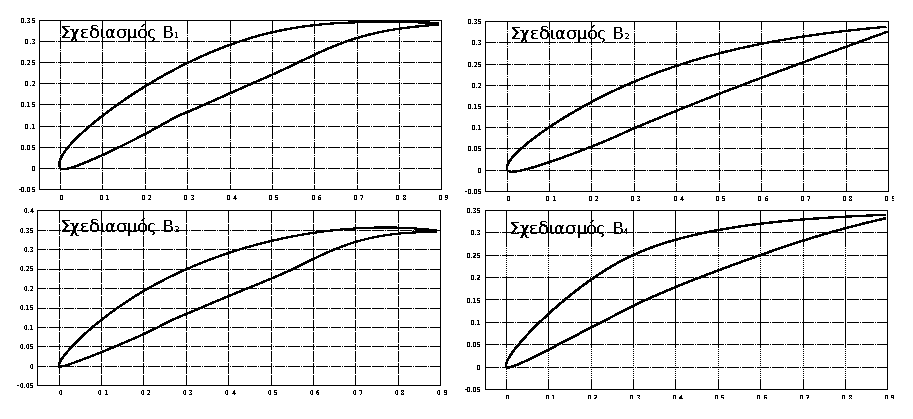
\includegraphics{blade_s.eps}}
\end{minipage}
\caption{Σχεδιασμός 2Δ πτέρυγωσης συμπιεστή: Οι $4$ αεροτομές που  χρησιμοποιήθηκαν ως σχεδιασμοί βάσης κατά την εφαρμογή της μεθόδου \english{KBD}, τοποθετημένες στην επιθυμητή γωνία κλίσης της πτερύγωσης.} 
\label{CBRarch}
\end{figure}

Παρατηρείται ότι και οι $4$ σχεδιασμοί βάσης, όταν χρησιμοποιηθούν στις επιθυμητές συνθήκες ροής αντί των συνθηκών για της οποίες είχαν σχεδιαστή (περιγράφο-νται στο πλήρες κείμενο), έχουν σχετικά μεγάλες τιμές απωλειών $\omega$. Επιπροσθέτως, ο σχεδιασμός β, δεν σέβεται τον περιορισμό στροφής της ροής. Και οι $4$ σχεδιασμοί βάσης σέβονται, από σύμπτωση ενδεχομένως, τους γεωμετρικούς περιορισμούς.    

Για τη μελέτη των επιδράσεων που έχει η χρήση της μεθόδου \english{KBD} τόσο στην εξέλιξη αυτή καθαυτή όσο και στη χρήση μεταπροτύπων κατά τη διαδικασία της βελτιστοποίησης, πραγματοποιήθηκαν $4$ ξεχωριστές διαδικασίες βελτιστοποίησης. Η πρώτη έκανε χρήση του κλασικού ΕΑ, η δεύτερη ενός ΕΑ υποβοηθούμενου από μεταπρότυπα (\english{MAEA}), η τρίτη ενός ΕΑ με \english{KBD} (\english{KBD-EA}) και, τέλος, η τέταρτη ενός \english{MAEA} με \english{KBD} (\english{KBD-MAEA}). Λεπτομερής περιγραφή των παραμέτρων εξέλιξης που χρησιμοποιήθηκαν υπάρχει στο πλήρες κείμενο της διατριβής, στο α-ντίστοιχο κεφάλαιο. Είναι όμως σημαντικό να αναφερθεί ότι οι $27$ μεταβλητές σχεδιασμού που χρησιμοποιήθηκαν στις δύο πρώτες μεθόδους, σύμφωνα με την παραμετροποίηση της γεωμετρίας με \english{NURBS}, έδωσαν τη θέση τους σε μόνο $13$ μεταβλητές βελτιστοποίησης κατά την εφαρμογή των δύο τελευταίων.   
Οι πορείες σύγκλισης των προαναφερθεισών διαδικασιών βελτιστοποίησης συγκεντρώνονται στο σχήμα \ref{CBRDrela}.           

\begin{figure}[h!]
\begin{minipage}[b]{1\linewidth}
 \centering
 \resizebox*{11cm}{!}{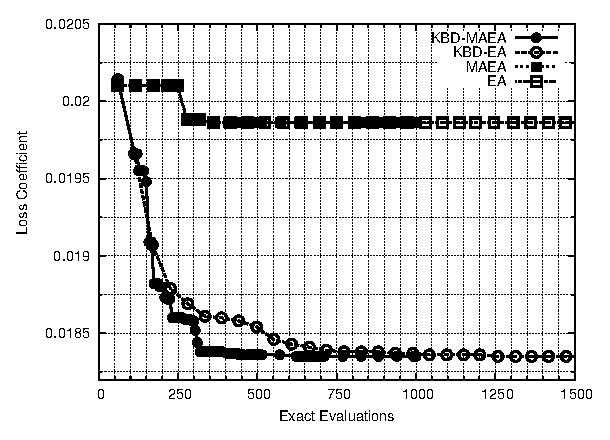
\includegraphics{Comp.eps}}
\end{minipage}
\caption{Σχεδιασμός 2Δ πτέρυγωσης συμπιεστή: Πορείες σύγκλισης των  ΕΑ, \english{MAEA}, \english{KBD-EA} και \english{KBD-MAEA}. Ο οριζόντιος άξονας αντιστοιχεί σε κλήσεις στο λογισμικό ΥΡΔ. Η εκπαίδευση των μεταπροτύπων έχει μηδενικό πρόσθετο κόστος. } 
\label{CBRDrela}
\end{figure}

Παρατηρείται ότι η χρήση μεταπροτύπων στον ΕΑ (ή ΜΑΕΑ) χωρίς επιπρόσθετη χρήση \english{KBD} δεν απέφερε κέρδος. Αυτό, κατά μεγάλο βαθμό, οφείλεται στο σχετικά πολύ μεγάλο εύρος του χώρου σχεδιασμού. Ακόμη, παρατηρείται η καθολική υπεροχή της μεθόδου \english{KBD-EA} συγκριτικά με τον κλασικό ΕΑ, αποδεικνύοντας έτσι την επιτάχυνση της εξέλιξης όταν χρησιμοποιούνται οι νέες μεταβλητές βελτιστοποίησης (μειωμένος αριθμός και εισαγωγή σημαντικότητας στις περιοχές του χώρου σχεδιασμού). Επίσης, παρατηρείται η επανεμφάνιση του «απωλεσθέντος» κέρδους λόγω της χρήσης μεταπροτύπων κατά τη διαδικασία της ΠΠΑ στον \english{KBD-MAEA}. Τα παραπάνω συνηγορούν στην αξία της μεθόδου \english{KBD}, είτε αυτή χρησιμοποιείται μαζί με τον ΕΑ ή το ΜΑΕΑ.            

Η βέλτιστη αεροτομή που υπολογίστηκε από τον \english{KBD-MAEA} παρουσιάζεται στο σχήμα \ref{CBRDrelaRes}. Έχει απώλειες ολικής πίεσης $\omega=0.01834$, τιμή αρκετά μικρότερη από όλους τους σχεδιασμούς βάσης. Επίσης ικανοποιεί όλους  του περιορισμούς και επιφέρει στροφή της ροής ίση με $\Delta a = 30.2^o$. 
%The optimal blade resulting form KBD-MAEA is presented in fig. \ref{CBRDrelaRes}. The design delivers $\omega=0.01834$ and $\Delta a = 30.2^o$ at the desirable conditions. The design is better than all basis design (operating at the desirable conditions) and respects all the constraints. The delivered form KBD-MAEA design is also of significantly better quality than the designs delivered by all the non-KBD optimization procedures. 


\begin{figure}[h!]
\begin{minipage}[b]{1\linewidth}
 \centering
 \resizebox*{14cm}{!}{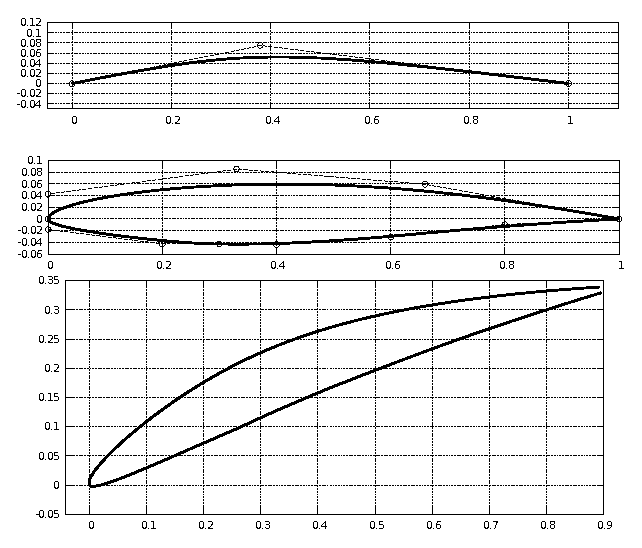
\includegraphics{ResD1.eps}}
\end{minipage}
\caption{Σχεδιασμός 2Δ πτέρυγωσης συμπιεστή: Η βέλτιστη αεροτομή η οποία υπολογίστηκε από τη μέθοδο \english{KBD-MAEA}. Η μέση γραμμή (πάνω) και οι κατανομές πάχους (κέντρο) για τις πλευρές υπερπίεσης και υποπίεσης, μαζί με τα πολύγωνα ελέγχου των πολυωνύμων \english{NURBS} που τις παρήγαγαν. Η βέλτιστη αεροτομή, τοποθετημένη στην επιθυμητή γωνία κλίσης της πτερύγωσης (κάτω). Η αεροτομή ικανοποιεί όλους τους τεθέντες περιορισμούς.} 
\label{CBRDrelaRes}
\end{figure}

%\begin{figure}[h!]
%\begin{minipage}[b]{1\linewidth}
% \centering
% \resizebox*{12cm}{!}{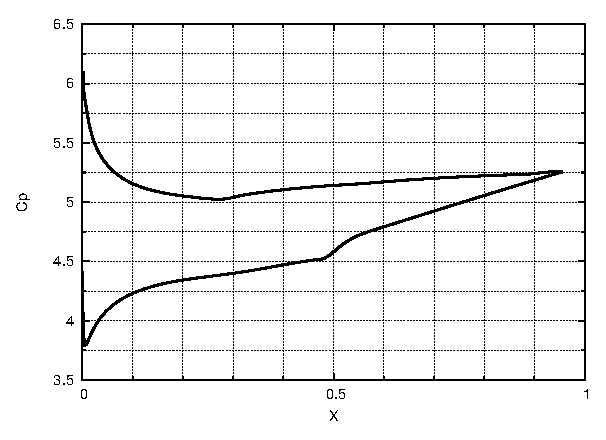
\includegraphics{Best_CP.eps}}
%\end{minipage}
%\caption{Συντελεστή πίεσης $C_p$ για την βέλτιστη αεροτομή της %εικόνας \ref{CBRDrelaRes}.} 
%\label{CBRDrelaRes_cp}
%\end{figure}


%
% ---------------------------------------------------------------------------
% ----------------------- end of thesis sub-document ------------------------
% ---------------------------------------------------------------------------
					% KBD
% change according to folder and file names
\ifpdf
    \graphicspath{{4/figures/PNG/}{4/figures/PDF/}{3/figures/}}
\else
    \graphicspath{{4/figures/EPS/}{4/figures/}}
\fi

%: ----------------------- contents from here ------------------------
\chapter{ΕΑ και ΜΑΕΑ Υποβοηθούμενοι από Ανάλυση Κυρίων Συνιστωσών } % top level followed by section, subsection
\label{VarCorrChapter}
%\begin{flushright}
%Any intelligent fool can make things  
%\linebreak
%bigger, more complex, and more violent. 
%\linebreak
%It takes a touch of genius, and a lot of  
%\linebreak
%courage, to move in the opposite direction.
%\linebreak
%Albert Einstein
%\end{flushright}
Το κεφάλαιο αυτό παρουσιάζει τρόπους με τους οποίους μπορεί να μειωθεί σημαντικά ο χρόνος βελτιστοποίησης με χρήση ΕΑ ή  παραλλαγών αυτών και, μάλιστα, υπερθετικά στη μείωση που επιφέρουν διάφοροι άλλοι ήδη γνωστοί τρόποι, όπως λ.χ. η προσεγγιστική προ-αξιολόγηση με μεταπρότυπα, κτλ.. Οι προτεινόμενοι τρόποι ενδείκνυνται για προβλήματα με μεγάλο αριθμό μεταβλητών σχεδιασμού και συνάρτηση κόστους $\Phi$ που είναι μη-διαχωρίσιμη (και ανισότροπη) ως προς τις μεταβλητές σχεδιασμού \cite{Salomon,Roy_2002a,Ghisu_2010}. Τα προβλήματα αυτά θα αναφέρονται ως «κακώς-τοποθετημένα» και προκαλούν μεγάλη καθυστέρηση στο ρυθμό σύγκλισης των ΕΑ ή των ΜΑΕΑ.  

Τα «κακώς-τοποθετημένα» προβλήματα έχουν σχέση με τον τρόπο που οι μεταβλητές σχεδιασμού ενός προβλήματος συσχετίζονται με συνάρτηση κόστους $\Phi$. Συνυφασμένες άμεσα με το πρόβλημα είναι οι έννοιες της ισότροπης ή μη-ισότροπης επίδρασης των μεταβολών τιμής των μεταβλητών σχεδιασμού στη μεταβολή τιμής της $\Phi$ και, κυρίως, του διαχωρίσιμου της. Η διαχείριση μιας μη-διαχωρίσιμης, μη-ισότροπης συνάρτησης-στόχου $\Phi$ κάνει το πρόβλημα βελτιστοποίησης «κακώς-τοποθετημένο». Τα μεγάλης διάστασης ($N»$) «κακώς-τοποθετημένα» προβλήματα βελτιστοποίησης χαρακτηρίζονται από μεγάλο κόστος επίλυσης μέσω των ΕΑ αλλά, ακόμη, και των ΜΑΕΑ. Επειδή δε τα περισσότερα βιομηχανικά προβλήματα ανήκουν σε αυτήν την κατηγορία, η επιθυμία για μείωση του κόστους επίλυσής τους είναι τεράστια.  Οι έννοιες της ισοτροπίας και του διαχωρίσιμου, καθώς και η επίδρασή τους στους ΕΑ, αναλύονται στην επόμενη ενότητα αυτού του κεφαλαίου. Από μαθηματικής σκοπιάς, ο εντοπισμός του τρόπου συσχέτισης της $\Phi$ με τις μεταβλητές σχεδιασμού υλοποιείται με την Ανάλυση σε Κύριες Συνιστώσες (ΑσΚΣ, \english{Principal Component Analysis \greek{ή} PCA}) \cite{Haykin}. Το κόστος χρήσης της ΑσΚΣ για τους σκοπούς του κεφαλαίου αυτού είναι το κόστος επίλυσης ιδιοπροβλημάτων μικρής διάστασης και κρίνεται, ως εκ τούτου, πάρα πολύ μικρό. Γίνεται, μάλιστα, αμελητέο όταν ο ΕΑ ή ο ΜΑΕΑ χρησιμοποιεί υψηλού κόστους λογισμικό αξιολόγησης των υποψήφιων λύσεων, όπως λ.χ. κώδικες ΥΡΔ.

Το κεφάλαιο αυτό προτείνει και πιστοποιεί, ως προς την αποδοτικότητα τους, δύο τρόπους εκμετάλλευσης των συσχετίσεων των μεταβλητών σχεδιασμού (ως προς τη $\Phi$) που εντοπίζει η ΑσΚΣ ή \english{PCA}. Ο πρώτος τρόπος σχετίζεται με την τροποποίηση των εξελικτικών τελεστών και θα αναφέρεται ως ΕΑ(\english{PCA}) ή ΜΑΕΑ(\english{PCA}) \cite{LTT_2_054}. Ο δεύτερος τρόπος σχετίζεται με τη χρήση μεταπροτύπων στο ΜΑΕΑ. Συγκεκριμένα, χρησιμοποιεί την πληροφορία που παρέχει η ΑσΚΣ κατά την ΠΠΑ των υποψήφιων λύσεων με μεταπρότυπα, ώστε τα τελευταία να εκπαιδεύονται με μικρό αριθμό σημαντικών εισόδων. Η μείωση αυτή του πλήθους εισόδων των μεταπροτύπων αυξάνει την αξιοπιστία τους, επιτρέπει τη χρήση τους νωρίτερα στο ΜΑΕΑ και επιφέρει υπολογιστικό κέρδος. Ο δεύτερος αυτός τρόπος θα αναφέρεται ως Μ(\english{PCA})ΑΕΑ. Στο ακρωνύμιο αυτό, ο προσδιορισμός \english{PCA} τοποθετείται μετά το Μ (Μ=\english{metamodel}, μεταπρότυπο) για να φανεί ακριβώς το που χρησιμοποιείται. Προφανώς, οι δύο τρόποι μπορούν να χρησιμοποιηθούν συνδυαστικά, σε μια νέα μέθοδο που θα αποκαλείται Μ(\english{PCA})ΑΕΑ(\english{PCA}).

Στο δεύτερο τμήμα του κεφαλαίου αυτού, οι προτεινόμενες τεχνικές πιστοποι-ούνται σε προβλήματα ελαχιστοποίησης κακώς-τοποθετημένων μαθηματικών συναρτήσεων. Στη συνέχεια, εκτίμηση του αναμενόμενου κέρδους γίνεται και σε ένα πρόβλημα σχεδιασμού-βελτιστοποίησης της μορφής της αεροτομής μιας 2Δ πτερύγωσης συμπιεστή. Βιομηχανικού ενδιαφέροντος εφαρμογές των προτεινόμενων μεθόδων παρουσιάζονται σε επόμενα κεφάλαια.             

 
%Σε αυτό το κεφάλαιο αρχικά παρουσιάζονται οι πιθανές ιδιαιτερότητες μιας συνάρτησης κόστους που ενδέχεται να προκαλέσουν συσχετίσεις μεταξύ των μεταβλητών σχεδιασμού (ΣΜΣ) \cite{Salomon,Roy_2002a,Ghisu_2010}. Στη συνέχεια, διερευνάται η επίδραση τους στους ΕΑ και αργότερα προτείνεται μία μέθοδος εντοπισμού αυτών των συσχετίσεων κάνονας χρήση Ανάλυσης σε Κύριες Συνιστώσες (ΑσΚΣ), \english{Principal Component Analysis (PCA)} και μέθοδοι αξιοποίησης τους αναβαθμίζοντας του τελεστές εξέλιξης. Προτείνεται, επίσης, η χρήση των ιδιοτιμών που υπολογίζονται από την ΑσΚΣ σαν μετρική σημαντικότητας των κατευθύνσεων στον χώρο σχεδιασμού και η αποκοπή των λιγότερο σημαντικών από αυτές κατά τη διαδικασία εκπαίδευσης του μεταπροτύπου.

%Τέλος οι προτεινόμενες τεχνικές πιστοποιούνται μέσα από αριθμό προβλημάτων μαθηματικής βελτιστοποίησης, ειδικά επιλεγμένων ούτως ώστε να εμπίπτουν στην κατηγορία των προβλημάτων με ΣΜΣ, και στον σχεδιασμό 2Δ πτερύγωσης συμπιεστή.
    
\section{Δυσκολίες λόγω Ιδιαιτερότητας της Συνάρτησης Κόστους}
Ένα πρόβλημα βελτιστοποίησης αναφέρεται ως «κακώς τοποθετημένο» αν παρουσιάζει συνδυασμό δύο ιδιαιτεροτήτων της συνάρτησης-κόστους $\Phi$ (σχήμα \ref{nonsep}): α) τη μη-ισότροπη συνεισφορά των μεταβλητών σχεδιασμού στη συνάρτηση κόστους και β) το μη-διαχωρίσιμο της $\Phi$.

Μη-ισότροπη συνεισφορά των μεταβλητών σχεδιασμού στη συνάρτηση-κόστους υπάρχει όταν ισόποσες μεταβολές των μεταβλητών σχεδιασμού δεν επιφέρουν ισόποσες μεταβολές στην τιμή της $\Phi$.  Μια συνάρτηση κόστους $\Phi$ ονομάζεται διαχωρίσιμη ως προς τη μεταβλητή σχεδιασμού $x_i$ αν η βέλτιστη τιμή του $x_i$ είναι ανεξάρτητη των τιμών των υπολοίπων μεταβλητών σχεδιασμού. Η $\Phi$ ονομάζεται διαχωρίσιμη αν είναι διαχωρίσιμη ως προς όλες τις μεταβλητές σχεδιασμού.        

\begin{figure}[h!]
\begin{minipage}[b]{1\linewidth}
 \centering
 \resizebox*{14cm}{!}{
\includegraphics{ellipseB.eps}}
\end{minipage}
%\begin{minipage}[b]{0.45\linewidth}
% \centering
% \resizebox*{9cm}{!}{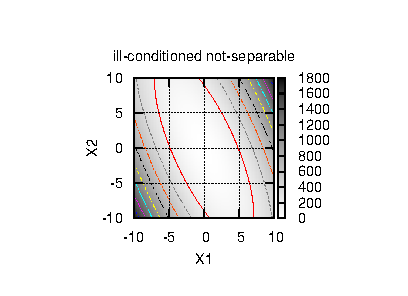
\includegraphics{ellipseturn.eps}}
%\end{minipage}
\caption{Πρόβλημα βελτιστοποίησης με μη-ισότροπη συνεισφορά των μεταβλητών σχεδιασμού στην $f$ (αριστερά). Πρόκειται για ισοϋψείς της $f$ της σχέσης \ref{ellipse} για Ν=2. Η μεταβλητή $x_2$ συνεισφέρει σε μεγαλύτερο βαθμό στην $f$ από ότι η $x_1$. Από την άλλη πλευρά, η $f$ είναι διαχωρίσιμη, άρα το πρόβλημα, ουσιαστικά δεν είναι «κακώς τοποθετημένο». Πρόβλημα βελτιστοποίησης με μη-ισότροπη συνεισφορά των μεταβλητών σχεδιασμού και μη-διαχωρίσιμες μεταβλητές σχεδιασμού ως προς την $f$ (δεξιά). Πρόκειται για ισοϋψείς της $f$ της σχέσης \ref{ellipse2} για Ν=2. Η βέλτιστη τιμή της $x_1$ εξαρτάται πλέον από τη $x_2$ και αντιστρόφως. Άρα, το πρόβλημα βελτιστοποίησης είναι πλέον «κακώς τοποθετημένο», κάτι που θα φανεί ιδιαίτερα λύνοντας το για μεγάλες τιμές του Ν.} 
\label{nonsep}
\end{figure}

Η επίδραση των παραπάνω χαρακτηριστικών στη συνάρτηση-στόχου $f$ σε ένα πρόβλημα βελτιστοποίησης, όταν αυτό επιλύεται με ΕΑ,  διερευνάται μέσω δύο προβλημάτων μαθηματικής βελτιστοποίησης επιλεγμένων ώστε να εμπίπτουν σε αυτήν την κατηγορία. Σκοπός της διερεύνησης είναι να δειχθεί ότι, αν το ίδιο πρόβλημα βελτιστοποίησης επαναδιατυπωθεί ως προς νέες μεταβλητές σχεδιασμού, ίδιου πλήθους, ως προς τις οποίες η υπόψη συνάρτηση κόστους είναι πλέον διαχωρίσιμη, ο ΕΑ εντοπίζει τη βέλτιστη λύση σε πολύ μικρότερο αριθμό αξιολογήσεων.  

Το πρώτο πρόβλημα αφορά ελαχιστοποίηση ενός πολυδιάστατου ελλειψοειδούς (η 2Δ μορφή του παρουσιάζεται στο σχήμα \ref{nonsep}). Η διαχωρίσιμη μορφή του περιγράφεται από τη σχέση   

\begin{eqnarray}
   \Phi=f(\vec{x})=\sum^{N}_{i=1}a^{\frac{i-1}{N-1}}x_i^2
   \label{ellipse} 
\end{eqnarray}
όπου $a$ είναι, πρακτικά, ο ο αριθμός κατάστασης της συνάρτησης. Μεγάλες τιμές της ποσότητας $a$ $(a>>1)$ ενισχύουν τη μη-ισότροπη συνεισφορά των μεταβλητών σχεδιασμού στην $f$.

Εναλλακτικά, μια μη-διαχωρίσιμη μορφή του ίδιου προβλήματος μπορεί να διατυπωθεί ως 
\begin{eqnarray}
   \Phi=f(\vec{x})=\sum^{N}_{i=1}a^{\frac{i-1}{N-1}}y_i^2
   \label{ellipse2} 
\end{eqnarray}
όπου $\vec{y}=B\vec{x}$ και $B$ ένα ($N\times N$) μητρώο στροφής. Η σύγκριση των σχέσεων \ref{ellipse} και \ref{ellipse2} φαίνεται εποπτικά, για Ν=2, στο σχήμα \ref{nonsep}. Ουσιαστικά, οι σχέσεις \ref{ellipse} και \ref{ellipse2} αναφέρονται στο ίδιο πρόβλημα ελαχιστοποίησης, με τη μορφή \ref{ellipse} να πλεονεκτεί της \ref{ellipse2} όταν η επίλυση γίνεται με ΕΑ ή ΜΑΕΑ.  

Η δεύτερη περίπτωση μαθηματικής βελτιστοποίησης αφορά στην ελαχιστοποίηση της πολυτροπικής (με πολλά τοπικά ακρότατα) συνάρτησης 

\begin{eqnarray}
  \Phi=f(\vec{x})=10N+(\sum^{N}_{i=1}x_i)^2 - 10Ncos(\pi  \sum^{N}_{i=1}x_i)
   \label{mm} 
\end{eqnarray}

Η συνάρτηση \ref{mm} αποτελεί τη μη-διαχωρίσιμη εκδοχή του προβλήματος βελτιστοποίησης. Η αντίστοιχη διαχωρίσιμη εκδοχή υπάρχει και προκύπτει, όμοια με την περίπτωση του ελλειψοειδούς, αν το $\vec{x}$ αντικατασταθεί απο το $\vec{y}$ όπου $\vec{y}=B\vec{x}$ και $B$ κατάλληλο μητρώο στροφής. Η συνάρτηση \ref{mm}, έχοντας, στην πραγματικότητα, μόνο μια σημαντική κατεύθυνση στο χώρο σχεδιασμού ($\sum^{N}_{i=1}x_i$), ανήκει στην κατηγορία των συναρτήσεων με εξαιρετικά μη-ισότροπη συνεισφορά των μεταβλητών σχεδιασμού στην $f$ (ως εάν $a=\infty$ στο προηγούμενο παράδειγμα). 
%Αυτή είναι μια πολύ σημαντική κατηγορία προβλημάτων γιατί προσομοιάζει σε συμπεριφορά τα προβλήματα βελτιστοποίησης πολλών στόχων, όπου στην πραγματικότητα μια περιοχή του χώρου των λύσεων εμπεριέχει όλους τους βέλτιστους σχεδιασμούς.           

Συγκριτικές πορείες σύγκλισης μεταξύ διαχωρίσιμης και μη-διαχωρίσιμης εκδοχής του $30$Δ ($N\!=\!30$) ελλειψοειδούς και της συνάρτησης \ref{mm} παρουσιάζονται στο σχήμα \ref{ellipse_t2}. Οι πορείες σύγκλισης απεικονίζουν μέσες τιμές υπολογισμένες για $10$ διαφορετικά τρεξίματα ΕΑ, με διαφορετική αρχικοποίηση της γεννήτριας τυχαίων αριθμών.  Παρατηρείται ότι, και στις δύο περιπτώσεις η διαχωρίσιμη εκδοχή των προβλημάτων υπερτερεί σημαντικά σε ταχύτητα της μη-διαχωρίσιμης εκδοχής αυτών. Το κέρδος  είναι σημαντικά μεγαλύτερο στην περίπτωση όπου $a=\infty$.        

\begin{figure}[h!]
%\begin{minipage}[b]{0.5\linewidth}
% \centering
% \resizebox*{7.5cm}{!}{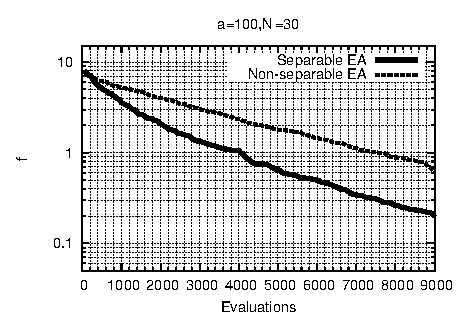
\includegraphics{100_30d.eps}}
%\end{minipage}
\begin{minipage}[b]{0.5\linewidth}
 \centering
 \resizebox*{7.5cm}{!}{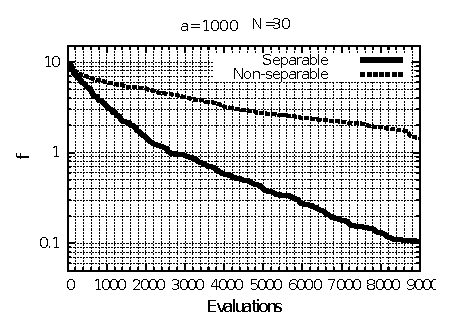
\includegraphics{1000_30db.eps}}
\end{minipage}
\begin{minipage}[b]{0.5\linewidth}
 \centering
 \resizebox*{7.5cm}{!}{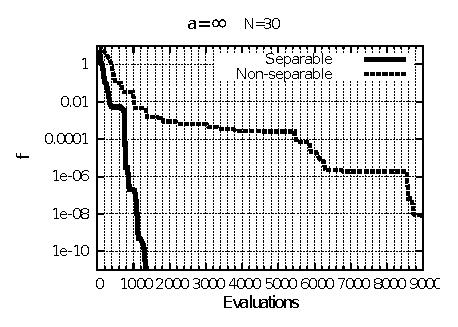
\includegraphics{30db.eps}}
\end{minipage}
\caption{Πορείες σύγκλισης ΕΑ για το 30Δ ελλειψοειδές με αριθμό κατάστασης (με $a=1000$) (αριστερά) και για την 30Δ συνάρτηση της σχέσης \ref{mm} (ως εάν $a=\infty$ στο προηγούμενο παράδειγμα) (δεξιά). Κάθε πρόβλημα λύνεται 10 φορές στη διαχωρίσιμη και άλλες 10 στη μη-διαχωρίσιμη εκδοχή του και σχεδιάζεται η μέση πορεία σύγκλισης κάθε εκδοχής.} 
\label{ellipse_t2}
\end{figure}



\section{Η Προτεινόμενη ΑσΚΣ}
Η προτεινόμενη μέθοδος κάνει χρήση της ΑσΚΣ για να υπολογίσει χρήσιμα τοπολογικά χαρακτηριστικά του συνόλου των επιλέκτων τα οποία και θεωρούνται αντιπροσωπευτικά των συσχετίσεων της $f$ ως προς τις μεταβλητές σχεδιασμού. Πιο αναλυτικά, αφού το σύνολο των επιλέκτων μετατραπεί σε ένα τυποποιημένο σύνολο δεδομένων Χ, \cite{Axler_1997}, δημιουργείται ο πίνακας συνδιακύμανσης $P_{N\times N}$ από τη σχέση 

\begin{equation} 
   P_{N\times N}= \frac{1}{e}XX^T
   \label{Cov_Mat} 
\end{equation}
όπου $e$ το πλήθος των επιλέκτων $P_e^g$ και $X$ ο πίνακας που έχει ως γραμμές τα διανύσματα σχεδιασμού που συνθέτουν το $P_e^g$ σε μορφή τυποποιημένου συνόλου δεδομένων.

Κάνοντας χρήση του φασματικού θεωρήματος αποσύνθεσης (\english{spectral decomposition theorem}),
 \cite{Axler_1997, Fodor_2002}, ο $P_{N\times N}$ μπορεί να γραφεί ως

\begin{equation} 
   P_{N\times N}= U\Lambda U^T
   \label{spectral}
\end{equation}
όπου $\Lambda\!=\!diag(\lambda_1 , . . . , \lambda_N )$ το διαγώνιο μητρώο των ιδιοτιμών και $U$ το $N\!\times\!N$ μητρώο των ιδιοδιανυσμάτων. 
Τα υπολογισθέντα ιδιοδιανύσματα (σχήμα \ref{reco1}) είναι οι κατευθύνσεις στο χώρο σχεδιασμού ως προς τις οποίες η $f$ είναι, κατά το δυνατό, διαχωρίσιμη. Αν ο ΕΑ χειριζόταν αγνώστους αναδιατυπωμένους σε αυτές τις κατευθύνσεις, το πρόβλημα βελτιστοποίησης θα μετατρεπόταν σε «λιγότερο  μη-διαχωρίσιμο» και, άρα, θα επιλυόταν με μικρότερο υπολογιστικό κόστος. Αυτήν την ιδέα υλοποιεί η προτεινόμενη μέθοδος.     

\begin{figure}[h!]
\begin{minipage}[b]{1\linewidth}
 \centering
 \resizebox*{!}{4.5 cm}{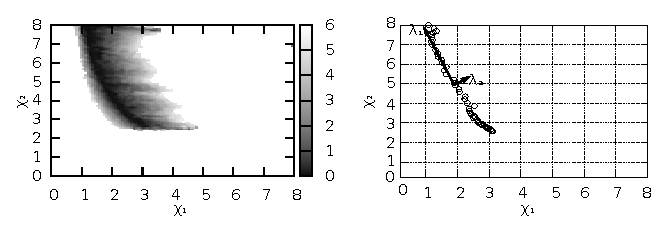
\includegraphics{DOFs.eps}}
\end{minipage}
\caption{Κατανομή της $f$ (ή της βαθμωτής $\Phi$ από λ.χ. τη διαδικασία \english{SPEA2}, για κάποια γενιά του ΕΑ, σε προβλήματα πολυκριτηριακής βελτιστοποίησης) στο χώρο σχεδιασμού (αριστερά). Το σύνολο των επίλεκτων $P^g_e$, για τη δεδομένη γενιά, και οι νέες κατευθύνσεις, στον χώρο σχεδιασμού,  $\lambda_1$ και $\lambda_2$, που ανέδειξε η ΑσΚΣ (αριστερά).} 
\label{reco1}
\end{figure}
       

\section{Εξελικτικοί Τελεστές Υποβοηθούμενοι από ΑσΚΣ} 

Με στόχο την επαναδιατύπωση του προβλήματος βελτιστοποίησης, χρησιμοποιώντας την πληροφορία που έδωσε  ΑσΚΣ για την υπόψη $f$, η παρούσα διατριβή προτείνει την εφαρμογή των τελεστών εξέλιξης (μετάλλαξης και διασταύρωσης), στο ευθυγραμμισμένο με τις νέες μεταβλητές σχεδιασμού που ανέδειξε η ΑσΚΣ. Με αυτήν την τακτική, η εξέλιξη λαμβάνει χώρα στο μετασχηματισμένο και κατά το δυνατό διαχωρίσιμο πρόβλημα βελτιστοποίησης, έχοντας σκοπό να ανακτήσει το (κατά το δυνατό) μεγαλύτερο ποσοστό απώλειας της απόδοσης του ΕΑ (σχήμα \ref{ellipse_t2}), που προκαλεί το μη-διαχωρισμό της $f$. Πληροφορίες σχετικές με τις ΣΜΣ προσδιορίζονται μέσω της ΑσΚΣ, η οποία επαναλαμβάνεται κάθε φορά που ένα νέο άτομο προστίθεται στο σύνολο των επιλέκτων. Η αξιοπιστία των υπολογιζόμενων ΣΜΣ ενισχύεται όσο το σύνολο των επιλέκτων προσεγγίζει το πραγματικό μέτωπο \english{Pareto}.              

%\begin{figure}[h!]
%\begin{minipage}[b]{1\linewidth}
% \centering
% \resizebox*{14cm}{!}{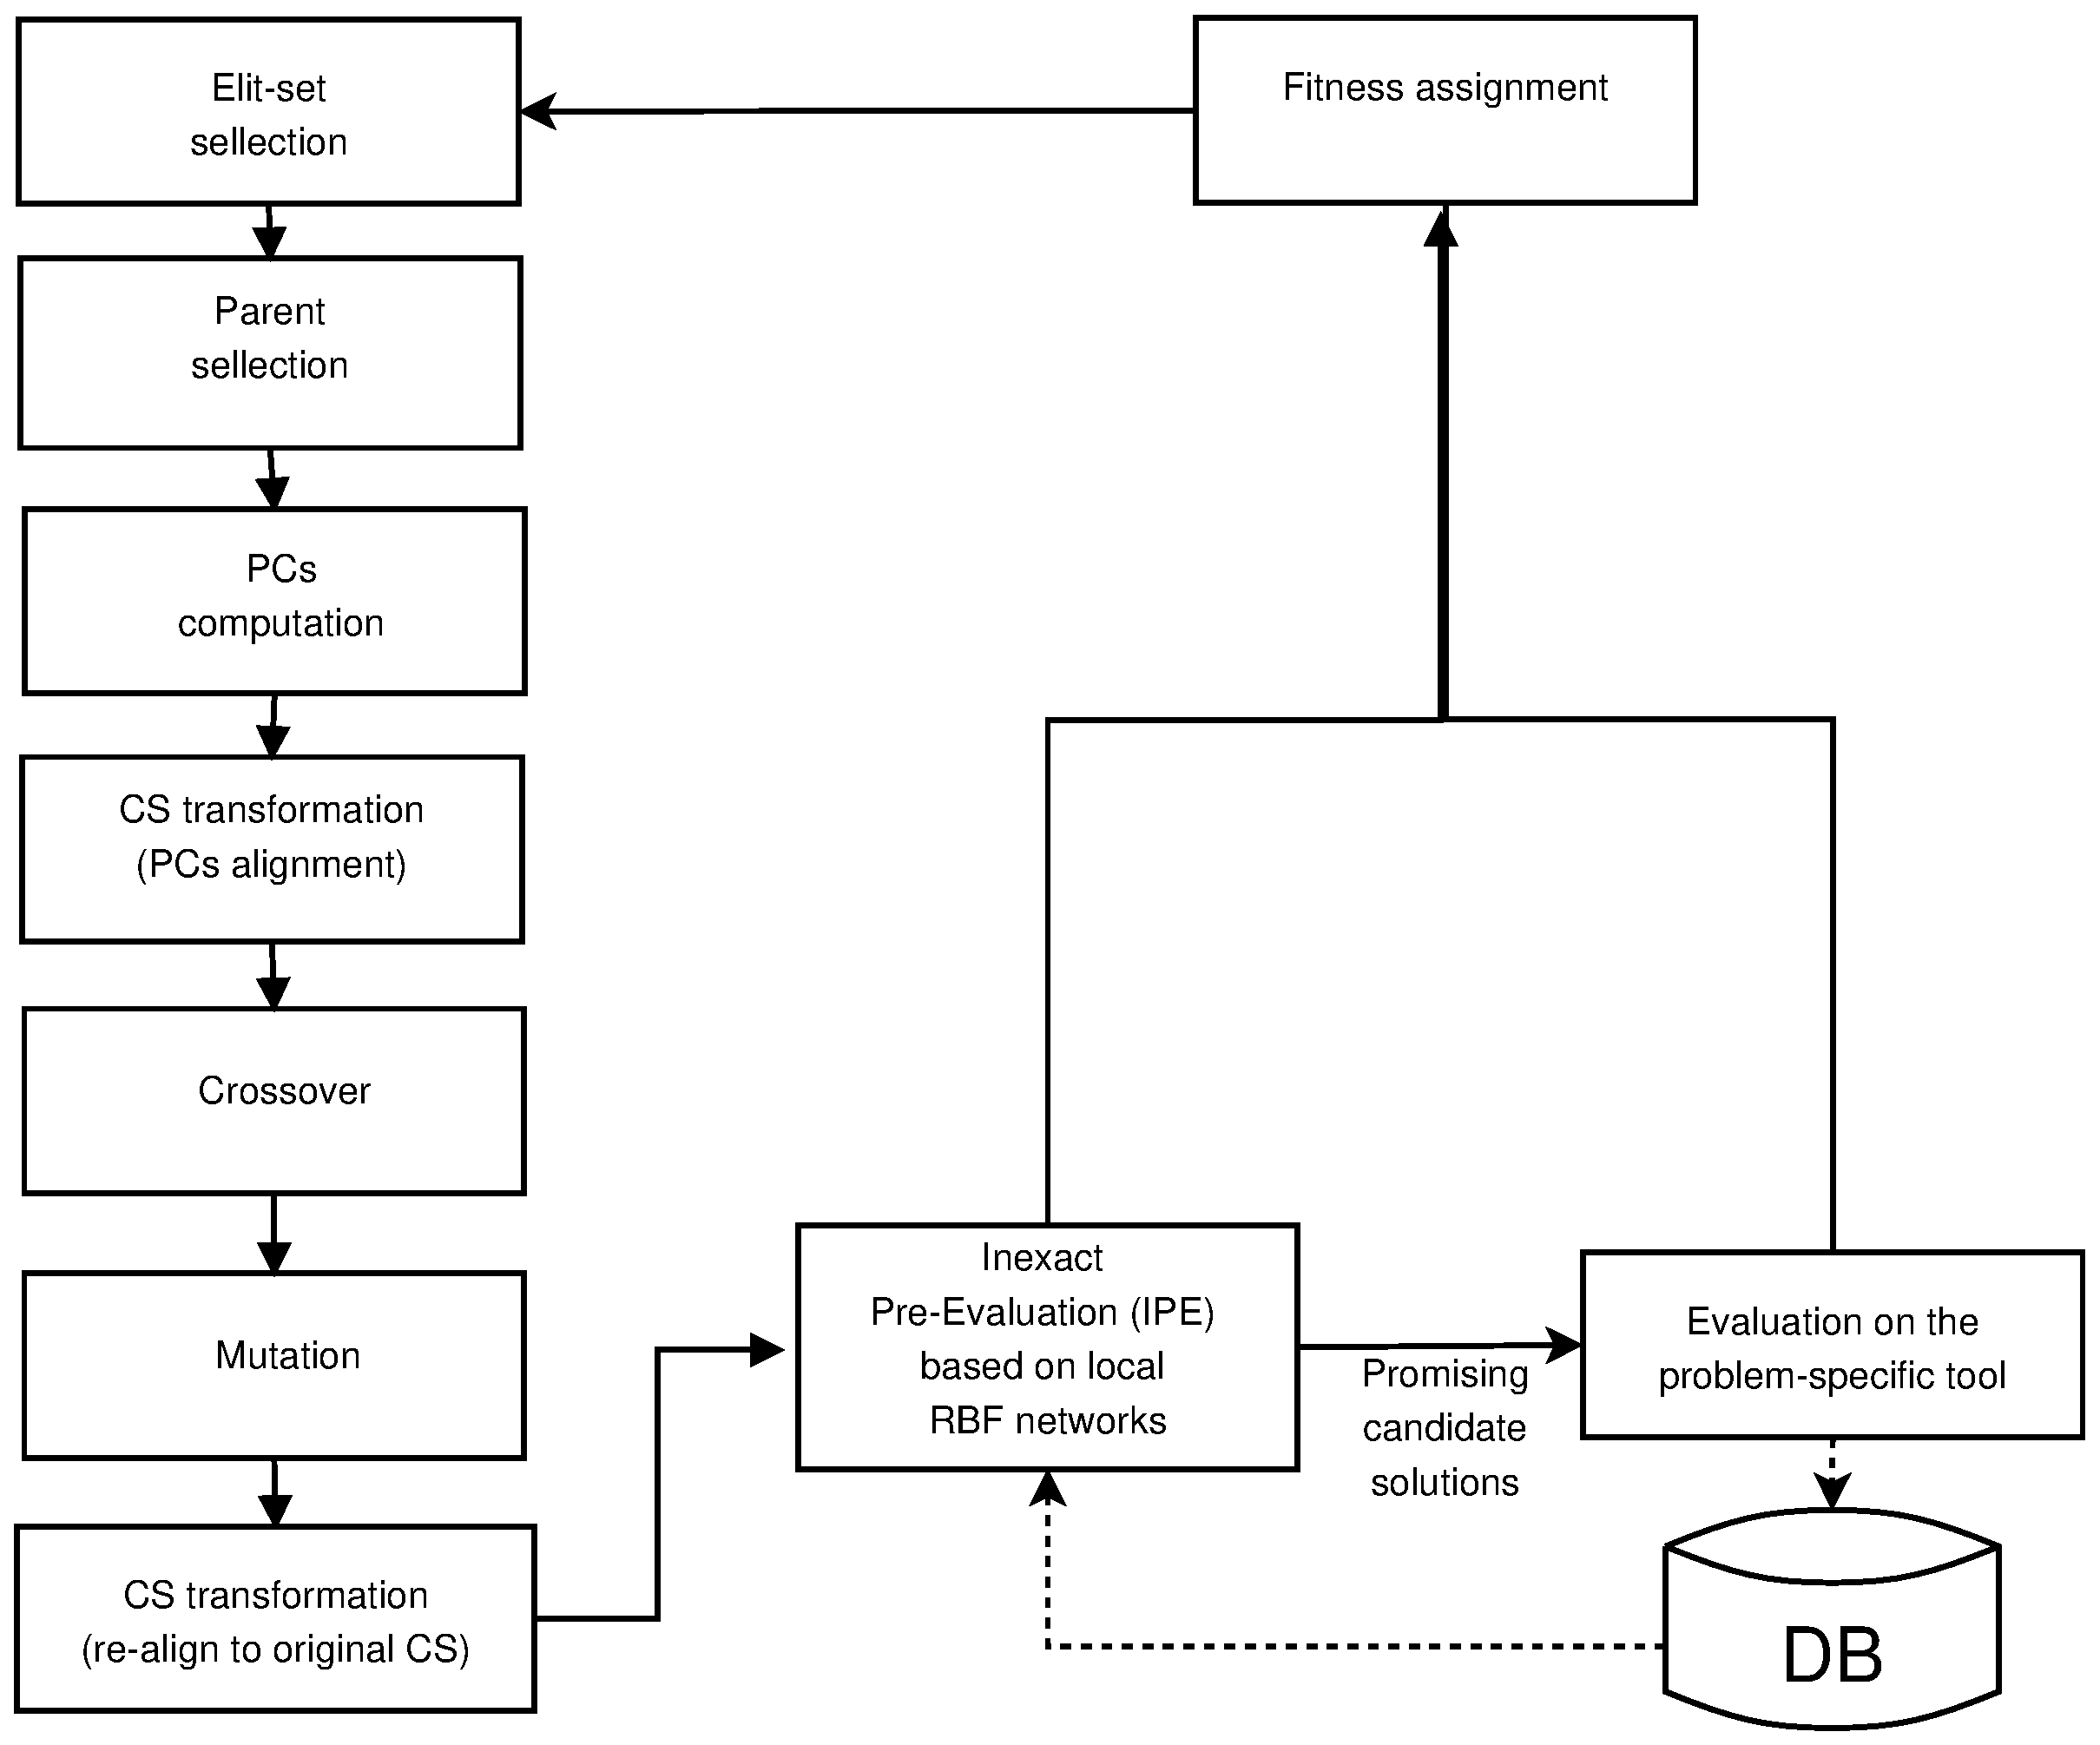
\includegraphics{MAEAPCA2.eps}}
%\end{minipage}
%\caption{Σχηματική απεικόνιση υποβοηθούμενου από μεταπρότυπα ΕΑ που κάνει χρίση τελεστών εξέλιξης υποβοηθούμενων από ΑσΚΣ (\english{MAEA(PCA)}).} 
%\label{MAEAPCA2}
%\end{figure}

\subsection{Πιστοποίηση εξελικτικών τελεστών υποβοηθού-μενων από ΑσΚΣ}
Το κέρδος απο τη χρήση των εξελικτικών τελεστών στις νέες μεταβλητές σχεδιασμού που ανέδειξε η ΑσΚΣ  ποσοτικοποιείται στα προβλήματα μαθηματικής ελαχιστοποίησης του 30Δ ελλειψοειδούς (σχέση \ref{ellipse}) και τις 30Δ πολυτροπικής συνάρτησης (σχέση \ref{mm}). 



\begin{figure}[h!]
%\begin{minipage}[b]{0.5\linewidth}
% \centering
% \resizebox*{7.5cm}{!}{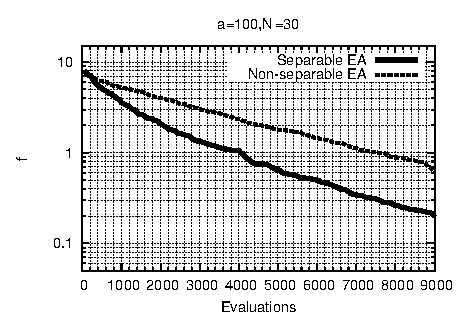
\includegraphics{100_30d.eps}}
%\end{minipage}
\begin{minipage}[b]{0.5\linewidth}
 \centering
 \resizebox*{7.5cm}{!}{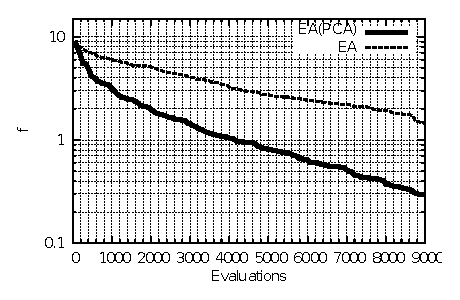
\includegraphics{1000_30d_pca.eps}}
\end{minipage}
\begin{minipage}[b]{0.5\linewidth}
 \centering
 \resizebox*{7.5cm}{!}{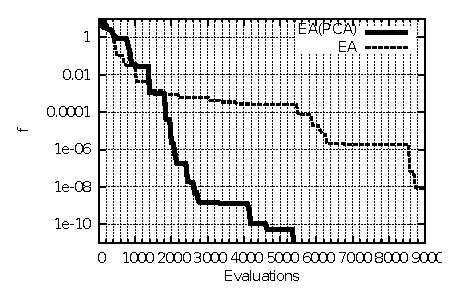
\includegraphics{30d_pca.eps}}
\end{minipage}
\caption{Πορείες σύγκλισης για το 30Δ ελλειψοειδές με αριθμό κατάστασης ($a\!=\!1000$) (αριστερά)  και την 30Δ συνάρτηση \ref{mm} (δεξιά). Η έντονη γραμμή παρουσιάζει την κατά πολύ βελτιωμένη σύγκλιση του ΕΑ στον οποίο οι εξελικτικοί τελεστές εφαρμόστηκαν στις εντοπιζόμενες από την ΑσΚΣ διαχωρίσιμες μεταβλητές σχεδιασμού.} 
\label{ellipse_t2_pca}
\end{figure} 

Οι πορείες σύγκλισης των ΕΑ και ΕΑ(\english{PCA}) για τις δύο αυτές συναρτήσεις παρουσιάζονται στο σχήμα \ref{ellipse_t2_pca}. Οι καμπύλες αποτελούν, και πάλι, τις μέσες τιμές των πορειών σύγκλισης που υπολογίσθηκαν τρέχοντας το ίδιο πρόβλημα $10$ φορές, κάθε φορά με διαφορετική αρχικοποίηση της γεννήτριας τυχαίων αριθμών.  Παρατηρείται ότι, και στα δύο προβλήματα, η χρήση των υποβοηθούμενων από την ΑσΚΣ τελεστών εξέλιξης υπερτερεί σημαντικά σε ταχύτητα και ανακτά ένα σημαντικό μέρος της μειωμένης απόδοσης των ΕΑ όταν αυτοί χρησιμοποιούνται για να λύσουν «κακώς τοποθετημένα» προβλήματα βελτιστοποίησης. 

\FloatBarrier
\section{Μεταπρότυπα Υποβοηθούμενα από ΑσΚΣ}
Η χρήση της ΑσΚΣ κατά τη διάρκεια εφαρμογής των τελεστών εξέλιξης δεν είναι η μόνη τεχνική που αποδείχθηκε ιδιαίτερα αποδοτική. Στην παρούσα διατριβή, προτείνεται επιπροσθέτως η χρήση των υπολογισθεισών, κατά την ΑσΚΣ, ιδιοτιμών ως μετρικών σημαντικότητας των κατευθύνσεων στο χώρο σχεδιασμού. Με τον τρόπο αυτό, η εκπαίδευση των μεταπροτύπων ενός ΜΑΕΑ πραγματοποιείται σε χώρο με αισθητά μειωμένη διάσταση. Τα μεταπρότυπα εκπαιδεύονται με μειωμένο αριθμό εισόδων, κρατώντας και χρησιμοποιώντας μόνο τις σημαντικότερες κατευθύνσεις στο χώρο σχεδιασμού που ανέδειξε η ΑσΚΣ και αποκόπτοντας τις λιγότερο σημαντικές. Η σημαντικότητα ορίζεται ως αντιστρόφως ανάλογη της ιδιοτιμής κάθε κατεύθυνσης στο χώρο σχεδιασμού.              



\begin{figure}
\begin{minipage}{0.48\textwidth}
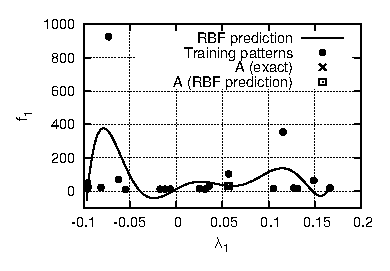
\includegraphics[scale=1.2]{IPE/f1_e1_b.eps}
\end{minipage}
\begin{minipage}{0.48\textwidth}
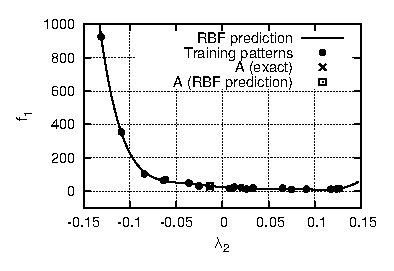
\includegraphics[scale=1.2]{IPE/f1_e2_b.eps}
\end{minipage}
\caption{ Εκτιμήσεις της τιμής της $f_1$ αν οι $\lambda_1$ (αριστερά) και $\lambda_2$ (δεξιά) χρησιμοποιηθούν, ξεχωριστά, ως είσοδοι του δικτύου \english{RBF}.}
\label{fig:f1e1e2}
\end{figure}

\begin{figure}
\begin{minipage}{0.48\textwidth}
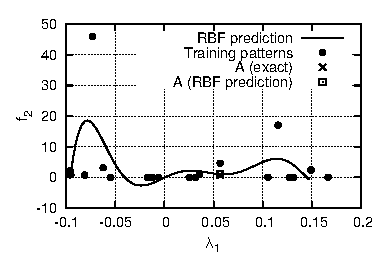
\includegraphics[scale=1.2]{IPE/f2_e1_b.eps}
\end{minipage}
\begin{minipage}{0.48\textwidth}
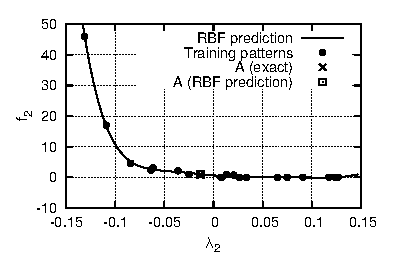
\includegraphics[scale=1.2]{IPE/f2_e2_b.eps}
\end{minipage}
\caption{Εκτιμήσεις της τιμής της $f_2$ αν οι $\lambda_1$ (αριστερά) και $\lambda_2$ (δεξιά) χρησιμοποιηθούν, ξεχωριστά, ως είσοδοι του δικτύου \english{RBF}.}
\label{fig:f2e1e2}
\end{figure}

%\begin{figure}[h!]
%\begin{minipage}[b]{0.5\linewidth}
% \centering
% \resizebox*{7.0cm}{!}{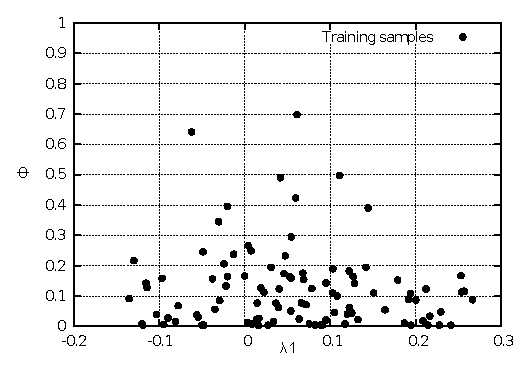
\includegraphics{1dANN_e1.eps}}
%\end{minipage}
%\begin{minipage}[b]{0.5\linewidth}
% \centering
% \resizebox*{7.0cm}{!}{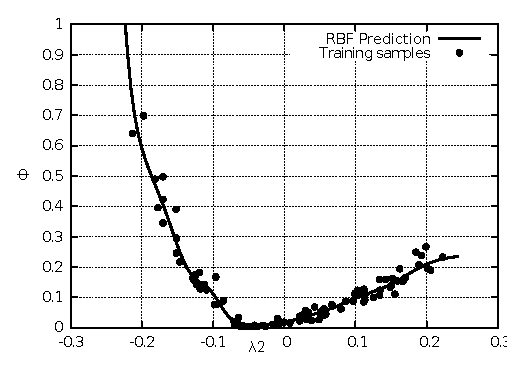
\includegraphics{1dANN_e2.eps}}
%\end{minipage}
%\caption{Εκτιμήσεις της τιμής της $\Phi$ από το μεταπρότυπο στο 2Δ πρόβλημα βελτιστοποίησης του σχήματος \ref{reco1}.  Πρότυπα εκπαίδευσης προβεβλημένα στο επίπεδο ($\Phi,\lambda_1$), όπου $\lambda_1$ η κατεύθυνση με τη μεγάλη ιδιοτιμή, βάσει της πραγματοποιηθείσας ΑσΚΣ (αριστερά). Πρότυπα εκπαίδευσης προβεβλημένα στο επίπεδο ($\Phi,\lambda_2$), όπου $\lambda_2$ η κατεύθυνση με τη μικρή ιδιοτιμή (δεξιά). Στην παρούσα διατριβή προτείνεται το μεταπρότυπo να εκπαιδευτεί μόνο στο  ($\Phi,\lambda_2$) επίπεδο, με το $\lambda_2$ δηλαδή ως τη μοναδική του είσοδο. Στο δεξιό σχήμα, με συνεχή γραμμή σχεδιάζεται η αναμενόμενη πρόβλεψη από το «σωστά» εκπαιδευμένο δίκτυο \english{RBF}. Στο αριστερό σχήμα, η αντίστοιχη καμπύλη αδυνατεί να παρακολουθήσει την ακατάστατη μορφή μορφή των αποκρίσεων και, για το λόγο αυτό, δεν σχεδιάζεται.} 
%\label{1dann}
%\end{figure}

Είναι εμφανές το πλεονέκτημα που επιφέρει η εκπαίδευση ενός μεταπροτύπου μόνο με τη συνιστώσα $\lambda_2$ (σχήμα  \ref{fig:f1e1e2} και \ref{fig:f2e1e2}), μιας και η κατά $\lambda_1$ συνιστώσα εισάγει ανεπιθύμητο θόρυβο και κάνει λιγότερο αξιόπιστη τη πρόβλεψη τόσο για την  $f_1$  όσο και για την $f_2$.   

\subsection{Πιστοποίηση του Μ($PCA$)ΑΕΑ($PCA$)}

Η συνδυασμένη χρήση της ΑσΚΣ για να τροποποιήσει τους τελεστές εξέλιξης αλλά και να βελτιώσει την αξιοπιστία των μεταπροτύπων, δηλαδή η τεχνική που συμβολίζεται ως Μ(\english{PCA})ΑΕΑ(\english{PCA}), πιστοποιείται στα προβλήματα ελαχιστοποίησης του 30Δ ελλειψοειδούς (σχέση \ref{ellipse}) και της 30Δ πολυτροπικής συνάρτησης (σχέση \ref{mm}). 


\begin{figure}[h!]
\begin{minipage}[b]{0.5\linewidth}
 \centering
 \resizebox*{7.5cm}{!}{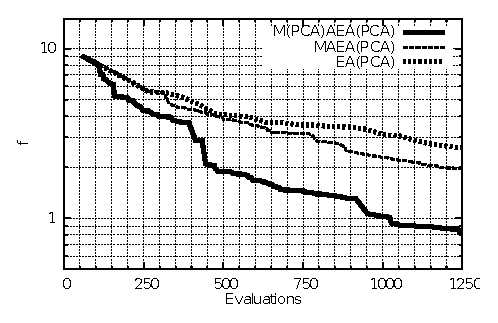
\includegraphics{1000_30d_pca_ipe.eps}}
\end{minipage}
\begin{minipage}[b]{0.5\linewidth}
 \centering
 \resizebox*{7.5cm}{!}{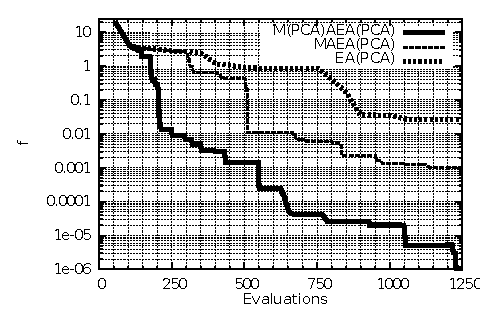
\includegraphics{30d_pca_ipe.eps}}
\end{minipage}
\caption{Μέσες καμπύλες σύγκλισης παραλλαγών των ΕΑ ή ΜΑΕΑ, που χρησιμοποιούν ΑσΚΣ, για το 30Δ ελλειψοειδές με  αριθμό κατάστασης $a=1000$ (αριστερά), και για την 30Δ συνάρτηση της σχέσης \ref{mm} (δεξιά).} 
\label{ellipse_t2_pca_ipe}
\end{figure} 
\pagebreak
Οι πορείες σύγκλισης των ΕΑ(\english{PCA}),    ΜΑΕΑ(\english{PCA}) και \linebreak Μ(\english{PCA})ΑΕΑ(\english{PCA}) για τα δύο αυτά προβλήματα παρουσιάζονται στο σχήμα \ref{ellipse_t2_pca_ipe}. Εκφράζουν και πάλι $10$ τρεξίματα βελτιστοποίησης με διαφορετική αρχικοποίηση της γεννήτριας τυχαίων αριθμών.  Παρατηρείται ότι η επιπρόσθετη χρήση υποβοηθούμενων απο ΑσΚΣ μεταπροτύπων επιφέρει επιπλέον μείωση του υπολογιστικού κόστους και στις δύο περιπτώσεις.


\section{Εφαρμογή: Σχεδιασμός 2Δ Πτερύγωσης Συμπιεστή}
Οι προτεινόμενες σε αυτό το κεφάλαιο μέθοδοι πιστοποιούνται, επίσης, στο σχεδιασμό-βελτιστοποίηση της αεροτομής μιας 2Δ πτερύγωσης συμπιεστή. Η πτερύγωση λειτουργεί σε $M_1=0.54$, $a_1=44^o$ και $Re=4\!\times\!10^5$ και στόχος είναι η ελαχιστοποίηση του συντελεστή των απωλειών ολικής πίεσης ($\omega$), σχέση \ref{omegaLosses}, υπό τους περιορισμούς ελάχιστου πάχους και ελάχιστης στροφής της ροής της ενότητας \ref{Drela1}. Χρησιμοποιείται το ίδιο λογισμικό αξιολόγησης. Η παραμετροποίηση της αεροτομής ορίζει συνολικά $27$ μεταβλητές σχεδιασμού.  

Πραγματοποιήθηκαν δύο διαδικασίες βελτιστοποίησης, η πρώτη με τον προϋπάρχοντα ΜΑΕΑ και η δεύτερη κάνοντας συνδυασμένη χρήση των δύο μεθόδων που προτάθηκαν σε αυτό το κεφάλαιο, δηλαδή τη μέθοδο Μ(\english{PCA})ΑΕΑ(\english{PCA}). 
   
Οι πορείες σύγκλισης για τις δύο αυτές διαδικασίες παρουσιάζονται στο σχήμα \ref{PCADrelaRes}, όπου είναι εμφανές το κέρδος που προκύπτει λόγω τόσο της ταχύτερης έναρξης της διαδικασίας ΠΠΑ όσο και της αποδοτικότερης εξέλιξης λόγω των προσαρμοσμένων τελεστών εξέλιξης. Περισσότερες πληροφορίες για τη ρύθμιση των παραμέτρων υπάρχουν στο πλήρες κείμενο της διατριβής.   
  

Η βέλτιστη αεροτομή, όπως αυτή προέκυψε από το συνδυασμό των προτεινόμενων μεθόδων παρουσιάζεται στο σχήμα \ref{PCADrelaRes2} και έχει απώλειες $\omega\!=\!0.01803$ και στροφή της ροής $\Delta a\!=\!30^o$ ενώ, παράλληλα, ικανοποιεί και όλους τους γεωμετρικούς περιορισμούς.  

\begin{figure}[h!]
\begin{minipage}[b]{1\linewidth}
 \centering
 \resizebox*{11cm}{!}{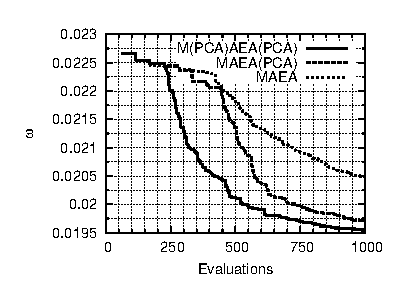
\includegraphics{CompConv_1.eps}}
\end{minipage}
\caption{Σχεδιασμός 2Δ πτερύγωσης συμπιεστή: Μέσες πορείες σύγκλισης από $10$ τρεξίματα των ΜΑΕΑ, ΜΑΕΑ(\english{PCA}) και  Μ(\english{PCA})ΑΕΑ(\english{PCA}). Ως κριτήριο τερματισμού τέθηκαν οι $1000$ κλήσεις του λογισμικού ΥΡΔ.} 
\label{PCADrelaRes}
\end{figure}


\begin{figure}[h!]
\begin{minipage}[b]{1\linewidth}
 \centering
 \resizebox*{14cm}{!}{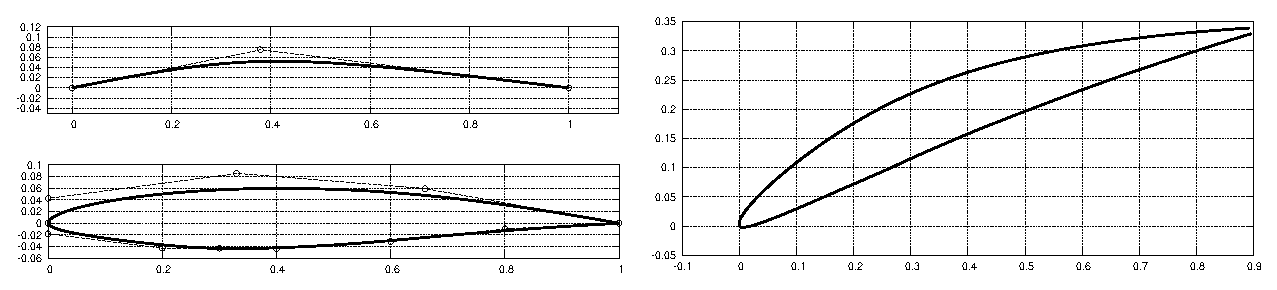
\includegraphics{ResD.eps}}
\end{minipage}
\caption{Σχεδιασμός 2Δ πτερύγωσης συμπιεστή: Η βέλτιστη αεροτομή, η οποία σχεδιάστηκε από το Μ(\english{PCA})ΑΕΑ(\english{PCA}). Αριστερά: Η μέση γραμμή και οι κατανομές πάχους για τις πλευρές υπερπίεσης και υποπίεσης, μαζί με τα πολύγωνα ελέγχου των πολυωνύμων \english{NURBS} που τις παρήγαγαν. Δεξιά: Η βέλτιστη αεροτομή, τοποθετημένη στην επιθυμητή γωνία κλίσης της πτερύγωσης. Η αεροτομή ικανοποιεί όλους τους τεθέντες περιορισμούς.} 
\label{PCADrelaRes2}
\end{figure}

%\begin{figure}[h!]
%\begin{minipage}[b]{1\linewidth}
% \centering
% \resizebox*{12cm}{!}{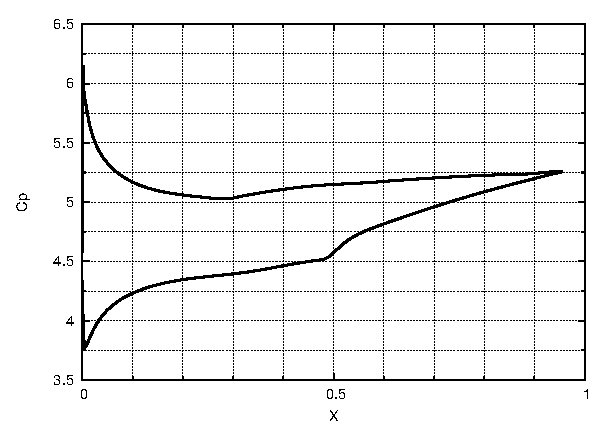
\includegraphics{Best_CP_PCA.eps}}
%\end{minipage}
%\caption{Σχεδιασμός 2Δ πτέρυγωσης συμπιεστή: Συντελεστής πίεσης $C_p$ για την βέλτιστη αεροτομή της εικόνας \ref{PCADrelaRes2}.} 
%\label{PCADrelaRes_cp}
%\end{figure}

% ---------------------------------------------------------------------------
% ----------------------- end of thesis sub-document ------------------------
% ---------------------------------------------------------------------------					% PCA
% change according to folder and file names
\ifpdf
    \graphicspath{{5/figures/PNG/}{5/figures/PDF/}{4/figures/}}
\else
    \graphicspath{{5/figures/EPS/}{5/figures/}}
\fi

%: ----------------------- contents from here ------------------------
\chapter{Βελτιστοποίηση Υδροδυναμικών Στροβιλομηχανών}  % top level followed by section, subsection
Σκοπός αυτού του κεφαλαίου είναι να παρουσιάσει το κέρδος, σε μείωση υπολογιστικού κόστους, που επιτεύχθηκε από τη χρήση των προτεινόμενων σε αυτήν τη διατριβή μεθόδων σε προβλήματα βιομηχανικής κλίμακας και, ειδικότερα, στο σχεδιασμό υδροδυναμικών στροβιλομηχανών. Αναλυτικά θα παρουσιασθούν α) η χρήση \english{KBD} κατά το σχεδιασμό-βελτιστοποίηση ενός υδροστροβίλου τύπου \english{Francis} και β) η χρήση  εξελικτικών τελεστών υποβοηθούμενων από ΑσΚΣ, δηλαδή της μεθόδου που συμβολίζεται με ΜΑΕΑ\english{(PCA)} κατά το σχεδιασμό-βελτιστοποίηση ενός υδροστροβίλου τύπου \english{Hydromatrix\circledR}. 

Η διαδικασία παραμετροποίησης και αξιολόγησης των υποψηφίων λύσεων (μέσω της αριθμητικής επίλυσης των εξισώσεων \english{Euler}) είναι όμοια και για τους δύο τύπους στροβιλομηχανών και παρουσιάζεται με λεπτομέρεια στο πλήρες κείμενο της διατριβής.   

Όπως θα φανεί στη συνέχεια, είναι επιθυμητό η βελτιστοποίηση  να επιδιώξει την ελαχιστοποίηση αρκετών διαφορετικών συναρτήσεων που εκφράζουν την ποιότητα των σχεδιαζόμενων στροβιλομηχανών ή των συνιστωσών τους και, μάλιστα, σε περισσότερα του ενός σημεία λειτουργίας. Παρότι υπάρχει η δυνατότητα το χρησιμοποιούμενο λογισμικό βελτιστοποίησης (ΕΑ ή ΜΑΕΑ) να αναζητήσει μέτωπα \english{Pareto} στον πολυδιάστατο χώρο, εν τούτοις, για πρακτικούς λόγους θα χρησιμοποιηθούν ως συναρτήσεις κόστους κατάλληλοι συγκερασμοί των προαναφερθεισών ποσοτήτων στα διάφορα σημεία λειτουργίας. Έτσι, οι ποσότητες που μετρούν ποιότητα, ως προς διάφορα χαρακτηριστικά, θα αναφέρονται ως «μετρικές ποιότητας» (\english{quality metrics}) και δεσμεύεται η χρήση του όρου «συνάρτηση κόστους» για τις συναρτήσεις που ελαχιστοποιούνται από τον ΕΑ ή τον ΜΑΕΑ ή κάθε παραλλαγή τους.   
Οι τέσσερις μετρικές ποιότητας που χρησιμοποιούνται για να ποσοτικοποιήσουν την ποιότητα κάθε υποψήφιας λύσης είναι: 
\begin{itemize}
\item{\textbf{$\sigma$:}} Μετρική σπηλαίωσης η οποία εκφράζει την «απόσταση» από την κατάσταση εμφάνισης του φαινομένου της σπηλαίωσης. 
\item{\textbf{M$_1$:}} Μετρική καλής συνεργασίας με τον αγωγό απαγωγής, η οποία εκφράζει την απόκλιση της κατανομής της περιφερειακής $C_u$ και μεσημβρινής $C_m$ συνιστώσας της ταχύτητας στην είσοδο του αγωγού απαγωγής από κατανομές-στόχους που θέτει ο σχεδιαστής. Επιδιώκεται, προφανώς, η ελαχιστοποίηση των παραπάνω αποκλίσεων.
\item{\textbf{M$_2$:}} Μετρική ομοιόμορφης φόρτισης του πτερυγίου, μέσω της οποίας επιδιώκεται η, κατά το δυνατό, ομοιομορφία της φόρτισης του πτερυγίου κατά την κατεύθυνση της χορδής.
\item{\textbf{M$_3$:}} Μετρική επιφάνειας άντλησης. Στην περίπτωση μη-ρυθμιζόμενων υδροδυναμικών μηχανών, όπως ο \english{Hydromatrix\circledR}, δημιουργούνται περιοχές του πτερυγίου της κινητής πτερύγωσης όπου η πλευρά υπερπίεσης έχει χαμηλότερη πίεση  από την πλευρά υποπίεσης. Το φαινόμενο εμφανίζεται συνήθως κατά τη λειτουργία σε μερικό φορτίο και είναι επιθυμητό  η έκταση του να ελαχιστοποιηθεί.   
\end{itemize}

\section{Βελτιστοποίηση Υδροστροβίλου $Francis$}
Η ενότητα αυτή αναφέρεται στο σχεδιασμό-βελτιστοποίηση του δρομέα ενός υδροστροβίλου $Francis$, κάνοντας χρήση της τεχνικής \english{KBD}. Ο σχεδιασμός συμπεριλαμβάνει, για λόγους στιβαρότητας κατά τη λειτουργία, τρία σημεία λειτουργίας: τα σημεία  μερικού (ΜΦ) και πλήρους φορτίου (ΠΦ) και το σημείο μέγιστης απόδοσης (ΜΑ). Στο πρόβλημα εμπλέκονται δύο συναρτήσεις-στόχοι ανά σημείο λειτουργίας, οριζόμενες μέσω των μετρικών $M_1$ και $M_2$, ως εξής 

\begin{eqnarray}
   f_1^i=M_1^i ~~~\&~~~ f_2^i=M_2^i 
   \label{ObjFrancis} 
\end{eqnarray}
όπου ο άνω δείκτης $i=1,2,3$ χαρακτηρίζει το σημείο λειτουργίας.

Οι προαναφερθέντες $2\times3=6$ συναρτήσεις-στόχοι ομαδοποιούνται σε $2$ συναρτήσεις κόστους με τη σχέση    

\begin{eqnarray}
   f_1=\sum^3_{i=1}w_if_1^i ~~~\&~~~ f_2=\sum^3_{i=1}w_if_2^i 
   \label{ObjFrancis2} 
\end{eqnarray}
όπου $w_i$ καθοριζόμενος συντελεστής βάρους ανά σημείο λειτουργίας (πίνακας \ref{op-weights}).

\begin{table}[h!]
\begin{center}
\begin{tabular}{ |c|l| }
\hline
Σημείο Λειτουργίας & Βάρος $(w_i)$\\
\hline
Μέγιστης Απόδοσης (ΜΑ), $i=1$ & 1.0\\
\hline
Μερικού Φορτίου  (ΜΦ), $i=2$ & 0.3\\
\hline
Πλήρους Φορτίου (ΠΦ), $i=3$ & 0.3\\
\hline
\end{tabular}
\caption{Βελτιστοποίηση υδροστροβίλου $Francis$: Συντελεστές Βαρύτητας ανά σημείο λειτουργίας.}
\label{op-weights}
\end{center}
\end{table}

 Ο υδροστρόβιλος $Francis$ έχει ρυθμιζόμενα οδηγά περύγια άρα η μετρική της επιφάνειας άντλησης ($Μ_3$) δεν χρειάζεται να χρησιμοποιηθεί. Έτσι όπως διατυπώθηκε το πρόβλημα, η μετρική που αφορά στη σπηλαίωση (σ) αλλά και το επιθυμητό υδραυλικό ύψος (Η) χρησιμοποιήθηκαν ως περιορισμοί (πίνακας \ref{Cons}).


\begin{table}[h!]
\begin{center}
\begin{tabular}{ |c|c|c| }
\hline
Σημείο Λειτουργίας  & $\sigma_i^{Hist}<\sigma$ & Υδραυλικό ύψος\\
\hline
ΜΑ & $\sigma_i^{Hist}<0.2$ & $|\Delta H|<1.5\%$\\
\hline
ΜΦ       & $\sigma_i^{Hist}<0.2$ & $|\Delta H|<5\%$\\
\hline
ΠΦ       & $\sigma_i^{Hist}<0.2$ & $|\Delta H|<5\%$\\
\hline
\end{tabular}
\caption{Βελτιστοποίηση υδροστροβίλου $Francis$: Τεθέντες περιορισμοί, σχετικοί με τη σπηλαίωση (στη μορφή της μετρικής σ, ορισμός του $\sigma_i^{Hist}$ υπάρχει στο πλήρες κείμενο της διατριβής) και το υδραυλικό ύψος Η, στα τρία σημεία λειτουργίας. Η ποσότητα $|\Delta H|$ εκφράζει την απόλυτη τιμή της διαφοράς του ύψους Η από την επιθυμητή τιμή αυτού στο κάθε σημείο λειτουργίας. Με τις χρησιμοποιούμενες οριακές συνθήκες, η ανάλυση της ροής στο δρομέα με λογισμικό ΥΡΔ έχει ως εξαγόμενο το υδραυλικό ύψος Η το οποίο, σε κάθε σημείο λειτουργίας, οφείλει να έχει δεδομένη τιμή, με επιθυμητή ανοχή $|\Delta H|$.}
\label{Cons}
\end{center}
\end{table}


Η γεωμετρία του προς βελτιστοποίηση δρομέα παραμετροποιείται με $336$ μεταβλητές σχεδιασμού, όπως αυτές παρουσιάζονται στο αντίστοιχο κεφάλαιο του πλήρους κειμένου της διατριβής. 


\subsection{Αρχειοθετημένοι Σχεδιασμοί Βάσης}
Για την υποστήριξη της διαδικασίας σχεδιασμού-βελτιστοποίησης με τη μέθοδο $KBD$, εντοπίστηκαν τρεις ($m\!=\!3$) αρχειοθετημένοι σχεδιασμοί, οι οποίοι σχεδιάστηκαν στο παρελθόν για «κοντινά», σε σχέση με το επιθυμητό, σημεία λειτουργίας. Αυτοί οι σχεδιασμοί χρησιμοποιούνται  ως σχεδιασμοί βάσης κατά την εφαρμογή της μεθόδου \english{KBD}. Οι επιδόσεις των σχεδιασμών βάσης στα επιθυμητά σημεία λειτουργίας παρουσιάζονται στον πίνακα \ref{reuse}.

\begin{table}[h!]
\begin{center}
\begin{tabular}{ |c|c|c|c|c|c| }
\hline
Σχεδιασμός & ΣΛ & $M_1$ & $M_2$  & $\sigma_i^{Hist}$ & $|\Delta H|$\\
Βάσης & & & & &\\
\hline
Β1 & ΜΑ & $0.472$ & $0.538$ & $0.21 >0.2$ * & $ 5\% >1.5\%$ * \\
Β1 & ΜΦ & $0.552$ & $0.824$ & $0.23 > 0.2$ * & $ 3.6\% <5\%$ \\
Β1 & ΠΦ & $0.408$ & $0.594$ & $0.2 = 0.2$  & $ 5.7\% >5\%$ * \\
\hline
\hline
Β2 & ΜΑ & $0.563$ & $0.922$ & $0.22 > 0.2$ * & $ 3.8\% >1.5\%$ * \\
Β2 & ΜΦ & $0.534$ & $0.888$ & $0.24 > 0.2$ * & $ 2.6\% <5\%$  \\
Β2 & ΠΦ & $0.522$ & $1.178$ & $0.22 > 0.2$ * & $ 4.8\% <5\%$  \\
\hline
\hline
Β3 & ΜΑ & $0.402$ & $0.663$ & $0.19 < 0.2$  & $ 6.8\% >1.5\%$ * \\
Β3 & ΜΦ & $0.515$ & $0.808$ & $0.21 > 0.2$ * & $ 6.9\% >5\%$ * \\
Β3 & ΠΦ & $0.257$ & $0.896$ & $0.18 < 0.2$  & $ 7.1\% >5\%$ * \\
\hline
\end{tabular}
\caption{Βελτιστοποίηση Υδροστροβίλου $Francis$: Οι μετρικές ποιότητας ($M_1$ και $M_2$) που σχηματίζουν τους στόχους και οι περιορισμοί (σ και $|\Delta H|$) για τους σχεδιασμούς βάσης ($B1, B2$ και $B3$) για τα επιθυμητά σημεία λειτουργίας. Ο αστερίσκος (*) στους περιορισμούς υποδηλώνει ότι ο υπόψη σχεδιασμός βάσης παραβιάζει τον αντίστοιχο περιορισμό.}
\label{reuse}
\end{center}
\end{table}

\begin{figure}[h!]
\begin{minipage}[b]{0.5\linewidth}
 \centering
 \resizebox*{6.5cm}{!}{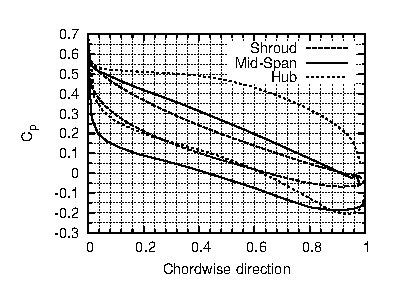
\includegraphics{Load_B1.eps}}
\end{minipage}
\begin{minipage}[b]{0.5\linewidth}
 \centering
 \resizebox*{6.5cm}{!}{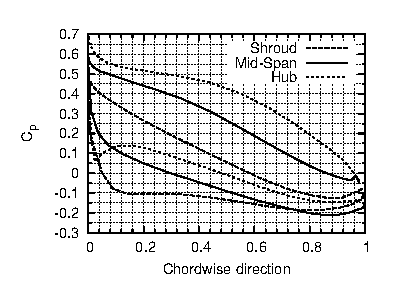
\includegraphics{Load_B2.eps}}
\end{minipage}
\begin{minipage}[b]{1\linewidth}
 \centering
 \resizebox*{6.5cm}{!}{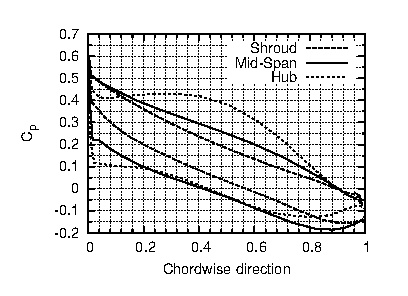
\includegraphics{Load_B3.eps}}
\end{minipage}
\caption{Βελτιστοποίηση υδροστροβίλου $Francis$: Κατανομές του συντελεστή πίεσης $C_p$ κατά μήκος της χορδής για τρεις χαρακτηριστικές καθ' ύψος  θέσεις στο πλήμνη , \english{(hub)}, μέσο ύψος \english{(mid-span)} και στεφάνη \english{(shroud)}  για τους σχεδιασμούς βάσης, Β1 (πάνω-αριστερά), Β2 (πάνω-δεξιά) και Β3 (κάτω).}
\label{Francis-LOAD}
\end{figure}


Η ποιότητα των σχεδιασμών βάσης, όταν αυτοί χρησιμοποιηθούν στα επιθυμητά σημεία, είναι αρκετά κακή όπως φαίνεται στον πίνακα \ref{reuse}. Αυτό γίνεται ακόμη πιο εμφανές από τα σχήματα \ref{Francis-LOAD}, όπου φαίνεται η ανομοιομορφία φόρτισης των πτερυγίων του δρομέα, και \ref{Francis-OUT}, όπου φαίνεται η μεγάλη απόκλιση από τις κατανομές-στόχους της περιφερειακής και μεσημβρινής ταχύτητας στην έξοδο, άρα και η κακή συνεργασία που θα είχαν με τον αγωγό απαγωγής.         


\begin{figure}[h!]
\begin{minipage}[b]{0.5\linewidth}
 \centering
 \resizebox*{6cm}{!}{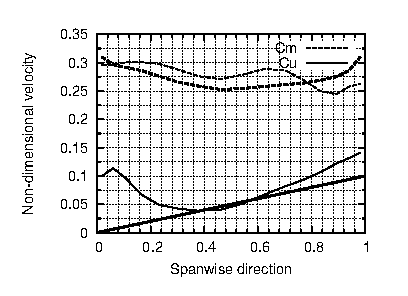
\includegraphics{OUTLET_B1.eps}}
\end{minipage}
\begin{minipage}[b]{0.5\linewidth}
 \centering
 \resizebox*{6cm}{!}{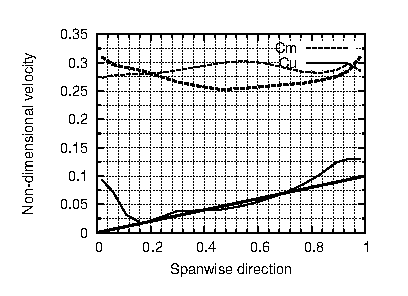
\includegraphics{OUTLET_B2.eps}}
\end{minipage}
\begin{minipage}[b]{1\linewidth}
 \centering
 \resizebox*{6cm}{!}{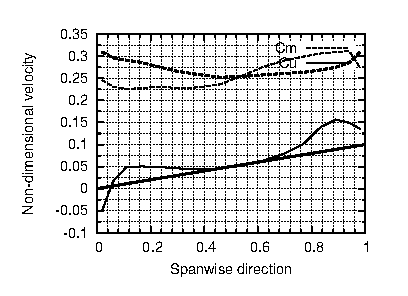
\includegraphics{OUTLET_B3.eps}}
\end{minipage}
\caption{Βελτιστοποίηση υδροστροβίλου $Francis$: Κατανομές περιφερειακής ($C_u$) και μεσημβρινής ($C_m$)  συνιστώσας της ταχύτητας εξόδου για τους σχεδιασμούς βάσης, Β1 (πάνω-αριστερά), Β2 (πάνω-δεξιά) και Β3 (κάτω) σε αντιπαραβολή με τις αντίστοιχες κατανομές-στόχους που καθορίστηκαν από το σχεδιαστή.}
\label{Francis-OUT}
\end{figure}

Κατά την εφαρμογή της μεθόδου $KBD$, οι μεταβλητές σχεδιασμού ομαδοποι-ούνται σε $6$ ομάδες και, μαζί με τη μεταβλητή  προεκβολής
$\Psi$, δημιουργούν τις $19$ ($=3\times6+1$) μεταβλητές βελτιστοποίησης. Η λεπτομερής ομαδοποίηση περιγράφεται στο πλήρες κείμενο της διατριβής. Είναι, εκ των πραγμάτων, συγκριτικά πλεονεκτικότερη η χρήση ΕΑ (ή ΜΑΕΑ) για την αναζήτηση του βέλτιστου συνόλου των $19$, αντί των $336$ (της κανονικής παραμετροποίησης), μεταβλητών.   

\subsection{Αποτελέσματα - Συγκρίσεις}
Ο σχεδιασμός πραγματοποιήθηκε κάνοντας χρήση ενός ΕΑ και ενός ΜΑΕΑ(\english{KBD}). Ο ρυθμός σύγκλισης των συναρτήσεων κόστους, σε κάθε περίπτωση παρουσιάζεται στο σχήμα \ref{Francis-Res}, όπου σχεδιάζεται ο δείκτης υπερόγκου (\english{hypervolume indicator}, \cite{Zitz2007}). Στο συμβατικό ΕΑ ήταν ιδιαίτερα αναποτελεσματική η χρήση μεταπροτύπων με αποδοτικό τρόπο λόγω του μεγάλου αριθμού μεταβλητών σχεδιασμού ($336$), όπως άλλωστε παρατηρήθηκε και κατά την εφαρμογή της ενότητας \ref{Drela1}. Αντίθετα, κάνοντας χρήση της μεθόδου \english{KBD} γίνεται ξανά δυνατή η χρήση μεταπροτύπων μέσω της τεχνικής ΠΠΑ, η οποία ξεκινά όταν στη βάση δεδομένων του ΜΑΕΑ αποθηκευθούν $150$ (μη-τιμωρημένα με «ποινή θανάτου») άτομα. Η ρύθμιση των παραμέτρων των δύο ΕΑ παρουσιάζεται στο πλήρες κείμενο της διατριβής. Και στις δύο διαδικασίες βελτιστοποίησης, οι 3 σχεδιασμοί βάσης επιβάλλονται ως μέλη του πληθυσμό της πρώτης γενιάς του ΕΑ.      
          
\begin{figure}[h!]
\begin{minipage}[b]{0.5\linewidth}
 \centering
 \resizebox*{7.0cm}{!}{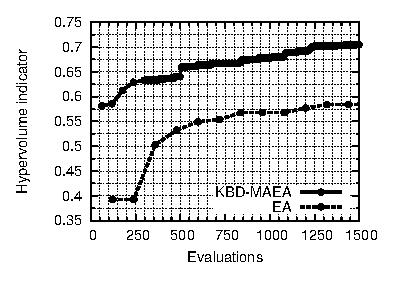
\includegraphics{HypComp.eps}}
\end{minipage}
\begin{minipage}[b]{0.5\linewidth}
 \centering
 \resizebox*{7.0cm}{!}{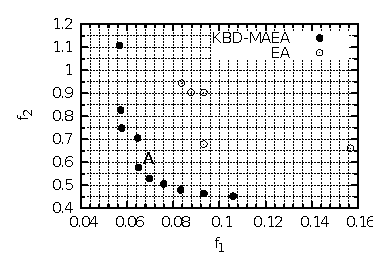
\includegraphics{Comp.eps}}
\end{minipage}
\caption{Βελτιστοποίηση υδροστροβίλου $Francis$:  Σύγκριση πορείας του δείκτη υπερόγκου για τη δικριτηριακή βελτιστοποίηση με ΕΑ και ΜΑΕΑ(\english{KBD}) (αριστερά). Μέτωπα μη-κυριαρχούμενων λύσεων (για Μ=$2$) για τους ΕΑ και ΜΑΕΑ(\english{KBD}) που υπολογίστηκαν έχοντας ως κριτήριο τερματισμού τις $1500$ αξιολογήσεις με το λογισμικό ΥΡΔ (δεξιά).}
\label{Francis-Res}
\end{figure}

Είναι εμφανές (σχήμα \ref{Francis-Res}, αριστερά) ότι η προτεινόμενη μέθοδος, ΜΑΕΑ(\english{KBD}): α) εκκινεί από υψηλότερη τιμή του δείκτη υπερόγκου κάτι που υποδηλώνει ότι ο τρόπος  καθορισμού σημαντικότητας στις περιοχές του χώρου σχεδιασμού είναι πολύ κοντά στη φυσική του προβλήματος και β) συνεχίζει με συνεχώς καλύτερες τιμές για όλη τη διάρκεια της βελτιστοποίησης. Η ανωτερότητα της μεθόδου \english{KBD} γίνεται ακόμη περισσότερο εμφανής παρατηρώντας τα τελικά μέτωπα των μη-κυριαρχούμενων λύσεων τα οποία αντιστοιχούν στο ίδιο υπολογιστικό κόστος ($1500$ αξιολογήσεις) (σχήμα \ref{Francis-Res}, δεξιά). Τέλος, από το μέτωπο των μη-κυριαρχούμενων λύσεων που προέκυψε από το       ΜΑΕΑ(\english{KBD}), επιλέγεται το άτομο Α το οποίο και αναλύεται περαιτέρω στη συνέχεια (σχήμα \ref{design-bases-a}).


\begin{figure}[h!]
\begin{minipage}[b]{1\linewidth}
 \centering
 \resizebox*{10.0cm}{!}{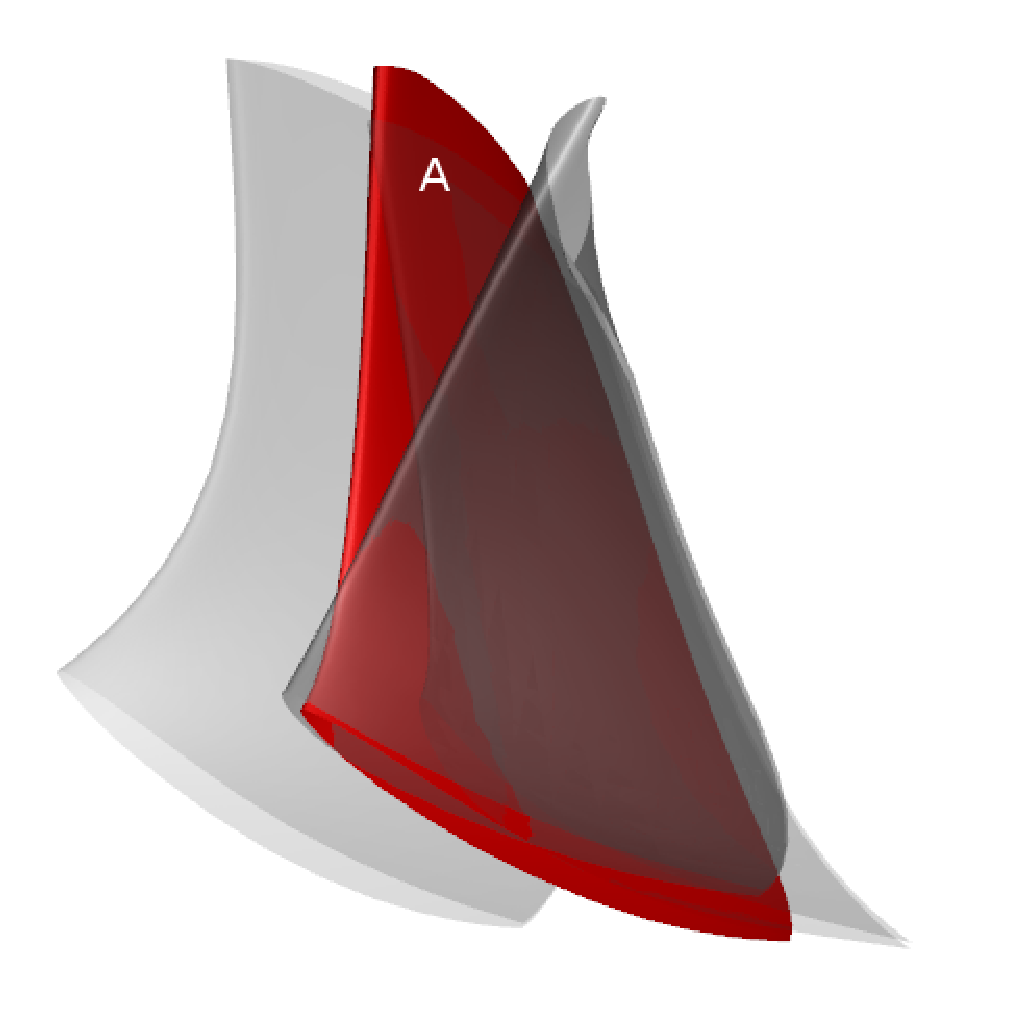
\includegraphics{final.eps}}
\end{minipage}
\caption{Βελτιστοποίηση υδροστροβίλου $Francis$: Το πτερύγιο του δρομέα του επιλεγμένου σχεδιασμού Α και οι τρεις σχεδιασμοί βάσης που χρησιμοποιήθηκαν.}
\label{design-bases-a}
\end{figure}

\begin{table}[h!]
\begin{center}
\begin{tabular}{ |c|c|c|c|c|c| }
\hline
Σχεδιασμός & ΣΛ & $M_1$ & $M_2$  &  $\sigma_i^{Hist}$ & $|\Delta H|$\\
\hline
A & ΜΑ & $0.001$ & $0.302$ & $0.18 < 0.2$ & $ 1.1\% <1.5\%$ \\
A & ΜΦ & $0.086$ & $0.409$ & $0.19 < 0.2$ & $ 1.5\% <5\%$ \\
A & ΠΦ & $0.092$ & $0.504$ & $0.18 < 0.2$ & $ 4.1\% <5\%$  \\
\hline
\end{tabular}
\caption{Βελτιστοποίηση υδροστροβίλου $Francis$: Οι μετρικές ποιότητας ($M_1$ και $M_2$) που σχηματίζουν τους στόχους και οι περιορισμοί (σ και $|\Delta H|$) για το σχεδιασμό Α για τα τρία  υπόψη σημεία λειτουργίας (ΜΑ, ΜΦ και ΠΦ). Ο σχεδιασμός Α ικανοποιεί όλους τους περιορισμούς.}
\label{Asum}
\end{center}
\end{table}

Οι κατανομές του συντελεστή πίεσης $C_p$ σχεδιασμένες στις επιφάνειες του δρομέα του σχεδιασμού Α, στα τρία σημεία λειτουργίας, παρουσιάζονται στο σχήμα \ref{Francis-A}. Επιπλέον, για το σημείο ΜΑ, παρουσιάζονται και αναλυτικά οι κατανομές $C_p$ (σχήμα \ref{Francis-A-cp}, αριστερά) σχεδιασμένες στο πλήμνη , \english{(hub)}, στο μέσο ύψος \english{(mid-span)} και στην στεφάνη \english{(shroud)} της πτερύγωσης. Είναι εμφανής η ποιότητα του σχεδιασμού τόσο όσον αφορά στην ισοκατανεμημένη φόρτιση όσο και στην ασφάλεια από σπηλαίωση. Ακόμη, παρουσιάζονται κατανομές $C_u$ και $C_m$ στην έξοδο (σχήμα \ref{Francis-A-cp}, δεξιά) μαζί με τις κατανομές-στόχους.

\begin{figure}[h!]
\begin{minipage}[b]{0.5\linewidth}
 \centering
 \resizebox*{6cm}{!}{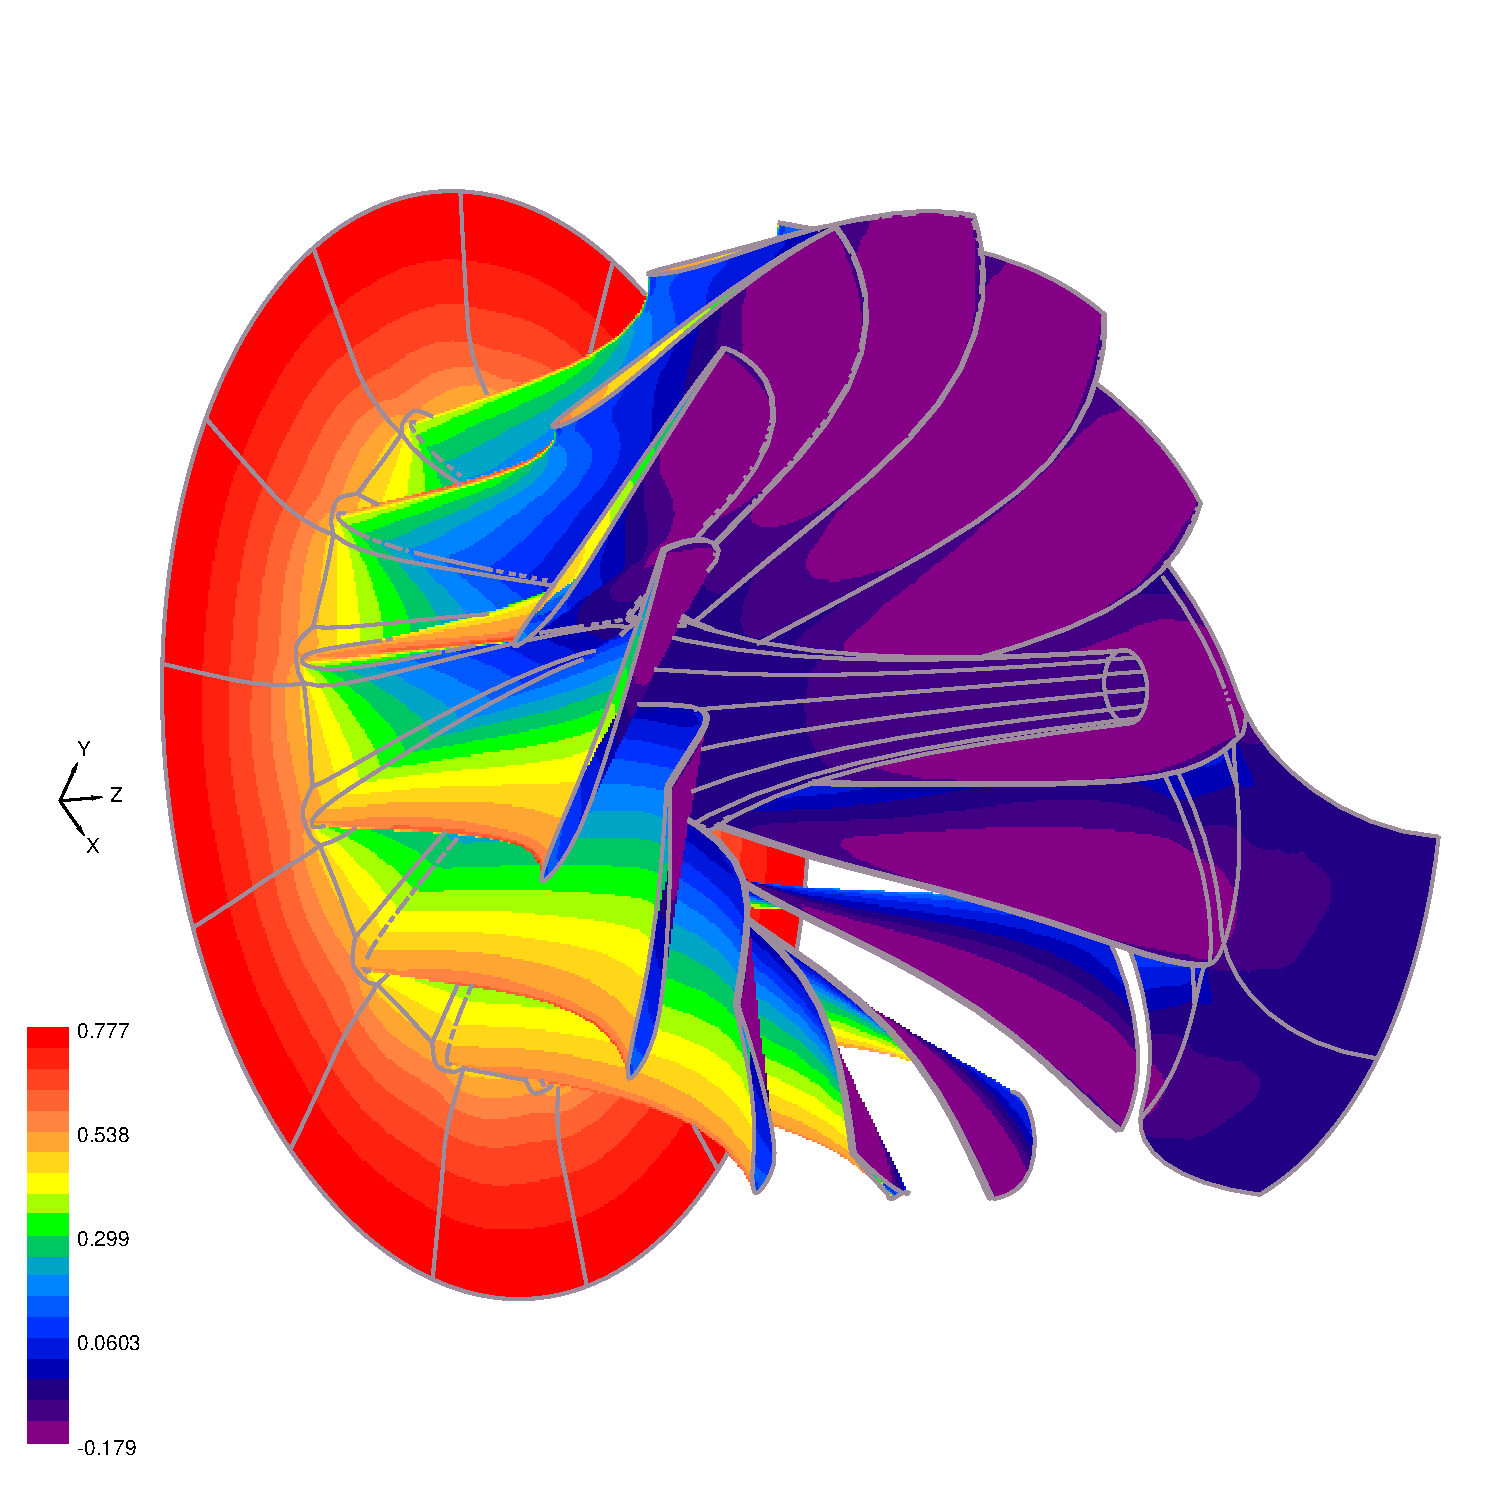
\includegraphics{ABE.eps}}
\end{minipage}
\begin{minipage}[b]{0.5\linewidth}
 \centering
 \resizebox*{6cm}{!}{\includegraphics{APL.eps}}
\end{minipage}
\begin{minipage}[b]{1\linewidth}
 \centering
 \resizebox*{6cm}{!}{\includegraphics{AFL.eps}}
\end{minipage}
\caption{Βελτιστοποίηση υδροστροβίλου $Francis$: Κατανομές $C_p$ στο δρομέα του σχεδιασμού Α στα τρία σημεία λειτουργίας: ΜΑ (πάνω-αριστερά), ΜΦ (πάνω-δεξιά) και ΠΦ (κάτω).}
\label{Francis-A}
\end{figure}


\begin{figure}[h!]
\begin{minipage}[b]{0.5\linewidth}
 \centering
 \resizebox*{6.5cm}{!}{\includegraphics{Load_A.eps}}
\end{minipage}
\begin{minipage}[b]{0.5\linewidth}
 \centering
 \resizebox*{6cm}{!}{\includegraphics{OUTLET_A.eps}}
\end{minipage}
\caption{Βελτιστοποίηση υδροστροβίλου $Francis$:  Κατανομές $C_p$ για το δρομέα του σχεδιασμού Α στο σημείο ΜΑ (αριστερά). Κατανομές των συνιστωσών της ταχύτητας εξόδου $C_u$ και $C_m$ για το σχεδιασμό Α στο σημείο ΜΑ (δεξιά).}
\label{Francis-A-cp}
\end{figure}

\FloatBarrier

\section{Βελτιστοποίηση Υδροστροβίλου $Hydromatrix\circledR$}

Η ενότητα αυτή παρουσιάζει το σχεδιασμό-βελτιστοποίηση ενός υδροστροβίλου $Hydromatrix\circledR$ κάνοντας χρήση ΕΑ με τους υποβοηθούμενους από ΑσΚΣ εξελικτικούς τελεστές, δηλαδή της μεθόδου που αναφέρεται ως ΜΑΕΑ(\english{PCA}). Ο σχεδιασμός γίνεται σε τρία σημεία λειτουργίας: το σημείο μέγιστης απόδοσης (ΜΑ) και τα σημεία πλήρους (ΠΦ) και μερικού (ΜΦ) φορτίου. Ο συνδυασμός των μετρικών ποιότητας σε δύο  στόχους ανά σημείο λειτουργίας γίνεται με άθροισμα μέσω συντελεστών βαρύτητας (πίνακας \ref{op-weights-M1}), ως


\begin{eqnarray}
   f_1^i=\alpha ^i  M_1^i ~~~,~~~ f_2^i=\beta ^i Μ_2^i+\gamma ^i  \sigma_i^{Hist} +\delta ^i  Μ_3^i 
   \label{ObjFrancis} 
\end{eqnarray}
όπου ο άνω δείκτης $i=1,2,3$ αναφέρεται στο σημείο λειτουργίας.


\begin{table}[h!]
\begin{center}
\begin{tabular}{ |l|r|r|r|c| }
%\hline
%\multicolumn{4}{|c|}{Βάρη} & F \\
\hline
& ΜΑ, $i\!=\!1$ & ΜΦ, $i\!=\!2$ & ΠΦ, $i\!=\!3$ &  Στόχος\\
\hline
α ($M_1$) & 1.0            &0.0            &0.0 & $f_1$\\
\hline
β ($M_2$) &0.2    &0.0            &0.0  & $f_2$\\
\hline
γ ($\sigma_i^{Hist}$) &1.0            &1.0            &1.0 & $f_2$\\
\hline
δ ($M_3$) &0.0            &100.0  &100.0 & $f_2$\\
\hline
\end{tabular}
\caption{Βελτιστοποίηση υδροστροβίλου $Hydromatrix\circledR$: Συντελεστές βαρύτητας κατά την ομαδοποίηση των μετρικών σε δύο στόχους ανά σημείο λειτουργίας.}
\label{op-weights-M1}
\end{center}
\end{table}

 Ο συνδυασμός των συναρτήσεων-στόχων $f^i_1$ και $f^i_2$ για όλα τα σημεία λειτουργίας σε δύο, τελικά, συναρτήσεις-κόστους (M=$2$) γίνεται μέσω των συντελεστών βαρύτητας $w_i$ του πίνακα \ref{op-weights-M2} ως

\begin{eqnarray}
   f_1=\sum^3_{i=1}w_if_1^i ~~~,~~~ f_2=\sum^3_{i=1}w_if_2^i 
   \label{ObjFrancis2} 
\end{eqnarray}

\begin{table}[h!]
\begin{center}
\begin{tabular}{ |c|l| }
\hline
Σημείο λειτουργίας & $w_i$\\
\hline
Μέγιστης Απόδοσης (ΜΑ), $i\!=\!1$  & 1.0\\
\hline
Μερικού Φορτίου  (ΜΦ), $i\!=\!2$ & 0.1\\
\hline
Πλήρους Φορτίου (ΠΦ), $i\!=\!3$  & 0.1\\
\hline
\end{tabular}
\caption{Βελτιστοποίηση υδροστροβίλου $Hydromatrix\circledR$: Συντελεστές βαρύτητας $w_i$ ανά σημείο λειτουργίας.}
\label{op-weights-M2}
\end{center}
\end{table}

Στο παρόν πρόβλημα βελτιστοποίησης η μετρική που αφορά στη σπηλαίωση αναβαθμίζεται από περιορισμό σε μια από τις συνιστώσες της $f_2$. Επίσης, ο περιορισμός που αφορά στη λειτουργία στο επιθυμητό σημείο λειτουργίας δεν υφίσταται για το σημείο ΜΑ αφού, για κάθε υποψήφια λύση, πραγματοποιείται μια δεύτερη εσωτερική διαδικασία βελτιστοποίησης η οποία ρυθμίζει τη γωνία μετάλλου στην έξοδο της σταθερής πτερύγωσης ούτως ώστε ο σχεδιασμός να λειτουργεί στο επιθυμητό σημείο. Παρόλα αυτά, παραμένει απαραίτητη η χρήση του σχετικού περιορισμού που αφορά στη λειτουργία στα υπόλοιπα δύο σημεία λειτουργίας. Συγκεκριμένα, ο περιορισμός αυτός αφορά στην επιθυμητή παροχή όγκου, επιτρέποντας ποσοστιαία απόκλιση  της παροχής όγκου ρευστού $|\Delta Q| < 5\%$, κατ' αντιστοιχία με τους περιορισμούς $|\Delta Η|$ της προηγούμενης ενότητας.  Σημειώνεται ότι η ανάλυση της ροής στο δρομέα με λογισμικό ΥΡΔ έχει, σύμφωνα με τις επιβαλλόμενες οριακές συνθήκες, ως δεδομένο το ύψος Η και ως εξαγόμενο την παροχή $Q$.
              

\subsection{Αποτελέσματα - Συγκρίσεις}
Ό σχεδιασμός πραγματοποιήθηκε κάνοντας χρήση ενός MAΕΑ και ενός ΜΑΕΑ(\english{PCA}). Οι πορείες σύγκλισης των δύο παρουσιάζονται στο σχήμα \ref{Matrix-Res} χρησιμοποιώντας το δείκτη υπερόγκου, \cite{Zitz2007}, ως κριτήριο σύγκρισης.  Η ακριβής ρύθμιση των παραμέτρων των δύο δικριτηριακών MAΕΑ που δοκιμάστηκαν παρουσιάζεται στο πλήρες κείμενο της διατριβής. 

\begin{figure}[h!]
\begin{minipage}[b]{0.5\linewidth}
 \centering
 \resizebox*{7.5cm}{!}{\includegraphics{nhyperv.eps}}
\end{minipage}
\begin{minipage}[b]{0.5\linewidth}
 \centering
 \resizebox*{7.0cm}{!}{\includegraphics{fparetos.eps}}
\end{minipage}
\caption{Βελτιστοποίηση  υδροστροβίλου $Hydromatrix\circledR$: Σύγκριση της πορείας του δείκτη υπερόγκου για τους δικριτηριακούς ΜΑΕΑ και ΜΑΕΑ(\english{PCA}) (αριστερά). Μέτωπα μη-κυριαρχούμενων λύσεων για τις δύο μεθόδους που δοκιμάστηκαν επιβάλλοντας τερματισμό τους στις $2000$ αξιολογήσεις με το λογισμικό ΥΡΔ (δεξιά).}
\label{Matrix-Res}
\end{figure}

Το κέρδος από τη χρήση των προτεινόμενων τελεστών εξέλιξης υποβοηθούμενων από την ΑσΚΣ παρουσιάζεται στο σχήμα \ref{Matrix-Res}. Επίσης, παρουσιάζονται τα μέτωπα των μη-κυριαρχούμενων λύσεων που υπολογίστηκαν από τις δύο μεθόδους για το ίδιο υπολογιστικό κόστος ($2000$ αξιολογήσεις με το λογισμικό ΥΡΔ). Τέλος, από τα μέλη του μετώπου \english{Pareto} επιλέγεται ο σχεδιασμός Α και αναλύεται λεπτομερώς.  

Η ποιότητα του σχεδιασμού Α, όσον αφορά στην ποιότητα της φόρτισης και στη συνεργασιμότητα με τον αγωγό απαγωγής, παρουσιάζεται στο σχήμα \ref{Matrix-A} όπου απεικονίζονται τόσο οι κατανομές $C_p$ για τα τρία σημεία λειτουργίας που ενδιαφέρουν όσο και οι κατανομές των ταχυτήτων εξόδου $C_u$ και $C_m$. Στο ίδιο σχήμα εμπεριέχεται και πληροφορία για τη σπηλαίωση (λαμβάνεται από την ελάχιστη τιμή του $C_p$ για κάθε σημείο λειτουργίας) όπως, επίσης, και για την επιφάνεια άντλησης (διασταυρούμενες κατανομές $C_p$ στο σημείο ΜΦ).      

\begin{figure}[h!]
\begin{minipage}[b]{0.5\linewidth}
 \centering
 \resizebox*{6.5cm}{!}{\includegraphics{LoadBE_M.eps}}
\end{minipage}
\begin{minipage}[b]{0.5\linewidth}
 \centering
 \resizebox*{6.5cm}{!}{\includegraphics{LoadPL_M.eps}}
\end{minipage}
\begin{minipage}[b]{0.5\linewidth}
 \centering
 \resizebox*{6.5cm}{!}{\includegraphics{LoadFL_M.eps}}
\end{minipage}
\begin{minipage}[b]{0.5\linewidth}
 \centering
 \resizebox*{6cm}{!}{\includegraphics{OUTLETMATRIX.eps}}
\end{minipage}
\caption{Βελτιστοποίηση  υδροστροβίλου $Hydromatrix\circledR$: Κατανομές συντελεστή πίεσης ($C_p$) κατά μήκος της χορδής για το σχεδιασμό Α στα τρία σημεία λειτουργίας, ΜΑ (πάνω-αριστερά), ΜΦ (πάνω-δεξιά) και ΠΦ (κάτω-αριστερά). Κατανομές $C_u$ και $C_m$ για το σημείο ΜΑ, στην έξοδο του δρομέα, μαζί με τις χρησιμοποιηθείσες κατανομές-στόχους (κάτω-δεξιά).}
\label{Matrix-A}
\end{figure}

Η εμφάνιση επιφάνειας άντλησης γίνεται καλύτερα αντιληπτή στο σχήμα \ref{Matrix-A-2}. Οι γραμμές ροής κοντά στο κέλυφος στεφάνης (\english{shroud}) του δρομέα για το σημείο ΜΦ υποδηλώνουν ότι η ροή «συναντά» το πτερύγιο του δρομέα στην πλευρά υποπίεσης δημιουργώντας έτσι μία περιοχή υψηλότερων πιέσεων από τις αντίστοιχες στην πλευρά υπερπίεσης. Αυτή η ανεπιθύμητη συμπεριφορά δεν μπορεί να αποφευχθεί ε-ντελώς λόγω της φύσης του συγκεκριμένου τύπου υδροστρόβιλου αλλά η διαδικασία βελτιστοποίησης επιτυγχάνει τον περιορισμό της.       

\begin{figure}[h!]
\begin{minipage}[b]{0.5\linewidth}
 \centering
 \resizebox*{7cm}{!}{\includegraphics{BE.eps}}
\end{minipage}
\begin{minipage}[b]{0.5\linewidth}
 \centering
 \resizebox*{7cm}{!}{\includegraphics{PartLoad.eps}}
\end{minipage}
\begin{minipage}[b]{1\linewidth}
 \centering
 \resizebox*{7cm}{!}{\includegraphics{FL.eps}}
\end{minipage}
\caption{Βελτιστοποίηση  υδροστροβίλου $Hydromatrix\circledR$: Ισοβαρείς επί της επιφάνειας του πτερυγίου και γραμμές ροής στην περιοχή του κελύφους στεφάνης (\english{shroud}) για το σχεδιασμό Α, μέλους του υπολογισθέντος μετώπου \english{Pareto}, στα τρία μελετούμενα σημεία λειτουργίας, ΜΑ (πάνω-αριστερά), ΜΦ (πάνω-δεξιά) και ΠΦ (κάτω).}
\label{Matrix-A-2}
\end{figure}


% ---------------------------------------------------------------------------
% ----------------------- end of thesis sub-document ------------------------
					% HYDRO
% this file is called up by thesis.tex
% change according to folder and file names
\ifpdf
    \graphicspath{{6/figures/PNG/}{6/figures/PDF/}{6/figures/}}
\else
    \graphicspath{{6/figures/EPS/}{6/figures/}}
\fi

%: ----------------------- contents from here ------------------------
% content in this file will be fed into the main document

\chapter{Βελτιστοποίηση Περιφερειακής Πτερύγωσης Συμπιεστή} % top level followed by section, % ---------------------------------------------------------------------------
Στόχος αυτού του κεφαλαίου είναι η βελτιστοποίηση της περιφερειακής πτερύγωσης συμπιεστή που βρίσκεται εγκατεστημένη στο ΕΘΣ/ΕΜΠ. Η πτερύγωση σχεδιάστηκε από τη \english{SNECMA} και έχει, στο παρελθόν, χρησιμοποιηθεί για τη μελέτη της ροής σε πτερυγώσεις με ακτινικό διάκενο (σχήμα \ref{res:ntua_blade:blade}) για υψηλούς αριθμούς \english{Mach} \footnote{\english{
European project «Advanced Civil Core Compressor Aerodynamics», AER2-CT92-0039, 1/1/1993-30/9/1996.}}. Παρουσίαση της διάταξης υπάρχει στο πλήρες κείμενο της διατριβής.  
   
\begin{figure}[h!]
\centering
  \includegraphics[width=.5\textwidth]{blade.eps}
  \caption{Βελτιστοποίηση περιφερειακής πτερύγωσης συμπιεστή: Τα πτερύγια στηρίζονται στο εξωτερικό κέλυφος (\english{shroud}) ενώ  το ακτινικό διάκενο δημιουργείται στην «επαφή» με το εσωτερικό κέλυφος (\english{hub}). Ο λόγος ακτίνων των δύο κελυφών είναι $R_{hub}/R_{shroud}=0.75$.}
  \label{res:ntua_blade:blade}
\end{figure}

Το πρόβλημα βελτιστοποίησης του σχήματος της (σταθερής κατά την ακτινική κατεύθυνση) αεροτομής του πτερυγίου αντιμετωπίζεται ως πρόβλημα μονοκριτηριακής βελτιστοποίησης  με περιορισμούς ελάχιστου πάχους σε τρεις θέσεις της αεροτομής, στο  $30\%$, $60\%$ και $90\%$ της χορδής. Το ελάχιστο αποδεκτό πάχος σε κάθε θέση καθορίζεται στο $90\%$ του αντίστοιχου πάχους του υπάρχοντος σχεδιασμού. Επιπλέον, επιβάλλεται περιορισμός ως προς τη μέση γωνία εξόδου ροής ($\alpha_2<53^o$). Η μελέτη έγινε για ακτινικό διάκενο ίσο με το $2\%$ του μήκους της χορδής.    

Η βελτιστοποίηση πραγματοποιήθηκε έχοντας ως μοναδική προς ελαχιστοποί-ηση συνάρτηση κόστους το μέσο συντελεστή απωλειών ολικής πίεσης $PLC_{av}$.  Η ποσότητα $PLC_{av}$ ορίζεται ως η μέση τιμή των τιμών του αντίστοιχου συντελεστή $PLC(r)$ σε κάθε ακτίνα ($r$) ανάμεσα στα δύο κελύφη. Η τελευταία δίνεται από τη σχέση 
\begin{equation}
PLC(r)=\frac{p_{t,inl}-p_t(r)}{p_{t,inl}-p_{inl}}
\label{res:ntua_blade:plc}
\end{equation}

Στο εν λόγω πρόβλημα σχεδιασμού, μιας και η αεροτομή του πτερυγίου διατηρεί-ται σταθερή σε όλες τις ακτινικές θέσεις, απαιτείται αποκλειστικά η παραμετροποίηση μιας 2Δ αεροτομής. Αυτή γίνεται με χρήση πολυωνύμων $NURBS$. Για κάθε πλευρά της αεροτομής υπάρχουν $5$ ελεύθερα σημεία ελέγχου ($10$ μεταβλητές σχεδιασμού). 
Συνολικά, οι άγνωστοι του προβλήματος βελτιστοποίησης είναι $N=20$. 
Αυτά α-ντιστοιχούν σε $5$ σημεία ελέγχου με $2$ ελεύθερες συνιστώσες για κάθε πλευρά της
αεροτομής.

Οι συνθήκες που επιβλήθηκαν στον επιλύτη των εξισώσεων της ροής είναι: (α) για την είσοδο, η περιφερειακή και ακτινική κατανομή της ολικής πίεσης και ολικής θερμοκρασίας και των γωνιών της
ροής αλλά και η ένταση της τύρβης (1.5\%) και (β) για την έξοδο, η τιμή της στατικής πίεσης στην ακτίνα ποδός. Μέσω της εξίσωσης
ακτινικής ισορροπίας,  υπολογίζεται επαναληπτικά η ακτινική κατανομή της στατικής πίεσης σε όλη τη διατομή εξόδου.

Με οικείο λογισμικό, σε κάθε υποψήφια λύση δημιουργείται ένα μη-δομημένο υβριδικό πλέγμα, της τάξης των $600 000$ κόμβων. Η αξιολόγηση κάθε υποψήφιας λύσης γίνεται από επιλύτη των εξισώσεων \english{Navier-Stokes}, με μοντέλο τύρβης αυτό των  \english{Spalart-Allmaras}  και συναρτήσεις τοίχου.  



\section{Αποτελέσματα - Συγκρίσεις } 
Πραγματοποιήθηκαν δύο τρεξίματα βελτιστοποίησης χάριν σύγκρισης. Η μια χρησιμοποιώντας τον προϋπάρχοντα ΜΑΕΑ και η δεύτερη τον προτεινόμενου Μ(\english{PCA})-ΑΕΑ(\english{PCA}). Κατά την εφαρμογή του προϋπάρχοντος ΜΑΕΑ, η φάση της ΠΠΑ ξεκινά όταν στη βάση δεδομένων του ΜΑΕΑ υπάρχουν περισσότερα από $220$ ήδη αξιολογηθέντα άτομα. Αντίθετα, όταν χρησιμοποιείται ο Μ(\english{PCA})ΑΕΑ(\english{PCA}), λόγω της χρήσης της ΑσΚΣ κατά την εκπαίδευση των μεταπροτύπων (μείωση των εισόδων του μεταπροτύπου από $20$ σε $10$), η φάση ΠΠΑ ξεκινά νωρίτερα, όταν στη βάση δεδομένων υπάρχουν μόνο $150$ άτομα. Οι πορείες σύγκλισης των δύο μεθόδων συγκρίνο-νται στο σχήμα \ref{PCAcomp}. Παρατηρείται ότι, κάνοντας χρήση του  Μ(\english{PCA})ΑΕΑ(\english{PCA}), εντοπίζεται ο βέλτιστος σχεδιασμός σε περίπου $250$ αξιολογήσεις ενώ με τον προϋπάρχοντα ΜΑΕΑ χρειάζονται περίπου $450$. Η επίδραση της χρήσης της ΑσΚΣ κατά την εκπαίδευση των μεταπροτύπων στην  ποιότητα των προβλέψεων τους γίνεται εμφανής στο σχήμα \ref{PCAcomp2}. 



\begin{figure}[h!]
\begin{minipage}[b]{0.5\linewidth}
 \centering
 \resizebox*{8cm}{!}{\includegraphics{Comp.eps}}
\end{minipage}
\begin{minipage}[b]{0.5\linewidth}
 \centering
 \resizebox*{4.5cm}{!}{\includegraphics{ntua_foils.eps}}
\end{minipage}
\caption{Βελτιστοποίηση περιφερειακής πτερύγωσης συμπιεστή: Αριστερά: Πορείες σύγκλισης για τον ΜΑΕΑ και τον προτεινόμενο Μ(\english{PCA})ΑΕΑ(\english{PCA}). Δεξιά: Η βέλτιστη αεροτομή, που προέκυψε από τον Μ(\english{PCA})ΑΕΑ(\english{PCA}) (συνεχής γραμμή) και η υπάρχουσα αεροτομή της πειραματικής εγκατάστασης στο ΕΘΣ/ΕΜΠ (διακεκομμένη γραμμή).} 
\label{PCAcomp}
\end{figure}

\begin{figure}[h!]
\begin{minipage}[b]{1\linewidth}
 \centering
 \resizebox*{9cm}{!}{\includegraphics{Comp2.eps}}
\end{minipage}
\caption{Βελτιστοποίηση περιφερειακής πτερύγωσης συμπιεστή: Σύγκριση λάθους πρόβλεψης του μεταπροτύπου (δίκτυα \english{RBF}) κατά την πορεία της εξέλιξης.} 
\label{PCAcomp2}
\end{figure}
\newpage
Η βέλτιστη αεροτομή (σχήμα \ref{PCAcomp}), όπως αυτή εντοπίστηκε από τον \linebreak Μ(\english{PCA})ΑΕΑ(\english{PCA}) έχει μέσες απώλειες πίεσης $PLC_{av}=0.104$, μέση γωνία εξόδου $\alpha_2=52.6^o$ και ικανοποιεί όλους τους τεθέντες περιορισμούς πάχους.


%\begin{figure}[h!]
%\centering
%  \includegraphics[width=.5\textwidth]{ntua_foils.eps}
%  \caption{Η βέλτιστη αεροτομή (εικόνα %\ref{res:ntua_blade:final}), όπως αυτή σχεδιάστηκε από τον Μ(\english{PCA})ΑΕΑ(\english{PCA}) (συνεχείς γραμμή) και η αρχική αεροτομή (διακεκομμένη γραμμή).}
%  \label{res:ntua_blade:final}
%\end{figure}

%Finally the pressure contour of the optimal blade is presented in figure \ref{res:ntua_blade:Optimal}.

%\begin{figure}[h!]
%\centering
%  \includegraphics[width=.7\textwidth]{Optimal.eps}
%  \caption{Pressure contour over the optimal design.}
%  \label{res:ntua_blade:Optimal}
%\end{figure}

% ----------------------- end of thesis sub-document ------------------------
% ---------------------------------------------------------------------------
					% NTUA CASCADE

% this file is called up by thesis.tex
% content in this file will be fed into the main document

\chapter{Σύνοψη - Συμπεράσματα - Παρόν \& Μέλλον} % top level followed by section, subsection


% ----------------------- paths to graphics ------------------------

% change according to folder and file names
\ifpdf
    \graphicspath{{7/figures/PNG/}{7/figures/PDF/}{7/figures/}}
\else
    \graphicspath{{7/figures/EPS/}{7/figures/}}
\fi

% ----------------------- contents from here ------------------------
Αντικείμενο της διδακτορικής διατριβής ήταν να εμπλουτίσει και να επεκτείνει υπάρχουσες μεθόδους (και λογισμικό) βελτιστοποίησης βασισμένο στους ΕΑ που έχει αναπτυχθεί στη ΜΠΥΡ\&Β/ΕΘΣ του ΕΜΠ κατά την τελευταία δεκαετία. Κύριος στόχος της ήταν να επιτευχθεί ικανοποιητική μείωση του χρόνου αναμονής του σχεδιαστή κατά την επίλυση βιομηχανικών εφαρμογών μεγάλης κλίμακας. Οι προτεινόμενες μέθοδοι και το προγραμματισθέν λογισμικό χρησιμοποιήθηκαν σε αρκετές εφαρμογές σχεδιασμού-βελτιστοποίησης στις στροβιλομηχανές, θερμικές και υδροδυναμικές. Αρκετές πιστοποιήσεις και αξιολογήσεις μεθόδων έγιναν σε γρήγορα προβλήματα ελαχιστοποίησης μαθηματικών συναρτήσεων ή σε 2Δ εφαρμογές βελτιστοποίησης στις θερμικές στροβιλομηχανές. Όμως, οι κύριες εφαρμογές έγιναν σε προβλήματα βιομηχανικού ενδιαφέροντος, στην ευρύτερη περιοχή των στροβιλομηχανών. 

Ως προς τα στοιχεία πρωτοτυπίας της διατριβής, σχετικά με την ανάπτυξη νέων μεθόδων και τον προγραμματισμό νέου λογισμικού, η συνεισφορά της διατριβής έγκειται στα παρακάτω :
\begin{itemize}
\item[]{\bf α)} στη δημιουργία μεθόδου σχεδιασμού στη βάση αρχειοθετημένης γνώσης (\english{Knowledge-Based Design} ή \english{KBD}).
\item[]{\bf β)} στην ανάπτυξη και χρήση εξελικτικών τελεστών υποβοηθούμενων από \newline ΑσΚΣ κατά τη βελτιστοποίηση μέσω ΕΑ και
\item[]{\bf γ)} στην ανάπτυξη και χρήση υποβοηθούμενων από ΑσΚΣ μεταπροτύπων κατά τη βελτιστοποίηση μέσω ΜΑΕΑ, δηλαδή ΕΑ που χρησιμοποιούν τεχνητά νευρωνικά δίκτυα ως τοπικά μεταπρότυπα.
\end{itemize}

Κάνοντας χρήση των προτεινόμενων στη διατριβή μεθόδων επιτυγχάνεται α) η βέλτιστη εκμετάλλευση διαθέσιμων παλαιότερων επιτυχημένων σχεδιασμών, οδηγώντας σε αναδιατύπωση του προβλήματος βελτιστοποίησης με πολύ λιγότερες μεταβλητές και, άρα, σημαντική μείωση του χρόνου επίλυσης των προβλημάτων μέσω ΕΑ ή ΜΑΕΑ. β) Η διατήρηση των πλεονεκτημάτων των προϋπαρχουσών μεθόδων επιτάχυνσης των ΕΑ (κυρίως της, βασισμένης στα μεταπρότυπα, προσεγγιστικής προ-αξιολόγησης του πληθυσμού κάθε γενιάς) σε προβλήματα μεγάλης διάστασης (50-500 μεταβλητές σχεδιασμού), και γ) η περαιτέρω επιτάχυνση των ΕΑ από την αυτόματη και συνεχώς ανανεούμενη αναδιατύπωση και επίλυση των προβλημάτων βελτιστοποίησης σε νέα μορφή με, κατά το δυνατό, διαχωρίσιμη συνάρτηση κόστους. Κατέστη έτσι δυνατή η χρήση μεθόδων βελτιστοποίησης βασιζόμενες στους ΕΑ σε προβλήματα βιομηχανικής κλίμακας (προβλήματα, δηλαδή, με μεγάλη διάσταση και  δύσκολες μη-διαχωρίσιμες συναρτήσεις-στόχους), επιστρέφοντας σχεδιασμούς υψηλής ποιότητας σε μειωμένο χρόνο σχεδιασμού. Ενδεικτικά, κατά το σχεδιασμό υδροστροβίλου  επιτεύχθηκε μείωση του συνολικού χρόνου σχεδιασμού (όχι μόνο της διαδικασίας βελτιστοποίησης) άνω του 50\%, από 120 ως 140 μέρες σε μόλις 50.  Η προαναφερθείσα μείωση του συνολικού χρόνου σχεδιασμού και η συνεπαγόμενη μείωση του κόστους σχεδιασμού μετατρέπουν σε οικονομικά επικερδή τη χρήση του σε ακόμη μικρότερα ύψη, \english{H=2-5m}, και παροχές μικρότερες των $60m^3/s$.

Το λογισμικό που αναπτύχθηκε στην παρούσα διατριβή χρησιμοποιείται, ήδη, στη βιομηχανία και συγκεκριμένα σε μια από της μεγαλύτερες εταιρίες στον τομέα των υδροηλεκτρικών έργων, την \english{Andritz-Hydro}. Στην εταιρεία αυτή, γίνεται χρήση του λογισμικού, σε τακτική φάση, στο σχεδιασμό δρομέων υδροδυναμικών μηχανών τύπου α)\english{Francis}, β)\english{Kaplan}, γ)\english{Bulb},  δ)\english{Pump} και ε)\english{Pump-Turbine} αλλά και στατικών μερών υδροδυναμικών μηχανών όπως αγωγών απαγωγής και προσαγωγής. Αυτή τη στιγμή, υπάρχει ικανός αριθμός εγκατεστημένων ή προς εγκατάσταση σχεδιασμών ανά τον κόσμο που πραγματοποιήθηκαν κάνοντας χρήση των μεθόδων και του λογισμικού της παρούσας διατριβής.  

\section{Μελλοντική Ερευνα}
Ακολουθούν προτάσεις για μελλοντική έρευνα, που μπορούν να αποτελέσουν φυσική συνέχεια της διατριβής αυτής: 
\begin{itemize}

\item{}Διερεύνηση της πιθανότητας ύπαρξης και εκμετάλλευσης μη-γραμμικών συσχετίσεων των μεταβλητών σχεδιασμού (σε σχέση με τη συνάρτηση-στόχο του προβλήματος), σε «κακώς-τοποθετημένα» προβλήματα βελτιστοποίησης.

\item{}Χρήση κατανεμημένου ΕΑ, βασισμένου στον επιμερισμό του συνόλου των επιλέκτων με τρόπο ώστε ο κάθε δήμος (ή υποπληθυσμός, στην ορολογία των ΕΑ) να αναλαμβάνει μία περιοχή του μετώπου \english{Pareto} και να διαμορφώνει το δικό του διαχωρίσιμο πρόβλημα, βασισμένος στους «δικούς του> επιλέκτους.

\item{}Διερεύνηση τρόπων αντιμετώπισης προβλημάτων βελτιστοποίησης με μεγάλη θνησιμότητα μέσω της χρήσης διαφορετικού τύπου εξελικτικών τελεστών κατά τα πρώτα στάδια της εξέλιξης. Αυτό θα ήταν ιδιαίτερα χρήσιμο σε δύσκολα προβλήματα βελτιστοποίησης με πολλούς αυστηρούς περιορισμούς, όπου η θνησιμότητα των αναδυομένων λύσεων οφείλεται, ακριβώς, στη μη-ικανοποίηση των περιορισμών. 	

\item{}Υβριδισμός ΕΑ με αιτιοκρατικές μεθόδους σε βιομηχανικά προβλήματα, εφαρμόζοντας μεθόδους πολυεπίπεδης βελτιστοποίησης. Αυτό απαιτεί τη χρήση συζυγών τεχνικών (\english{adjoint methods}, για τον υπολογισμό το παραγώγων των μετρικών ποιότητας ή συνδυασμών αυτών) και αναπτύσσοντας τρόπους μορφοποίησης πλέγματος (\english{mesh morphing}) σύμφωνα με τις υπολογισθείσες παραγώγους. Αντίστοιχος υβριδισμός έχει πραγματοποιηθεί σε άλλα προβλήματα σε παλαιότερες διατριβές στη ΜΠΥΡ\&Β/ΕΘΣ του ΕΜΠ.% Σε προβλήματα υδροδυναμικών μηχανών, αντίστοιχα με αυτά που εξετάζονται σε αυτήν τη διατριβή, βρίσκεται υπό εξέλιξη η ανάπτυξη των απαραίτητων συζυγών μεθόδων και αυτές θα παρουσιαστούν στη διδακτορική διατριβή του Ε. Παπουτσή-Κιαχαγιά.    

%\item{} Χρήση μεταπροτύπων κατά την πολυεπίπεδη αξιολόγηση για να εντοπισθούν οι διαφορές, όσον αφορά στις μετρικές ποιότητας, μεταξύ των προτύπων αξιολόγησης διαφορετική πιστότητας και κατάλληλη αλλαγή των στόχων για το επίπεδο που κάνει χρήση του προτύπου χαμηλής πιστότητας.       

\item{} Ενδιαφέρον  παρουσιάζει, επίσης, η χρήση ΕΑ με μεταβαλλόμενο μέγεθος γενιάς ούτως ώστε να κρατούνται σταθερά μεγέθη όπως η πολυμορφικότητα (αποφυγή πρόωρης ή λανθασμένης σύγκλισης του ΕΑ) ή το υπολογιστικό κόστος ανά γενιά (όταν λ.χ. ένα άτομο της παρούσας γενιάς υπάρχει ήδη στη βάση δεδομένων τότε να δίνεται η δυνατότητα στον ΕΑ να υπολογίζει κάποιο άλλο στη θέση του) κλπ.       


\end{itemize}



\section{∆ημοσιεύσεις από τη διατριβή}
Παρατίθενται οι δημοσιεύσεις σε επιστημονικά περιοδικά και οι παρουσιάσεις σε επιστημονικά συνέδρια που πραγματοποιήθηκαν κατά την εκπόνηση της διατριβής.
\english{
\newline 
\newline 
S. Erne, M. Lenarcic, \underline{S.A. Kyriacou}.
Shape Optimization of a Flows Around Circular Diffuser in a Turbulent Incompressible Flow. ECCOMAS 2012 Congress,
Vienna, Austria, September 10-14 2012.
\newline 
\newline 
K.C.Giannakoglou, V.G. Asouti, \underline{S.A. Kyriacou}, X.S. Trompoukis: ‘Hierarchical, Metamodel–Assisted Evolutionary Algorithms, with
Industrial Applications’, von Karman Institute Lectures Series on ‘Introduction to Optimization and Multidisciplinary Design in
Aeronautics and Turbomachinery’, May 7-11, 2012.
\newline 
\newline 
\newline 
\newline 
\underline{S.A. Kyriacou}, S. Weissenberger and K.C. Giannakoglou.
Design of a Matrix hydraulic turbine using a metamodel-assisted evolutionary algorithm with PCA-driven evolution
operators. International Journal of Mathematical Modelling and Numerical Optimization, SI: Simulation-Based
Optimization Techniques for Computationally Expensive Engineering Design Problems, 3(2):45–63, 2012.
\newline 
\newline 
I.A. Skouteropoulou, \underline{S.A. Kyriacou}, V.G Asouti, K.C. Giannakoglou, S. Weissenberger, P. Grafenberger.
Design of a Hydromatrix turbine runner using an asynchronous algorithm on a multi-processor platform. 7th GRACM
International Congress on Computational Mechanics, Athens, 30 June-2 July, 2011.
\newline 
\newline 
\underline{S.A. Kyriacou}, S. Weissenberger, P. Grafenberger, K.C. Giannakoglou.
Optimization of hydraulic machinery by exploiting previous successful designs. 25th IAHR Symposium on Hydraulic
Machinery and Systems, Timisoara, Romania, September 20-24, 2010.
\newline 
\newline 
H.A. Georgopoulou, \underline{S.A. Kyriacou}, K.C. Giannakoglou, P. Grafenberger and E. Parkinson.
Constrained multi-objective design optimization of hydraulic components using a hierarchical metamodel-assisted
evolutionary algorithm. Part 1: Theory. 24th IAHR Symposium on Hydraulic Machinery and Systems, Foz do Iguassu,
Brazil, October 27-31, 2008.
\newline 
\newline 
P. Grafenberger, E. Parkinson, H.A. Georgopoulou, \underline{S.A. Kyriacou} and K.C. Giannakoglou.
Constrained multi-objective design optimization of hydraulic components using a hierarchical metamodel-assisted
evolutionary algorithm. Part 2: Applications. 24th IAHR Symposium on Hydraulic Machinery and Systems, Foz do
Iguassu, Brazil, October 27-31, 2008.
}


% ---------------------------------------------------------------------------
% ----------------------- end of thesis sub-document ------------------------
% ---------------------------------------------------------------------------               % discussion of results

%
% this file is called up by thesis.tex
% content in this file will be fed into the main document
% ----------------------- paths to graphics ------------------------

% change according to folder and file names
\ifpdf
    \graphicspath{{8/figures/PNG/}{8/figures/PDF/}{8/figures/}}
\else
    \graphicspath{{8/figures/EPS/}{8/figures/}}
\fi


\chapter{Appendices} % top level followed by section, subsection
\section{Accommodating Single- and Double-regulated hydraulic turbines.}

In order to increase the hydraulic turbine flexibility, in terms of variation in flowrate (Q) and hydraulic head (H), the concept of regulation is used. A regulated hydraulic turbine is a turbine with adjustable blades, either stator or rotor or both. An adjustable blade is a blade that can be rotated around a predefined axis through a specially design mechanism. 


\subsection{Single-regulated turbines}
\label{single.regulated}

Hydraulic turbines that have only one set of adjustable blades (usually they are the stator blades) are called single-regulated turbines (see figure \ref{signle}). Typical examples of this type are; Francis turbines, axial fixed blade propeller turbine has adjustable stator blades and the so called semi-Kaplan concept were fixed stator blades and adjustable rotor blades are used.  
Although the angle of rotation of the adjustable blades ($\alpha$) for each operating point can be treated as additional design variables equal in number to the number of operating points, a different approach is proposed in this thesis. 
                 

\begin{figure}[h!]
\centering
\includegraphics[width=.8\textwidth]{SINGLE.eps}
\caption{Single-regulated turbine.}
\label{signle}
\end{figure}


The proposed approach to the single-regulated turbine problem aims in eliminating both the introduction of the additional constraints and, more importantly, the necessity of imposing the so-called operating point constraints. This is achieved by assuring that each candidate solution will operate at the appropriate $\alpha$ so as to operate at the desirable operating point. Should this be the case, then the quality metrics are computed and the evolution continuous as presented before. 

The aforementioned approach, takes place by enxancing the candidate solution evaluation procedure so at to calculate the appropriate $\alpha$ given the desirable operating point. This is achieved through the algorithm presented below. 
\newpage
For each candidate solution:
\begin{itemize}
\item[]{\bf Step 1:}  (Initialization) 
\begin{itemize}
	\item[]{\bf Step 1a:} (Initial $\alpha$) Set the iteration counted to $i=0$ and $\alpha_i=\alpha _0$ where $\alpha _0$ a user defined value.
	\item[]{\bf Step 1b:} (First step) Set $i=1$ and $\Delta \alpha= \Delta \alpha_0$ where $\Delta \alpha_0$ the user defined magnitude of the first step. Perform the first step:
\begin{eqnarray}
	\alpha_1={\left\{ 
	\begin{array}{ll}
    \alpha_0 - \Delta \alpha_0 ~~,\mbox{if $(Q < Q_{required})$ or ($H > H_{required})$}\\
	\alpha_0 + \Delta \alpha_0 ~~,\mbox{if $(Q > Q_{required})$ or $(H < H_{required})$}\\
    \end{array} \right. }
    \label{step0}
\end{eqnarray}  
It is reminded that $\alpha=0^o$ is the fully open stator position.
\end{itemize}

\item[]{\bf Step 2:}  (Gradient computation) Set $i=i+1$. Compute the gradient of either $\frac{\partial(Q-Q{required})}{\partial \alpha}$ or $\frac{\partial(H-H{required})}{\partial \alpha}$, depending on the chosen boundary conditions of the solver in hand. The two variations are identical. Herein the Q example will be used for space economy. 
\begin{eqnarray}
	\frac{\partial(Q-Q_{required})}{\partial \alpha}=\frac{(Q_{i-1}-Q_{required})-(Q_{i-2}-Q_{required})}{\alpha_{i-1}- \alpha_{i-2}}
\end{eqnarray}  

\item[]{\bf Step 3:}  (Update $\alpha$) Based on the Newton-Raphson method the updated $\alpha$ can be calculated as follows
\begin{eqnarray}
	\alpha_{i}=\alpha_{i-1} - \eta \frac{Q_{i-1}-Q_{required}} {\frac{\partial(Q-Q_{required})}{\partial \alpha}}  
\end{eqnarray}  
where $\eta$ a user defined relaxation factor. 

\item[]{\bf Step 3:} (Finalization check) If $|Q_{i}-Q_{required}|<\Delta Q^*$ end else go to step 2. Where $\Delta Q^*$ a user defined value.
\end{itemize}  

This of course can be scaled, during a multi operating point design problem, to any number of operating points.     

\subsection{Double-regulated turbines}

Hydraulic turbines that have two sets of adjustable blades (rotor and stator) are called double-regulated turbines (see figure \ref{double}). Typical examples of this is the Kaplan turbine.  
Herein the angle of rotation of the adjustable stator blades is denoted as $\alpha$ (in accordance with the previous section) and of the rotor blades as $\beta$. Furthermore, apart from the operation in the desirable operating point, the $C_u$ velocity component at the outlet of the runner at the hub position is required to have the user-defined (through the target $C_u$ distribution) value, the second requirement is denoted as $S$.     
Regarding the operating point requirement, the Q variation will be used as before, having in mind that it could easily be transformed to the H one.  

\begin{figure}[h!]
\centering
\includegraphics[width=.8\textwidth]{DOUBLE.eps}
\caption{Double-regulated turbine.}
\label{double}
\end{figure}


The algorithm of the approach suitable for double-regulated turbines follows.
For each candidate solution:
\begin{itemize}
\item[]{\bf Step 1:}  (Initialization) 
\begin{itemize}
	\item[]{\bf Step 1a:} (Initial $\alpha$ and $\beta$) Set the iteration counted to $i=0$, $\alpha_i=\alpha _0$ and $\beta_i=\beta _0$ where $\alpha _0$ and $\beta _0$ are user defined value.
	\item[]{\bf Step 1b:} (First step) Set $i=1$, $\Delta \alpha= \Delta \alpha_0$ and $\Delta \beta= \Delta \beta_0$ where $\Delta \alpha_0$ and $\Delta \beta_0$ the user defined magnitude of the first step. Perform the first step:

\begin{eqnarray}
	\alpha_1={\left\{ 
	\begin{array}{ll}
    \alpha_0 - \Delta \alpha_0 ~~,\mbox{if $(Q < Q_{required})$}\\
	\alpha_0 + \Delta \alpha_0 ~~,\mbox{if $(Q > Q_{required})$}\\
    \end{array} \right. }
    \label{step0}
\end{eqnarray}  
It is reminded that $\alpha=0^o$ is the fully open stator position.

and 

\begin{eqnarray}
	\beta_1={\left\{ 
	\begin{array}{ll}
    \beta_0 - \Delta \beta_0 ~~,\mbox{if $(S > 0)$}\\
	\beta_0 + \Delta \beta_0 ~~,\mbox{if $(S < 0)$}\\
    \end{array} \right. }
    \label{step0}
\end{eqnarray}  
It is reminded that $\beta=0^o$ is the fully open rotor position.


\end{itemize}

\item[]{\bf Step 2:}  (Gradient computation) Set $i=i+1$. 
\begin{eqnarray}
	\frac{\partial(Q-Q_{required})}{\partial \alpha}=\frac{(Q_{i-1}-Q_{required})-(Q_{i-2}-Q_{required})}{\alpha_{i-1}- \alpha_{i-2}}
\end{eqnarray}  

\begin{eqnarray}
	\frac{\partial(Q-Q_{required})}{\partial \beta}=\frac{(Q_{i-1}-Q_{required})-(Q_{i-2}-Q_{required})}{\beta_{i-1}- \beta_{i-2}}
\end{eqnarray}  

\begin{eqnarray}
	\frac{\partial(S)}{\partial \alpha}=\frac{S_{i-1}-S_{i-2}}{\alpha_{i-1}- \alpha_{i-2}}
\end{eqnarray}  

\begin{eqnarray}
	\frac{\partial(S)}{\partial \beta}=\frac{S_{i-1}-S_{i-2}}{\beta_{i-1}- \beta_{i-2}}
\end{eqnarray}  

\item[]{\bf Step 3:}  (Update $\alpha$ and $\beta$) Update $\alpha$ and $\beta$ based on the previously computer Gradient.
Similarly to the single-regulated algorithm, the Newton-Raphson method is used.
  
From,  
\begin{eqnarray}
		\left( {\begin{array}{c}
 		\frac{\partial(Q-Q_{required})}{\partial \alpha} \\
 		\frac{\partial(S)}{\partial \alpha}	\\
 		\end{array} } 
 	   {\begin{array}{c}
 		\frac{\partial(Q-Q_{required})}{\partial \beta}  \\
 		\frac{\partial(S)}{\partial \beta}
 		\end{array} } \right)
 		\left( {\begin{array}{c}
 		\Delta \alpha  \\
 		\Delta \beta	\\
 		\end{array} } \right) =
		\left( {\begin{array}{c}
 		Q_{i-1}-Q_{required}  \\
 		S_{i-1}  \\
 		\end{array} } \right)
   \label{cdf-matrix} 
\end{eqnarray}
the $\Delta \alpha$ and $\Delta \beta$ quantities can be, easily computed via a simple $2 \times 2$ matrix inversion.

Finally  $\alpha_i$ and $\beta_i$ are computed by,

\begin{eqnarray}
\alpha_{i}=\alpha_{i-1} - \eta_1 \Delta \alpha  
\end{eqnarray}  
and 
\begin{eqnarray}
\beta_{i}=\beta_{i-1} - \eta_2 \Delta \beta  
\end{eqnarray}  

%\begin{eqnarray}
%\alpha_{i}=\alpha_{i-1} - \eta_1 \frac{Q_{i-1}-Q_{required}} %{\frac{\partial|Q-Q_{required}|}{\partial \alpha}} - \eta_2 %\frac{S_{i-1}}{\frac{\partial(S)}{\partial \alpha}}  
%\end{eqnarray}  
%\begin{eqnarray}
%\beta_{i}=\beta_{i-1} - \eta_1 \frac{Q_{i-1}-Q_{required}} %{\frac{\partial|Q-Q_{required}|}{\partial \beta}} - \eta_2 %\frac{S_{i-1}}{\frac{\partial(S)}{\partial \beta}}  
%\end{eqnarray}  

where $\eta_1$ and $\eta_2$ a user defined relaxation factor. 

\item[]{\bf Step 3:} (Finalization check) If ($|Q_{i}-Q{required}|<\Delta Q^*$) ($AND$ $|S|<S^*$) end else go to step 2. Where $\Delta Q^*$ and $S^*$ are user defined values.
\end{itemize}



\FloatBarrier
\newpage
\section{Experimental Validation of the design of a Hydromatrix$\circledR$}

The experimental validation of a design that took place using the methods presented in this thesis is presented in this section. This design took place in the scope of the EU funded project named ``HYDROACTION – Development and laboratory testing of improved action and Matrix hydro turbines designed by advanced analysis and optimization tool'' (FP7: Project Number 211983). 


The design variable is based on the parameterization (as presented in chapter 5) and is using $52$ design variables to describe the rotor blades mean surface, thickness distribution and hub generatrices (table. \ref{design_vars2}). 


To ensure performance stability, the runner was desired to perform optimally at three operating points (BE, PL and FL), table \ref{epxer.ops}.

\begin{table}[h!]
\begin{center}
\begin{tabular}{ |c|c|c| }
\hline
Operating point & $N_{ED}$ & $Q_{ED}$\\
\hline
BE & $0.97$ & $0.62$\\
\hline
PL       & $1.42$ & $0.84$\\
\hline
FL       & $0.92$ & $0.6$\\
\hline
\end{tabular}
\caption{Experimental Validation of the design of a Hydromatrix$\circledR$: Operating points.}
\label{epxer.ops}
\end{center}
\end{table}

The objectives vector consist of three objectives, first among them ($F_1$) is the outlet velocity profile metric ($M_1$), second ($F_2$) is the combination of (a) blade loading quality metric ($M_2$), (b) the cavitation index $\sigma_{histogram}$, and third ($F_3$) is the pumping surface metric ($M_3$). 

Due to the multi operating point design problem,  three objective $(f_1^{i},f_2^{i},f_3^{i})$ for each operating point $i$ is defined,

\begin{eqnarray}
f_1^i= \alpha ^i M_1^i ~~~\& ~~~ f_2^i =\beta ^i M_2^i +\gamma ^i \sigma_i^{Hist} ~~~\&~~~ f_3^i = \delta ^i M3^i
%   f_1^i= \alpha ^i  M_1^i ~~~\& ~~~ f_2^i=\beta ^i Μ_2^i-\gamma ^i  \sigma^i + \delta ^i  Μ_3^i 
   \label{exp.ObjM} 
\end{eqnarray}

\begin{table}[h!]
\begin{center}
\begin{tabular}{ |l|r|r|r|c| }
%\hline
%\multicolumn{4}{|c|}{Βάρη} & F \\
\hline
& BE, $i\!=\!1$ & PL, $i\!=\!2$ & FL, $i\!=\!3$ &  Associated objective\\
\hline
\greek{α ($M_1$)} & 1.0            &1.0            &1.0 & $f_1$\\
\hline
\greek{β ($M_2$)} &0.2    &0.2            &0.2  & $f_2$\\
\hline
\greek{γ ($\sigma_i^{Hist}$)} &1.0            &1.0            &1.0 & $f_3$\\
\hline
\greek{δ} ($M_3$) &0.0            &100.0  &100.0 & $f_2$\\
\hline
\end{tabular}
\caption{Experimental Validation of the design of a Hydromatrix$\circledR$: Weights associated with the quality-metrics grouping into objectives.}
\label{exp-weights-M1}
\end{center}
\end{table}

Given the already defined $3\!\times\!3\!=\!9$ functions to be minimized at the three operating points, the three objective functions finally used are defined by concatenating the previous ones with weight factors $w_i$, as follows

\begin{equation} 
f_1=\sum^3_{i=1}w_if_1^i ~~~\&~~~ f_2=\sum^3_{i=1}w_if_2^i  ~~~\&~~~ f_3=\sum^3_{i=1}w_if_3^i
\label{exp.F12}
\end{equation}


\begin{table}[h!]
\begin{center}
\begin{tabular}{ |c|l| }
\hline
Operating point & weight, $w_i$\\
\hline
Best efficiency (BE), $i\!=\!1$  & 1.0\\
\hline
Part load  (PL), $i\!=\!2$ & 0.1\\
\hline
Full load (FL), $i\!=\!3$  & 0.1\\
\hline
\end{tabular}
\caption{Experimental Validation of the design of a Hydromatrix$\circledR$: Operating point weights.}
\label{exp.weights}
\end{center}
\end{table}

The resulting front of non-dominated solutions computed at the cost of $2000$ evaluations is presented in figure \ref{exp.pareto}. The upgrade of $\sigma$ from a constrained to an objective gave the ability, with a single optimization run, to acquire a number of designs each of them optimum for different levels of $\sigma$. It is reminded that a design can operate with higher $\sigma$ without suffering from cavitation if its placed deeper, thus having a greater mass of water above it. Also the Hydromatrix$\circledR$ turbines are usually placed on a number of rows one above the other, therefore the aforementioned upgrade of $\sigma$ to an objective gives the ability with only a single run to acquire all turbines needed for an entire project. 

\begin{figure}[h!]
\begin{minipage}[b]{0.5\linewidth}
 \centering
 \resizebox*{8.0cm}{!}{\includegraphics{./3obj6/final_pareto2d2.eps}}
\end{minipage}
\begin{minipage}[b]{0.5\linewidth}
 \centering
 \resizebox*{8.0cm}{!}{\includegraphics{./3obj6/final_pareto2d3.eps}}
\end{minipage}
\begin{minipage}[b]{0.5\linewidth}
 \centering
 \resizebox*{8.0cm}{!}{\includegraphics{./3obj6/final_pareto.eps}}
\end{minipage}
\begin{minipage}[b]{0.5\linewidth}
 \centering
 \resizebox*{8.0cm}{!}{\includegraphics{./3obj6/final_pareto2d1.eps}}
\end{minipage}
\caption{Experimental Validation of the design of a Hydromatrix$\circledR$: The 3D front of non-dominated solutions acquired at the cost of 2000 evaluations. The 3D plot and its projections at the ($[f_2,f_3]$, $[f_1,f_3]$ and $[f_1,f_2]$) are given. This front, resulting from a three objective optimization procedure, allows the designer a variety of choices between optimum designs. This is of grate usefulness especially when dealing with Hydromatrix$\circledR$ turbines since the designer can make different choices for the different rows of the  Hydromatrix$\circledR$ power plant. }
\label{exp.pareto}
\end{figure}

Regarding the experimental validation of the acquired by the proposed in this thesis methods, a single design from the computed front of non-dominated solutions was selected, build and measured           in test rig L2b of Andritz Hydro GmbH in Linz, Austria (see figure \ref{exp.lab}). The selected design will later be compared, efficiency wise, with a reference Hydromatrix$\circledR$ turbine designed to operate at similar operating region.    

Before moving to the experimental results an analysis of the numerical simulations performed for the selected design follows. In figure \ref{exp.BE}-left the high loading quality of the selected design is demonstrated through the $C_p$ chordwise (eq. \ref{Cpdef}) distribution along the hub, mid-span and shroud positions. In figure \ref{exp.BE}-right the excellent agreement of the outlet velocity profiles ($C_m$ and $C_u$) with the desired ones is presented. Furthermore in figure \ref{exp.PL.FL} the $C_p$ distributions demonstrate the loading quality of the selected design when it operates at FL and PL operating point according to their $f_3$ value.    

%\begin{figure}[h!]
%\begin{minipage}[b]{1\linewidth}
% \centering
% \resizebox*{15.0cm}{!}{\includegraphics{./3obj6/OP1/AllPress.eps}}
%\end{minipage}
%\caption{Experimental Validation of the design of a Hydromatrix$\circledR$: $\sigma$ contour for design A at BE operating point.}
%\label{exp.All_press.BE}
%\end{figure}


\begin{figure}[h!]
\begin{minipage}[b]{0.5\linewidth}
 \centering
 \resizebox*{7.5cm}{!}{\includegraphics{./3obj6/OP1/LOAD.eps}}
\end{minipage}
\begin{minipage}[b]{0.5\linewidth}
 \centering
 \resizebox*{6.7cm}{!}{\includegraphics{./3obj6/OP1/OUTLET.eps}}
\end{minipage}

\caption{Experimental Validation of the design of a Hydromatrix$\circledR$: Left: $C_p$ profiles at hub, mid-span and shroud positions for the selected design when it operates at the BE operating point. Right: $C_m$ and $C_u$ outlet velocity profiles forthe selected design at BE operating point}
\label{exp.BE}
\end{figure}
 
 

\begin{figure}[h!]
\begin{minipage}[b]{0.5\linewidth}
 \centering
 \resizebox*{7.5cm}{!}{\includegraphics{./3obj6/OP2/LOAD.eps}}
\end{minipage}
\begin{minipage}[b]{0.5\linewidth}
 \centering
 \resizebox*{7.5cm}{!}{\includegraphics{./3obj6/OP3/LOAD.eps}}
\end{minipage}

\caption{Experimental Validation of the design of a Hydromatrix$\circledR$:  Left: $C_p$ profiles at hub, mid-span and shroud positions for the selected design when it operates at the FL operating point.  Right: $C_p$ profiles at hub, mid-span and shroud positions for the selected design when it operates at the PL operating point}
\label{exp.PL.FL}
\end{figure}

\FloatBarrier
\subsection{Experimental measurement}  
The experimental validation of the Hydromatrix$\circledR$ quality of the selected design was performed on test rig number L2b of Andritz Hydro GmbH in Linz, Austria (see figure \ref{exp.lab}), which is specialized for Bulf, Straflo and Hydromatrix$\circledR$ turbines. In L2b, three pumps are used to create the desirable hydraulic energy (Q,H).  The model turbine is installed between head and tail water tank.

The model head is regulated by the pump speed and the tail
water elevation is simulated by the pressure in the downstream tank. The downstream tank is connected to a vacuum vessel and to compressed air as well. This allows varying the pressure in the downstream tank for the simulation of the necessary cavitation conditions, while keeping the model head constant. For Hydromatrix$\circledR$ tests a special inlet box the simulated the river flow is required.

\begin{figure}[h!]
\centering
\resizebox*{15.0cm}{!}
{\includegraphics[width=1\textwidth]{lab.eps}}
\caption{Experimental Validation of the design of a Hydromatrix$\circledR$: General layout of test rig L2b in Hydromatrix$\circledR$ turbine configuration.
L2b is operated as a closed loop and is able to perform a variety of tests as indicated in IEC60193.}
\label{exp.lab}
\end{figure}

Regarding the torque measurement a strain-gage equipped shaft whose signal is transported over a wireless telemetry system that forwards the data to the data acquisition system is used. The model head (H) is measured from the static pressure difference between headwater tank and tail water tank and the velocity difference in the measurement sections (distributor cone inlet and draft tube outlet). The massflow (Q) is measured with an inductive discharge flow meter and the rotational speed is measured via a incremental encoder with a resolution of 1024 Impules per revolution. All measuring instruments were calibrated either by primary normals or by using calibration devices which are calibrated with a primary normal. Furthermore the runner blades geometry were checked with a 3D coordinate measurement machine by an external company.

\begin{figure}[h!]
\centering
\resizebox*{13.0cm}{!}
{\includegraphics[width=1\textwidth]{./3obj6/Eff.eps}}
\caption{Experimental Validation of the design of a Hydromatrix$\circledR$: Relative efficiency ($\frac{\eta}{max(\eta)}$) charts regarding the reference and selected designs. The selected design, as it was generated using the proposed in this thesis methods, outperforms the reference one on all the operating spectrum.}
\label{exp.eff}
\end{figure}


The efficiency ($\eta$) measurements were performed with at the minimum model Reynolds number of $4 × 10^6$ and minimum specific hydraulic energy of $30J/kg$ as indicated in IEC 60193.
In order to acquire the efficiency curve head and the speed will be changed so as to vary the speed factor nED.  The measured efficiency of the selected design is shown, in comparison with a reference design also measured in the same configuration, in a relative efficiency chart in figure \ref{exp.eff}.    

The experimental validation of a Hydromatrix$\circledR$ design showed that the proposed by this thesis methods can deliver high quality designs, acceptable by industrial standards. Furthermore the overall design time was reduced from approximately $120-140$ days to only $50$. This reduction in time, and therefore resources, combined with the ability to treat turbine parts, such the draft tube, as standardised components (merely requiring their coupling properties) resulted in the reduction of each Hydromatrix$\circledR$ unit by, approximately  one third.

This cost reduction makes economically feasible the application of Hydromatrix$\circledR$ turbines in power plants with even lower H (below 5m, as low as 2m)  and relatively small (smaller than $60m^3/s$) discharges. The economic impact of this improvement can be very important as the current estimations for the potential of sites between 2 and 5 meters is approximately $6,000$ GWh
per year in Europe alone\footnote{This figure is given by ``European Commission, Joint Research Centre, Institute for Energy, energy Systems Evaluation Unit,  Petten, 13 of June 2007'' in  ``Report on the Workshop on Hydropower and Ocean Energy – Part II: Hydropower''.}, a market worth potentially more than a billion Euro per year. The environmental impact, assuming that Hydromatrix$\circledR$ turbines will manage to exploit 5\% of that market by the year 2020 and therefore $300$ GWh/year, is calculated using the relevant conversion factors \footnote{HYDI Statistical release on hydropower energy, market \& policy data 2007-2010 with projections to 2020} to enough to power for more than $84,000$ European households and will save the emission $189,000$ tons of $CO_2$ per year.

  

 





 




% ---------------------------------------------------------------------------
%: ----------------------- end of thesis sub-document ------------------------
% ---------------------------------------------------------------------------



 






        % description of lab methods




% --------------------------------------------------------------
%:                  BACK MATTER: appendices, refs,..
% --------------------------------------------------------------

% the back matter: appendix and references close the thesis


%: ----------------------- bibliography ------------------------

% The section below defines how references are listed and formatted
% The default below is 2 columns, small font, complete author names.
% Entries are also linked back to the page number in the text and to external URL if provided in the BibTex file.

% PhDbiblio-url2 = names small caps, title bold & hyperlinked, link to page 
%\begin{multicols}{1} % \begin{multicols}{ # columns}[ header text][ space]
%\begin{tiny} % tiny(5) < scriptsize(7) < footnotesize(8) < small (9)
\selectlanguage{english}

%\bibliographystyle{Latex/Classes/PhDbiblio-url2} % Title is link if provided
\bibliographystyle{plain}
\def\bibname{\textgreek{Bibliograf'ia}}
%\selectlanguage{english}
\bibliography{9_backmatter/references} % adjust this to fit your BibTex file

%\end{tiny}
%\end{multicols}

% --------------------------------------------------------------
% Various bibliography styles exit. Replace above style as desired.

% in-text refs: (1) (1; 2)
% ref list: alphabetical; author(s) in small caps; initials last name; page(s)
%\bibliographystyle{Latex/Classes/PhDbiblio-case} % title forced lower case
%\bibliographystyle{Latex/Classes/PhDbiblio-bold} % title as in bibtex but bold
%\bibliographystyle{Latex/Classes/PhDbiblio-url} % bold + www link if provided

%\bibliographystyle{Latex/Classes/jmb} % calls style file jmb.bst
% in-text refs: author (year) without brackets
% ref list: alphabetical; author(s) in normal font; last name, initials; page(s)

%\bibliographystyle{plainnat} % calls style file plainnat.bst
% in-text refs: author (year) without brackets
% (this works with package natbib)


% --------------------------------------------------------------

% according to Dresden med fac summary has to be at the end
%\cleardoublepage %put on right page
% Thesis Abstract -----------------------------------------------------
\begin{abstractslong}    %uncommenting this line, gives a different abstract heading
%\begin{abstracts}        %this creates the heading for the abstract page

The scope of this PhD thesis is to propose a set of improvements to existing shape design-optimization methods in fluid dynamics based on Evolutionary Algorithms (EAs) and demonstrate their efficiency in real-world applications. Though the proposed method and the developed EA-based software are both generic, this thesis focuses on applications in the fields of hydraulic and thermal turbomachines. With the proposed algorithmic variants, the optimization turn-around time is noticeably reduced with respect to that of conventional (reference, background) methods. Though the latter are computationally expensive, with the proposed add-ons, they become affordable even for large-scale industrial applications. The background design-optimization methods are based on EAs enhanced by the use of artificial neural networks, acting as surrogate evaluation models or metamodels. The design process is coupled with the necessary Computational Fluid Dynamic (CFD) software. Parallelization, in the form of concurrent evaluations of candidate solutions within each generation of the EA, is absolutely necessary, given the high CPU cost per CFD-based evaluation. All computations were performed on the multi-processor platform of the Parallel CFD \& Optimization Unit (PCOpt) of the National Technical University of Athens (NTUA). Using the proposed optimization methods several turbomachinery design optimization problems are solved; these include the design-optimization of traditional hydraulic turbines (such as Francis turbine) and a new/innovative variation of bulb turbines, the so-called ``Hydromatrix$\circledR$", suitable for low head hydropower sites. These computations were performed in close collaboration with a major hydraulic turbine manufacturer (Andritz Hydro).  Furthermore, the compressor cascade installed at the Lab of Thermal Turbomachines of NTUA (LTT/NTUA) is optimized. This thesis presents also the application of the proposed methods and tools on a number of mathematical optimization problems, since these allow a great number of test runs to be performed at negligible CPU cost.

The most important contributions of this thesis are listed below:
	
a)	 A new design method, which fully exploits archived designs with good performance in ``similar" conditions, is proposed. In this method, EAs (either in their conventional form or in enhanced variants assisted by metamodels) solve a reformulated optimization problem, instead of the high-dimensional real one. The new unknowns are used to non-linearly weight the archived designs so as to create candidate solutions to the problem in hand; it is a great advantage of the proposed method that, by doing so, the EA avoids handling the, otherwise, great number of variables parameterizing the complex shape to be designed. Gains from the reduction of the number of design variables are evident. An extra gain in CPU cost arises from the statistical analysis of the archived designs that helps identifying the most important design space regions, where greater probabilities of accommodating new offspring are given. The proposed method has the additional advantage of allowing the automatic definition of the new variables' upper and lower bounds.
	            
b)	 The use of principal component analysis (PCA) as a means to reveal the topological characteristics of the current generation elite set is proposed. The principal directions on the design space, as computed via PCA in each generation, are used for the rotation of the design variable coordinate system before the application of the evolution operators. This rotation suffices to transform an ill-posed optimization problem into a better-posed one. Through the proposed PCA-driven evolution operators, offspring generations of higher quality are created and, this certainly reduces the number of generations required to get the optimal solution(s). Note that this is done without truncating the design variables, as a few other method are doing.           

c)	 The same PCA technique, along with the information about the design variable importance is used to enchance the inexact pre-evaluation (IPE) phase in metamodel-assisted EAs (MAEAs). This is, herein, applied in MAEAs incorporating radial basis function (RBF) networks as metamodels, in either single- or multi-objective optimization problems. The proposed method aims at obtaining more relevant predictions of the objective function values by the online trained metamodels. To this end, the PCA-driven rotation of the design variables followed by an appropriate truncation of the less-significant among them allow the use of metamodels trained on patterns of smaller dimension. Consequently, the training can rely on a smaller number of patterns and evaluations on the RBF network are much better. The EA based search is, thus, better driven and this leads to lower CPU costs.

The gain from the use of the proposed methods, either separately or in combination, is quantified in a few mathematical test cases and, then, some real-world applications. These were solved twice, using both the proposed and the background optimization methods. In more detail, the gain from the use of KBD is demonstrated by solving the design problem of a 3D Francis hydraulic-turbine  and that of a 2D compressor cascade. The use of an EA with PCA-driven evolution operators is shown in the design-optimization of a ``Hydromatrix$\circledR$". The use of PCA to enhance the performance of metamodels in MAEAs is demonstrated in the design of a 2D compressor cascade and the optimization of the blade shape of a peripheral compressor cascade installed and measured at LTT/NTUA. 

%\end{abstracts}
\end{abstractslong}

% ---------------------------------------------------------------------- 


%: Declaration of originality
%
% Thesis statement of originality -------------------------------------

% Depending on the regulations of your faculty you may need a declaration like the one below. This specific one is from the medical faculty of the university of Dresden.

\begin{declaration}        %this creates the heading for the declaration page

I herewith declare that I have produced this thesis without the prohibited assistance of third parties and without making use of aids other than those specified; notions taken over directly or indirectly from other sources have been identified as such. This thesis has not previously been presented in identical or similar form to any other Greek or foreign examination board.

\vspace{10mm}

Athens, 2012


\end{declaration}


% ----------------------------------------------------------------------

\end{document}
